\documentclass[11pt,oneside,AutoFakeBold,AutoFakeSlant]{ctexbook}

%%%%%%%%%%%%% Geometry
\usepackage[a4paper,left=2.5cm,right=2.5cm, bottom=2.5cm,top=2.5cm]{geometry}

%%%%%%%%%%%%%%% Les paquets

% \usepackage[zh]{babel}
\usepackage[palette=munch]{nexus}

%%%%%%%%%%%%%%%% hyperref
\usepackage[verbose]{hyperref}
\hypersetup{
    hidelinks
}
\setlength{\XeTeXLinkMargin}{-1pt}

\usepackage{xeCJK} %中日韩文字xeCJK宏包
\usepackage{indentfirst} %设置段首缩进的宏包

% \setCJKmainfont{苹方 常规} %设置 CJK 主字体为 PingFang Regular (苹方)
% \setlength{\parindent}{2\ccwd}  %\parindent表示段首缩进的长度,设置为两个大写字母M的长度

\usepackage{amsmath}
\usepackage{amsthm}
\usepackage{amssymb}%提供了更特殊的符号如\varpropto
\usepackage{mathrsfs} %提供了\mathscr
\usepackage{cases}%提供了numcases
\usepackage{subeqnarray}%提供了subequations环境
% \usepackage{eufrak}%提供了mathfrak
\usepackage{siunitx}
\usepackage{extarrows}%提供了\xlongequal
\usepackage{bm}%提供了数学粗体
\usepackage{ulem}%提供了\uline{加下划线}而\uwave{加波浪线}则是在文本下面加上波浪线。\sout{中间加横线}
\usepackage{boxedminipage2e}% 提供了boxedminipage ==========太丑,已被tcb取代
\usepackage{booktabs}
\usepackage{caption}

\usepackage{verbatim}
\usepackage{tikz}
\usepackage{pgf}
\usepackage{pgfplots}
\usetikzlibrary{positioning}
\usetikzlibrary{backgrounds}
\usetikzlibrary{arrows,shapes}
\usetikzlibrary{arrows.meta}
\usetikzlibrary{bending}
\usetikzlibrary{tikzmark}
\usetikzlibrary{matrix}
\usetikzlibrary{shapes.misc}
\usetikzlibrary{quotes} % 提供了 \node ["label content" {color= ,above}]
\usetikzlibrary{calc}
\usetikzlibrary{intersections} % 提供了 \path [name intersections={of= ,by= }]
\usetikzlibrary{through} % 提供了\node (E) [name path=E,draw,circle through=(A),label=right:$E$] at (B) {};
\usetikzlibrary{graphs}
\usetikzlibrary{pgfplots.smithchart}

\usepackage{tcolorbox}
\tcbuselibrary{skins, breakable, theorems}

\definecolor{tcb_main}{HTML}{5989cf}    % setting main color to be used
\definecolor{tcb_sub}{HTML}{cde4ff}     % setting sub color to be used
\definecolor{tcbproof_main}{rgb}{0.16, 0.28, 0.39}     % setting sub color to be used

\newtcbtheorem{question}{题~(理}
    {enhanced,
     breakable,
     colback = white,
     colframe = cyan,
     colbacktitle = cyan,
     fonttitle = \sffamily\bfseries,
     attach boxed title to top left = {yshift = -2mm, xshift = 5mm},
     boxed title style = {sharp corners},
     separator sign = {).~}
    }{qst}

\newtcbtheorem[number within=chapter]{definition}{定义}
    {fonttitle=\bfseries\upshape,
     fontupper=\slshape,
     colback=red!5!white,
     colframe=red!75!black!70!yellow,
     arc=0mm,
    }{def}
\newtcbtheorem[number within=chapter]{theorem}{定理}
    {fonttitle=\bfseries\upshape,
     fontupper=\slshape,
     colback=blue!5!white,
     colframe=tcb_main,
     arc=0mm,
    }{theo}
\newtcbtheorem[number within=chapter]{corollary}{推论}
    {fonttitle=\bfseries\upshape,
     fontupper=\slshape,
     colback=blue!5!white,
     colframe=tcb_main,
     arc=0mm,
    }{coro}
\newtcbtheorem[number within=chapter]{lemma}{引理}
    {fonttitle=\bfseries\upshape,
     fontupper=\slshape,
     colback=blue!5!white,
     colframe=gray!60!blue,
     arc=0mm,
    }{lemm}

\newtcolorbox{tcbproof}% 证明主题样式
    {
    sharp corners,
    colback = tcbproof_main!5!white,
    colframe = tcbproof_main,
    boxrule = 0pt,
    leftrule = 5pt % left rule weight
    }
\newtcolorbox{tcbdef}[1]% 样式与定义主题相同,但不作为定义环境
    {
    title=#1,
    fonttitle=\bfseries\upshape,
    fontupper=\slshape,
    colback=red!5!white,
    colframe=red!75!black!70!yellow,
    arc=0mm,
    }
\newtcolorbox{tcbnote}% 注释主题样式
    {
    title=\hbox{\tikz[baseline=-3.8pt]\node[circle,fill=white,inner sep=.2pt]{\color{orange} \textbf{!}}; 注意},
    fonttitle=\bfseries\upshape,
    fontupper=\slshape,
    colback=orange!10!white!95!yellow,
    colframe=orange!89!gray!85!yellow,
    arc=0mm,
    }


% %新定义定理环境 ============= 已被tcb替代:正则表达式:
                                                % \\begin\{definition\}\[(.*)\]
                                                % \begin{definition}{$1}{$1}
% % \theoremstyle{normal}
% %\theoremstyle{Thm}
% % \newtheorem{Theorem}[FA]{定理}
% % \newtheorem{Theoremn}{定理}
% \newtheorem{theorem}{定理}[section]
% \newtheorem{corollary}{推论}[section]
% % \newtheorem{Lemma}[FA]{引理}
% % \newtheorem{Lemma}{引理}
% \newtheorem{lemma}[theorem]{引理}
% % \newtheorem*{Proof}{证明}
% % \newtheorem*{Proof}{证明}[section]
% \newtheorem{remark}{注}
% \newtheorem*{solution}{解}
% % \newtheorem{Definition}[FA]{定义}
% \newtheorem{definition}{定义}
% % \renewcommand{\theDefinitionn}{\thefA$'$}
% % \newtheorem{Corollary}[FA]{推论}
% \newtheorem{example}{例}
% \newtheorem{proposition}{命题}




%%=====================================自定义函数===================================
% 设置罗马数字
\makeatletter
\newcommand{\rmnum}[1]{\romannumeral #1}
\newcommand{\Rmnum}[1]{\expandafter\@slowromancap\romannumeral #1@}
\makeatother
\renewcommand{\Re}{\operatorname{Re}} % Fraktur 体的字母“R”和“I”,改为国标要求使用罗马体的“Re”和“Im”,
\renewcommand{\Im}{\operatorname{Im}}

\newcommand*{\circled}[1]{\lower.7ex\hbox{\tikz\draw (0pt, 0pt)%定义一个给数字画外圈的函数
    circle (.5em) node {\makebox[1em][c]{\small #1}};}}

% % Commands for Highlighting text -- non tikz method
\newcommand{\highlight}[2]{\colorbox{#1!17}{$\displaystyle #2$}}
\renewcommand{\highlight}[2]{\colorbox{#1!17}{#2}}

%%======================================图表选项=====================================
\counterwithin{figure}{section}




%%======================================章节选项=====================================



\begin{document}

\pagestyle{empty}

\definecolor{plop}{HTML}{4D7186}
\begin{textblock}{1}(0,0)
    \noindent\textcolor{plop}{\rule{\paperwidth}{.55\paperheight}}
\end{textblock}


\begin{textblock}{1}(0,.55)
    \noindent\textcolor{black}{\rule{\paperwidth}{.45\paperheight}}
\end{textblock}


\begin{textblock}{1}(.1,.09)
    \noindent{\fontsize{24.88}{2}\selectfont
        \bfseries\textcolor{white}{Note}}
\end{textblock}

\begin{textblock}{1}(.1,.15)
    \noindent {\fontsize{24.88}{2}\selectfont
    \bfseries\textcolor{white}{电磁场与微波技术}}
\end{textblock}

% \begin{textblock}{1}(.1,.21)
%     \noindent{\fontsize{30}{2}\selectfont
%         \bfseries\textcolor{white}{for \LaTeX}}
% \end{textblock}

\begin{textblock}{1}(.1,.45)
    \noindent {\fontsize{20.74}{2}\selectfont
        \bfseries\textcolor{white}{hyq}}
\end{textblock}



\begin{textblock}{.9}(.05,.56)
    \begin{flushright}
        \noindent {\fontsize{20.74}{2}\selectfont
            \bfseries\textcolor{orange}{version 1.1}}
    \end{flushright}
\end{textblock}


\begin{textblock}{.45}(.5,.82)
    \begin{center}
        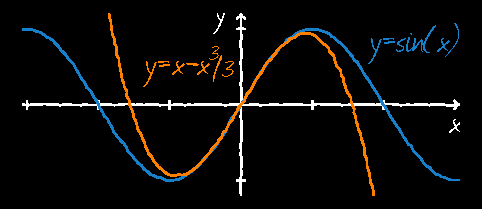
\includegraphics[width=.45\paperwidth]{figure/titlepage/dlsin}
    \end{center}
\end{textblock}

\begin{textblock}{.4}(.05,.65)
    \begin{center}
        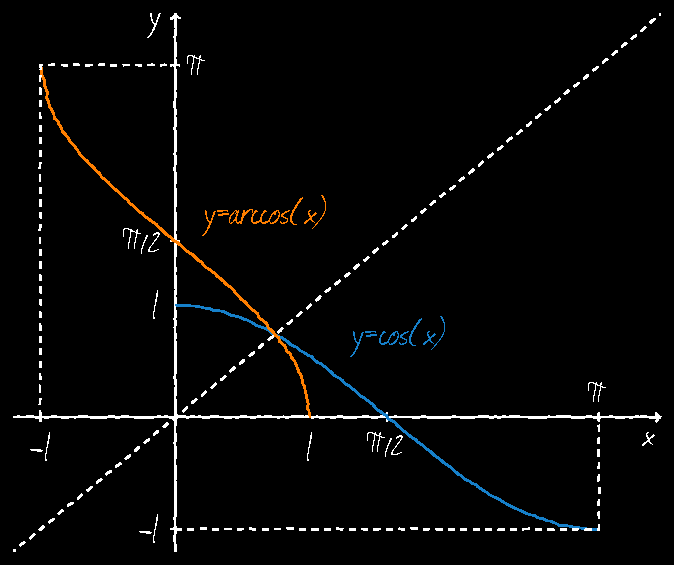
\includegraphics[width=.4\paperwidth]{figure/titlepage/arccos}
    \end{center}
\end{textblock}


\begin{textblock}{.6}(.05,.6)
    \noindent {\fontsize{20.74}{18}%
    \textcolor{white}{$u(z)=\frac{E_gZ_0}{(Z_g+Z_0)(1-\varGamma_g\varGamma_l \mathrm{e}^{-\mathrm{j}2\beta l})}\left( \mathrm{e}^{-\mathrm{j}\beta z} + \varGamma_l \mathrm{e}^{-\mathrm{j}2\beta l} \mathrm{e}^{\mathrm{j}\beta z}\right)$}}
\end{textblock}


\begin{textblock}{.4}(.4,.77)
    \noindent {\fontsize{17.28}{18}%
    \textcolor{white!80}{$\displaystyle 
    P_\mathrm{max}=\frac{E_\mathrm{max}^2ab\sqrt{\varepsilon_r}}{480\pi\xi}$}}
\end{textblock}

\begin{textblock}{.4}(.1,.93)
    \noindent {\fontsize{14.4}{18}%
    \textcolor{white!50}{$\displaystyle 
                \binom{n}{k} = \frac{n!}{k!(n-k)!}$}}
\end{textblock}


\begin{textblock}{.6}(.5,.69)
    \noindent {\fontsize{17.28}{18}%
    \textcolor{white!10}{$\displaystyle 
                \zeta_k = |a|^{1/n} \mathrm{e}^{i(\mathrm{arg}(a)+2k\pi)/n}$}}
\end{textblock}


\begin{textblock}{.3}(.75,.73)
    \noindent {\fontsize{17.28}{18}%
    \textcolor{white!10}{$\displaystyle \mathrm{e}^{i\pi}+1=0$}}
\end{textblock}



\null\newpage\pagestyle{nexus}

\tableofcontents

% !TeX root = Microwave.tex
\chapter{Transmission Line Theory 传输线理论 }
\setlength{\parindent}{2\ccwd}
\section{Transmission Line Equation 传输线方程 }

% \paragraph{Plane Waves in a Lossless Medium}
% ~\\[-15pt]


% In a lossless medium, $\varepsilon,\,\mu\in\mathfrak{R}$, and so $k$ is real.

\subsection{微波传输线}
    良导体的集肤效应:
    \begin{equation}
        \alpha=\sqrt{\frac{\omega\mu\sigma}{2}}=\frac{1}{\delta}
    \end{equation}

    where $\alpha$ is the \emph{attenuation constant} and $\delta$ is the \emph{skin depth}.

\subsection{传输线方程}
    微波传输线的四参数模型:
    \begin{subequations}
        \begin{numcases}{}
        -\frac{\partial u}{\partial z}=Ri+L \frac{\partial i}{\partial t}\\
        -\frac{\partial i}{\partial z}=Gu+C \frac{\partial u}{\partial t}
        \end{numcases}
    \end{subequations}
    对于时谐场:
    \begin{subequations}
        \begin{numcases}{}
        -\frac{\mathrm{d}u}{\mathrm{d}z}=i(R+\mathrm{j}\omega L)=Zi\\
        -\frac{\mathrm{d}i}{\mathrm{d}z}=u(G+\mathrm{j}\omega C)=Yu
        \end{numcases}
    \end{subequations}
    特别注意,这里的$R,\,Z$单位为\si{\ohm\per\metre},$G,\,Y$的单位为\si{\siemens\per\metre}。


\subsection{无耗传输线方程}
    无耗$\Rightarrow R=G=0$(导线上没有电阻或电纳)
    \begin{subequations}
        \begin{numcases}{}
        -\frac{\mathrm{d}u}{\mathrm{d}z}=\mathrm{j}\omega Li \label{Equ: Lossless Medium dudz}\\
        -\frac{\mathrm{d}i}{\mathrm{d}z}=\mathrm{j}\omega Cu \label{Equ: Lossless Medium didz}
        \end{numcases}
    \end{subequations}
    将式 (\ref{Equ: Lossless Medium dudz})代入式 (\ref{Equ: Lossless Medium didz})或者反之,可以解得:
    \begin{subequations}
        \begin{numcases}{}
        \frac{\mathrm{d}^2u}{\mathrm{d}z^2}+\beta^2u=0 \label{Equ: Lossless Transmission d2udz2}\\
        \frac{\mathrm{d}^2i}{\mathrm{d}z^2}+\beta^2i=0 \label{Equ: Lossless Transmission d2idz2}
        \end{numcases}
    \end{subequations}
    其中$\beta=\omega\sqrt{LC}$为相位常数。
    解此二阶微分方程,得:
    \begin{subequations}
        \begin{numcases}{}
        u(z)=A_1 \mathrm{e}^{-\mathrm{j}\beta z}+A_2 \mathrm{e}^{\mathrm{j}\beta z}\label{Equ: Lossless Transmission u(z)}\\
        i(z)=\frac{1}{Z_0}\left(A_1 \mathrm{e}^{-\mathrm{j}\beta z} {\color{red}\,-\,} A_2 \mathrm{e}^{\mathrm{j}\beta z}\right)\label{Equ: Lossless Transmission i(z)}
        \end{numcases}
    \end{subequations}
    其中,$Z_0=\sqrt{\frac{L}{C}}$为特性阻抗,单位为\si{\ohm}。确定$A_1,\,A_2$还需边界条件。

    \paragraph{本征模思想:}任何传输线上的电压是入射波和反射波的叠加,其形式确定如式(\ref{Equ: Eigenmode u=(u+)+(u-)}),不同传输线的区别仅在与入射波和反射波的成分不同。
    \begin{subequations}\label{Equ: Eigenmode u(z) and i(z)}
        \begin{numcases}{}
            u(z)=u^+_0 \mathrm{e}^{-\mathrm{j}\beta z}+u^-_0 \mathrm{e}^{\mathrm{j}\beta z}\label{Equ: Eigenmode u=(u+)+(u-)}\\
            i(z)=\frac{u^+_0}{Z_0} \mathrm{e}^{-\mathrm{j}\beta z} {\color{red}\,-\,} \frac{u^-_0}{Z_0} \mathrm{e}^{\mathrm{j}\beta z}
        \end{numcases}
    \end{subequations}

\subsection{无耗传输线的边界条件}\label{Sec: Boundary conditions of lossless transmission lines}
    以源端为原点建立$z$轴,正方向为负载方向。以终端为原点建立$z'$轴,正方向为电源方向。


    设导线长度为$l$,则导线上源端坐标系下坐标为$z=z_0$的点,在另一个坐标系下表示为$z'=l-z_0$。

    \begin{enumerate}
        \item {\bfseries 终端边界条件:}已知负载上的电压$U_l$、电流$I_l$
            \begin{equation}
                \begin{bmatrix}
                    u(z')\\
                    i(z')
                \end{bmatrix}
                =
                \begin{bmatrix}
                    \cos{\beta z'}&\mathrm{j}Z_0\sin{\beta z'}\\
                    \mathrm{j}\frac{1}{Z_0}\sin{\beta z'}&\cos{\beta z'}
                \end{bmatrix}
                \begin{bmatrix}
                    u(l)\\
                    i(l)
                \end{bmatrix}\label{Equ: u(z'), i(z')|u(l), i(l)}
            \end{equation}
            其中,$z'=l-z$。虽然这种用A参数矩阵描述的二端口网络形式很好记,但有时还会用到它的本征模形式:
            \begin{subequations}
                \begin{numcases}{}
                    u(z)=\frac{1}{2}(U_l+Z_0I_l)\mathrm{e}^{\mathrm{j}\beta l} \,\mathrm{e}^{-\mathrm{j}\beta z}+\frac{1}{2}(U_l-Z_0I_l)\mathrm{e}^{-\mathrm{j}\beta l}\, \mathrm{e}^{\mathrm{j}\beta z}\\
                    i(z)=\frac{1}{2Z_0}(U_l+Z_0I_l)\mathrm{e}^{\mathrm{j}\beta l}\, \mathrm{e}^{-\mathrm{j}\beta z} {\color{red}\,-\,} \frac{1}{2Z_0}(U_l-Z_0I_l)\mathrm{e}^{-\mathrm{j}\beta l}\, \mathrm{e}^{\mathrm{j}\beta z}
                \end{numcases}
            \end{subequations}
            或$z'$下
            \begin{subequations}\label{Equ: 无耗传输线终端边界条件电压电流表达式z'}
                \begin{numcases}{}
                    u(z')=\frac{1}{2}(U_l+Z_0I_l)\mathrm{e}^{\mathrm{j}\beta z'} +\frac{1}{2}(U_l-Z_0I_l)\mathrm{e}^{-\mathrm{j}\beta z'}\\
                    i(z')=\frac{1}{2Z_0}(U_l+Z_0I_l)\mathrm{e}^{\mathrm{j}\beta z'} {\color{red}\,-\,} \frac{1}{2Z_0}(U_l-Z_0I_l)\mathrm{e}^{-\mathrm{j}\beta z'}
                \end{numcases}
            \end{subequations}
        \item {\bfseries 源端边界条件:}已知源端处双导线之间电压$U_0$、电流$I_0$
            \begin{equation}
                \begin{bmatrix}
                    u(z)\\
                    i(z)
                \end{bmatrix}
                =
                \begin{bmatrix}
                    \cos{\beta z}&-\mathrm{j}Z_0\sin{\beta z}\\
                    -\mathrm{j}\frac{1}{Z_0}\sin{\beta z}&\cos{\beta z}
                \end{bmatrix}
                \begin{bmatrix}
                    u(0)\\
                    i(0)
                \end{bmatrix}\label{Equ: u(z), i(z)|u(0), i(0)}
            \end{equation}
            它的本征模形式为:
            \begin{subequations}
                \begin{numcases}{}
                    u(z)=\frac{1}{2}(U_0+Z_0I_0) \mathrm{e}^{-\mathrm{j}\beta z}+\frac{1}{2}(U_0-Z_0I_0) \mathrm{e}^{\mathrm{j}\beta z}\\
                    i(z)=\frac{1}{2Z_0}(U_0+Z_0I_0) \mathrm{e}^{-\mathrm{j}\beta z} {\color{red}\,-\,} \frac{1}{2Z_0}(U_0-Z_0I_0) \mathrm{e}^{\mathrm{j}\beta z}
                \end{numcases}
            \end{subequations}
        \item {\bfseries 电源、阻抗条件:}已知电源电压$E_g$、内阻$Z_g$,负载$Z_l$


            定义{\color{orange} 电源反射系数}和{\color{orange} 负载反射系数}:
            \begin{align}
                \varGamma_g&=\frac{Z_g-Z_0}{Z_g+Z_0}\\
                \varGamma_l&=\frac{Z_l-Z_0}{Z_l+Z_0}
            \end{align}
            $\varGamma_g$反映了电源阻抗与特征阻抗的匹配程度,即体现了电源吸收反射波能力的大小。
            $\varGamma_l$反应了负载与特征阻抗的匹配程度,不匹配的负载是反射波的源。


            {\color{red}NOTE:} 在稳态下只有$\varGamma_l$起作用,当$\varGamma_l=0$时,$\varGamma_g$没有意义。

            \begin{numcases}{}
                \mbox{源端:}u(0)=E_g-i(0)Z_g\xlongequal{i(0)=\frac{1}{Z_0}(A_1-A_2)}E_g-\frac{Z_g}{Z_0}(A_1-A_2)=A_1+A_2\notag\\
                \mbox{终端:}u(l)=i(l)Z_l\xlongequal{i(l)=\frac{1}{Z_0}(A_1 \mathrm{e}^{-\mathrm{j}\beta l}-A_2 \mathrm{e}^{\mathrm{j}\beta l})}Z_l\frac{1}{Z_0}(A_1 \mathrm{e}^{-\mathrm{j}\beta l}-A_2 \mathrm{e}^{\mathrm{j}\beta l})=A_1 \mathrm{e}^{-\mathrm{j}\beta l}+A_2 \mathrm{e}^{\mathrm{j}\beta l}\notag
            \end{numcases}

            由此得到关于$A_1,A_2$的方程组,使用\emph{Cramer's Rule}解出$A_1,A_2$,代入式(\ref{Equ: Lossless Transmission u(z)})和式(\ref{Equ: Lossless Transmission i(z)})得:
            \begin{subequations}
                \begin{numcases}{}
                    u(z)=\frac{E_gZ_0}{(Z_g+Z_0)(1-\varGamma_g\varGamma_l \mathrm{e}^{-\mathrm{j}2\beta l})}\left( \mathrm{e}^{-\mathrm{j}\beta z} + \varGamma_l \mathrm{e}^{-\mathrm{j}2\beta l} \mathrm{e}^{\mathrm{j}\beta z}\right)\label{Equ: u(z)|E_g, Z_h, Z_l}\\
                    i(z)=\frac{E_g}{(Z_g+Z_0)(1-\varGamma_g\varGamma_l \mathrm{e}^{-\mathrm{j}2\beta l})}\left( \mathrm{e}^{-\mathrm{j}\beta z} {\color{red}\,-\,} \varGamma_l \mathrm{e}^{-\mathrm{j}2\beta l} \mathrm{e}^{\mathrm{j}\beta z}\right)\label{Equ: i(z)|E_g, Z_h, Z_l}
                \end{numcases}
            \end{subequations}
        \end{enumerate}


\section{Transmission Analysis \Rmnum{1} 传输状态分析 \Rmnum{1} }

\begin{table}[ht]
    \setlength{\belowrulesep}{-5mm} %在线条[不包括\bottomrule]下面增加一段垂直距离
    \setlength{\aboverulesep}{-5mm} %在线条[不包括\toprule]上面增加一段垂直距离
    \centering
    \resizebox{\textwidth}{!}
    {
    \begin{tabular}{c}
        \toprule
        \hspace{15cm}~\\
        \hline
    \end{tabular}
    }
    \textbf{传输线的三个工作参数:反射系数、输入阻抗、驻波比}
    \resizebox{\textwidth}{!}
    {
    \begin{tabular}{c}
        \hline
        \hspace{15cm}~\\
        \bottomrule
    \end{tabular}
    }
\end{table}

\subsection{任意位置的反射系数}
    \subsubsection{反射系数$\varGamma(z)$}
    通常所说的反射系数,指的是从负载方向反射回电源方向的电压反射系数,常定义在$z'$坐标系下,记作$\varGamma(z')$
    \begin{equation}
        \varGamma(z')=\frac{u^-(z')}{u^+(z')}=\frac{u^-_l \mathrm{e}^{-\mathrm{j}\beta z'}}{u^+_l \mathrm{e}^{\mathrm{j}\beta z'}}=\varGamma_l \mathrm{e}^{-\mathrm{j}2\beta z'}\label{Equ: Reflection Coefficient at z'}
    \end{equation}
    \begin{center}
        $\varGamma(z'=l)$是否等于$\varGamma_g$? ——  {\color{red} 否。它们是完全独立的}
    \end{center}
    其中$u^+_l$即将$z=l$代入章节\ref{Sec: Boundary conditions of lossless transmission lines}中的本征模电压表达式,但只取向$z+$方向(也即$z'-$方向)传播的分量;同理,$u^-_l$即负载处向$z-$方向(也即$z'$方向)的电压分量。{\color{gray}可以利用第三种边界条件来验证一下, $u^+_l,\, u^-_l$分别为:
    \begin{subequations}
        \begin{numcases}{}
            u^+_l=u^+(z=l)=u^+(z'=0)=\frac{E_gZ_0 \mathrm{e}^{-\mathrm{j}\beta l}}{(Z_g+Z_0)(1-\varGamma_g\varGamma_l \mathrm{e}^{-\mathrm{j}2\beta l})}\\
            u^-_l=u^-(z=l)=u^-(z'=0)=\frac{E_gZ_0 \varGamma_l\mathrm{e}^{-\mathrm{j}\beta l}}{(Z_g+Z_0)(1-\varGamma_g\varGamma_l \mathrm{e}^{-\mathrm{j}2\beta l})}
        \end{numcases}
    \end{subequations}
    可见它们的确满足$u^-_l=\varGamma_l u^+_l$
    }
    \paragraph{电流反射系数:}
    \begin{equation}
        \varGamma_I(z')=\frac{i^-(z')}{i^+(z')}=\frac{i^-_l \mathrm{e}^{-\mathrm{j}\beta z'}}{i^+_l \mathrm{e}^{\mathrm{j}\beta z'}}{\color{red}\,=\frac{-u^-(z')/Z_0}{u^+(z')/Z_0}=-\varGamma(z')}\label{Equ: Reflection Coefficient of current at z'}
    \end{equation}
    \paragraph{使用前向电压电流和反射系数表示任意位置的电压电流:}(称$z+$方向为前向)
    ~\\[-15pt]

    根据\hyperref[Equ: Reflection Coefficient at z']{式(\ref*{Equ: Reflection Coefficient at z'})}和\hyperref[Equ: Reflection Coefficient of current at z']{式(\ref*{Equ: Reflection Coefficient of current at z'})},将入射波与反射波相加:
    \begin{subequations}\label{Equ: 电压或电流波的叠加}
        \begin{numcases}{}
            u(z')=u^+(z')\left[1+\varGamma(z')\right]=u^+_l(1+\varGamma_l \mathrm{e}^{-\mathrm{j}2\beta z'})\mathrm{e}^{\mathrm{j}\beta z'}\\
            i(z')=i^+(z')\left[1-\varGamma(z')\right]=i^+_l(1-\varGamma_l \mathrm{e}^{-\mathrm{j}2\beta z'})\mathrm{e}^{\mathrm{j}\beta z'}
        \end{numcases}
    \end{subequations}

    \paragraph{输入阻抗与特征阻抗通过反射系数转化:}
    ~\\[-15pt]

    上式所示的方程组上下相除可以得到任意位置输入阻抗$Z(z')$和传输线特征阻抗$Z_0$的关系:
    \begin{equation}
        Z(z')=Z_0\frac{1+\varGamma(z')}{1-\varGamma(z')}\label{Equ: Z(z')<-->Z_0}
    \end{equation}

    \begin{boxedminipage}{\textwidth}
        \vspace{5pt}
        注意各种阻抗的区别和关系:
        \begin{equation*}
        \mbox{}
        \begin{cases}
                \mbox{输入阻抗:}\mbox{(入射反射叠加)电压波与(入射反射叠加)电流波的比值} \\
                \mbox{特性阻抗:}\mbox{ 前向电压波与前向电流波的比值;或后向电压波与后向电流波的比值的相反数} \\
                \mbox{波阻抗:} \mbox{前向电场与前向磁场的比值}
        \end{cases}
        \end{equation*}
    \end{boxedminipage}


    \paragraph{反射系数的性质:}
    \begin{enumerate}
        \item 无耗传输系统中,\underline{反射系数的模值处处相等$|\varGamma(z')|=|\varGamma_l|$},辐角与移动的距离成正比;
        \item 反射系数呈周期性,关于电长度$\theta$的周期为$\pi$,关于$z'$的周期为$\frac{\lambda_g}{2}=\frac{\pi}{\beta}$。
        \item 反射系数模值不大于1(可从能量守恒的角度理解)。
    \end{enumerate}

\subsection{任意位置的输入阻抗}
    \subsubsection{输入阻抗$Z(z)$}
    输入阻抗是一个宏观参数,并不是只和入射波有关,而是导线在\underline{稳态下}的电压与流过此处的电流之比。在$z'$坐标系中,任一点的输入阻抗为:
    \begin{equation}
        Z(z')=\frac{u(z')}{i(z')}
            \xlongequal[\mbox{\scriptsize(终端边界条件)}]{\mbox{式(\ref{Equ: u(z'), i(z')|u(l), i(l)})}}
        \frac{U_l\cos{\beta z'}+\mathrm{j}Z_0I_l\sin{\beta z'}}{\mathrm{j}\frac{1}{Z_0}U_l\sin{\beta z'}+I_l\cos{\beta z'}}
            \xlongequal[\mbox{\scriptsize(同除$I_l\cos{\beta z'}$)}]{Z_l=\frac{U_l}{I_l}}
        \frac{\frac{Z_l}{Z_0}+\mathrm{j}\tan{\beta z'}}{\mathrm{j}\frac{Z_l}{Z_0}\tan{\beta z'}+1}
    \end{equation}
    该式也可以由\hyperref[Equ: Z(z')<-->Z_0]{式(\ref*{Equ: Z(z')<-->Z_0})} 代入$\varGamma_l$得到:
    \begin{align}
        Z(z')&=Z_0\frac{1+\varGamma_l \mathrm{e}^{-\mathrm{j}2\beta z'}}{1- \varGamma_l \mathrm{e}^{-\mathrm{j}2\beta z'}}
        % \xlongequal[\mbox{同乘$(Z_l+Z_0)$}]{\mbox{同乘$\mathrm{e}^{\mathrm{j}\beta z'}$}}
        \quad\mbox{(上下同乘$(Z_l+Z_0)\mathrm{e}^{\mathrm{j}\beta z'}$)}\notag\\
        &=Z_0\frac{(Z_l+Z_0)(\cos\beta z'+\mathrm{j}\sin\beta z')+(Z_l-Z_0)(\cos\beta z'-\mathrm{j}\sin\beta z')}
            {(Z_l+Z_0)(\cos\beta z'+\mathrm{j}\sin\beta z')-(Z_l-Z_0)(\cos\beta z'-\mathrm{j}\sin\beta z')}\notag\\
        &=Z_0\frac{2Z_l\cos\beta z'+2Z_0 \mathrm{j}\sin\beta z'}{2Z_l \mathrm{j}\sin\beta z'+2Z_0 \cos\beta z'}
            \quad\mbox{(上下同除以$2\cos\beta z'$)}\notag\\
        &=Z_0\frac{Z_l+Z_0 \mathrm{j}\tan\beta z'}{Z_l \mathrm{j}\tan\beta z'+Z_0}\label{Equ: 使用终端反射系数表示输入阻抗}
    \end{align}

    \paragraph{输入阻抗的性质:}

    \begin{enumerate}
        \item 通过控制传输长度,微波传输线对输入阻抗具有阻抗变换作用;


        常利用电长度$\theta=\beta z$取值为$m\pi+\frac{\pi}{2}$(即距离$(\frac{1}{2}m+\frac{1}{4})\lambda_g$)来实现阻抗的反演变换:
        \begin{align*}
            Z(z'\pm\frac{1}{4}\lambda_g)
            &=Z_0\frac{1+\varGamma_l \mathrm{e}^{(-\mathrm{j}2\beta z'\mp\mathrm{j}\pi)}}{1- \varGamma_l \mathrm{e}^{(-\mathrm{j}2\beta z'\mp\mathrm{j}\pi)}}\\
            &=Z_0\frac{1-\varGamma_l \mathrm{e}^{-\mathrm{j}2\beta z'}}{1+\varGamma_l \mathrm{e}^{-\mathrm{j}2\beta z'}}\\
            &=Z_0^2 \frac{1}{Z_0\frac{1+\varGamma_l \mathrm{e}^{-\mathrm{j}2\beta z'}}{1-\varGamma_l \mathrm{e}^{-\mathrm{j}2\beta z'}}}\\
            &=\frac{Z_0^2}{Z(z')}\doteq Z_0^2Y(z')
        \end{align*}
        \item 输入阻抗呈周期性,与反射系数的周期相同。

    \end{enumerate}

    \paragraph{总结:}任意位置的反射系数和输入阻抗及其转换关系
    \begin{figure}[htp]
        \centering
        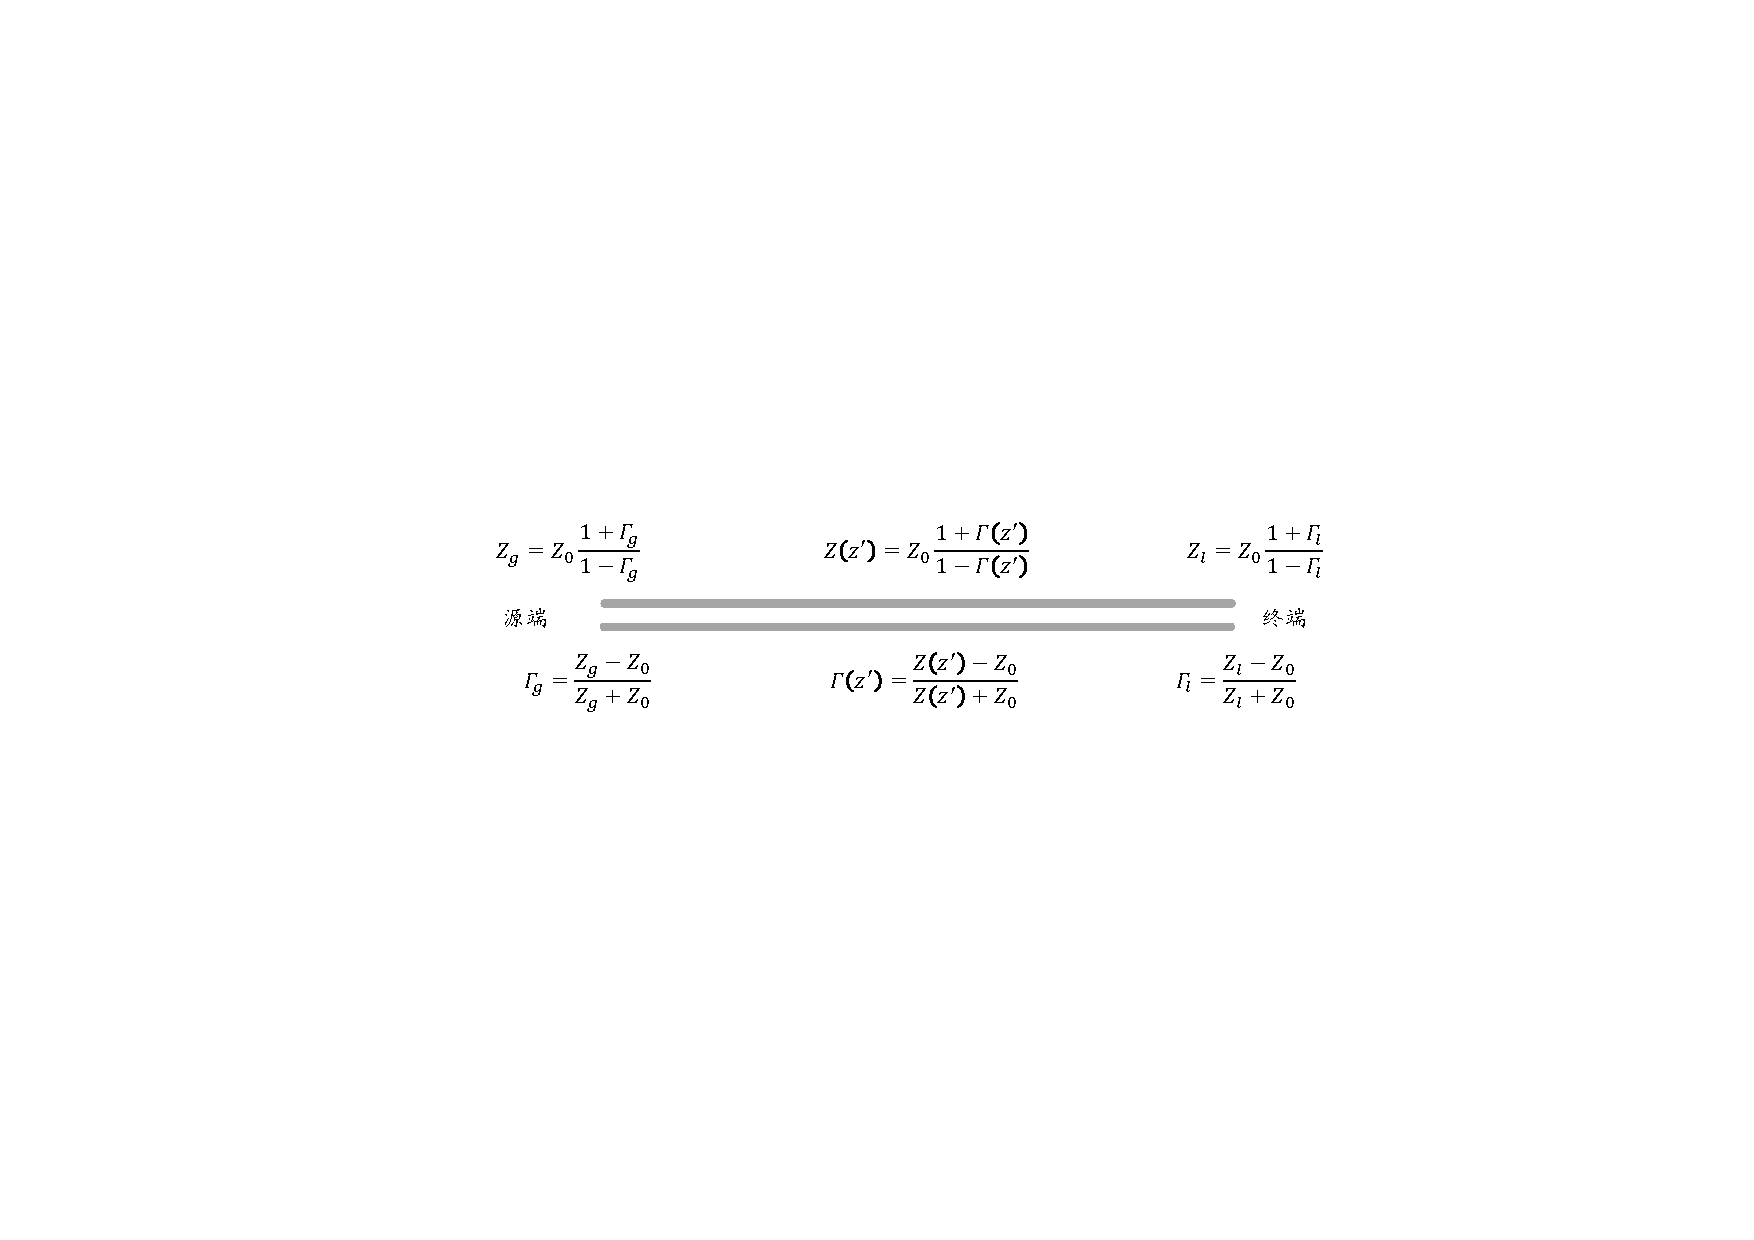
\includegraphics[width=14cm]{figure/1-1.pdf}
    \end{figure}

\subsection{电压驻波比——传输系统的不变量}
    电压驻波比(Voltage Standing Wave Ratio)\emph{abbr.} VSWR,也称驻波比(\emph{abbr.} SWR),定义为:
    \begin{equation}
        \rho=\frac{1+\left\vert\varGamma_l\right\vert}{1-\left\vert\varGamma_l\right\vert}\in[1,\infty)
    \end{equation}
    对于一个确定的传输系统,由于负载确定,所以$\varGamma_l$的模值确定,因此$\rho$是定值。


    根据 \hyperref[Equ: 电压或电流波的叠加]{式(\ref*{Equ: 电压或电流波的叠加})} ,电压或电流的叠加波振幅的极值只会在$\mathrm{e}^{\mathrm{j}\beta z'}=\pm 1$时取到。若已知电压波或电流波振幅极值,则驻波比可计算如下:
    \begin{align}
        \rho
        &=\frac{u^+(z')(1+|\varGamma_l|)}{u^+(z')(1-|\varGamma_l|)}
        =\frac{|u(z')|_\mathrm{max}}{|u(z')|_\mathrm{min}}\\
        &=\frac{i^+(z')(1+|\varGamma_l|)}{i^+(z')(1-|\varGamma_l|)}
        =\frac{|i(z')|_\mathrm{max}}{|i(z')|_\mathrm{min}}
    \end{align}

    在工程应用中,它可以衡量射频功率从功率源通过传输线传输到负载的效率。两个系统组件之间的最大功率传输发生在它们各自的阻抗匹配时。因此$\rho$越接近$1$,则驻波成分越少,效率越高。

    \paragraph{反射系数与驻波比的关系}
    \begin{equation*}
        \begin{array}{cccc}
            ~&\rho=\frac{1+\left\vert\varGamma_l\right\vert}{1-\left\vert\varGamma_l\right\vert}
            &\Leftrightarrow
            &|\varGamma_l|=|\varGamma(z')|=\dfrac{\rho-1}{\rho+1}\\
            \mbox{类比}&~&~&~\\
            ~&\frac{Z(z')}{Z_0}=\frac{1+\varGamma(z')}{1-\varGamma(z')}
            &\Leftrightarrow
            &\varGamma(z')=\dfrac{\frac{Z(z')}{Z_0}-1}{\frac{Z(z')}{Z_0}+1}
        \end{array}
    \end{equation*}

    \paragraph{输入阻抗与驻波比的关系}
    由于用反射系数可表示输入阻抗(\hyperref[Equ: Z(z')<-->Z_0]{式(\ref*{Equ: Z(z')<-->Z_0})}),而驻波比又可表示反射系数:
    \begin{equation}
        \varGamma(z')=|\varGamma_l|\mathrm{e}^{\mathrm{j}\varphi_l}\cdot\mathrm{e}^{-\mathrm{j}2\beta z'}=\frac{\rho-1}{\rho+1}\mathrm{e}^{\mathrm{j}(\varphi_l-2\beta z')}
    \end{equation}
    因此有
    \begin{align*}
        Z(z')
        &=Z_0\frac{1+\frac{\rho-1}{\rho+1}\mathrm{e}^{\mathrm{j}(\varphi_l-2\beta z')}}{1-\frac{\rho-1}{\rho+1}\mathrm{e}^{\mathrm{j}(\varphi_l-2\beta z')}}
        \quad\mbox{(上下同乘$(\rho+1)\mathrm{e}^{\mathrm{j}(-\frac{\varphi_l}{2}+\beta z')}$)}\\
        &=Z_0\frac{(\rho+1)\left[\cos(-\frac{\varphi_l}{2}+\beta z')+\mathrm{j}\sin(-\frac{\varphi_l}{2}+\beta z')\right]
                    +
                (\rho-1)\left[\cos(-\frac{\varphi_l}{2}+\beta z')-\mathrm{j}\sin(-\frac{\varphi_l}{2}+\beta z')\right]}
            {(\rho+1)\left[\cos(-\frac{\varphi_l}{2}+\beta z')+\mathrm{j}\sin(-\frac{\varphi_l}{2}+\beta z')\right]
                    -
                (\rho-1)\left[\cos(-\frac{\varphi_l}{2}+\beta z')-\mathrm{j}\sin(-\frac{\varphi_l}{2}+\beta z')\right]}\\
        &=Z_0\frac{2\rho\cos(-\frac{\varphi_l}{2}+\beta z')+2 \mathrm{j}\sin(-\frac{\varphi_l}{2}+\beta z')}
            {2\rho \mathrm{j}\sin(-\frac{\varphi_l}{2}+\beta z')+2 \cos(-\frac{\varphi_l}{2}+\beta z')}
        \quad\mbox{(上下同除以$2\cos(-\frac{\varphi_l}{2}+\beta z')$)}\\
        &=Z_0\frac{\rho+ \mathrm{j}\tan(-\frac{\varphi_l}{2}+\beta z')}
            {\rho \mathrm{j}\tan(-\frac{\varphi_l}{2}+\beta z')+1}
    \end{align*}
    该推导过程与\hyperref[Equ: 使用终端反射系数表示输入阻抗]{式(\ref*{Equ: 使用终端反射系数表示输入阻抗})}的推导有完全一致的思路。
    若再令$\Delta z=-\frac{1}{2\beta}(\varphi_l-\pi)$,则
    \begin{align}
        \mbox{上式}&=Z_0\frac{\rho+ \mathrm{j}\tan\beta(z'+\Delta z-\frac{\pi}{2\beta})}
            {\rho \mathrm{j}\tan\beta(z'+\Delta z-\frac{\pi}{2\beta})+1}\notag\\
        &=Z_0\frac{\rho-\mathrm{j}\frac{1}{\tan\beta(z'+\Delta z)}}
            {-\rho \mathrm{j}\frac{1}{\tan\beta(z'+\Delta z)}+1}\notag\\
        &=Z_0\frac{\rho\tan\beta(z'+\Delta z)-\mathrm{j}}
            {-\rho \mathrm{j}+\tan\beta(z'+\Delta z)}\notag\\
        &\;{\color{red}=Z_0\frac{\mathrm{j}\rho\tan\beta(z'+\Delta z)+1}
            {\rho+\mathrm{j}\tan\beta(z'+\Delta z)}}
    \end{align}
    实际上,由于$\varGamma_l=\frac{(R_l+\mathrm{j}X_l)-Z_0}{(R_l+\mathrm{j}X_l)+Z_0}=|\varGamma_l|\mathrm{e}^{\mathrm{j}\varphi_l}$,有以下二者等价:
    \begin{equation*}
        \Delta z=\frac{\lambda_g}{4\pi}\left[\arctan\frac{X_l}{Z_0+R_l}+\arctan\frac{X_l}{Z_0-R_l}\right] \Leftrightarrow \Delta z=-\frac{1}{2\beta}(\varphi_l-\pi)
    \end{equation*}

    坐标平移$z''=z'+\Delta z$ {\bfseries 使得 $z'+\Delta z=0$处始终为电压波节点}。
    因此有以下推论:
    \begin{enumerate}
        \renewcommand*\labelenumi{(\theenumi)}
        \item 电压波节点处,$z'+\Delta z=\frac{m}{2}\lambda_g$,此时输入阻抗
            \begin{equation}
                R_\mathrm{min}=Z_0\frac{\mathrm{j}\rho\cdot0+1}
                                        {\rho+\mathrm{j}\cdot0}
                =\frac{Z_0}{\rho}
                =\frac{|u(z')|_\mathrm{min}}
                        {|i(z')|_\mathrm{max}}
            \end{equation}
            为纯电阻,这是因为此处传输线处于LC串联谐振状态。
        \item 电压波腹点处,$z'+\Delta z=(\frac{m}{2}+\frac{1}{4})\lambda_g$,此时输入阻抗
            \begin{equation}
                R_\mathrm{max}=Z_0\frac{\mathrm{j}\rho\cdot\infty+1}
                                        {\rho+\mathrm{j}\cdot\infty}
                =\rho Z_0
                =\frac{|u(z')|_\mathrm{max}}
                        {|i(z')|_\mathrm{min}}
            \end{equation}
            为纯电阻,这是因为此处传输线处于LC并联谐振状态。
    \end{enumerate}

    \paragraph{功率与驻波比}
    特殊地,在波节点和波腹点处,由于电压电流波同相,因此:
    \begin{subequations}
        \begin{numcases}{\mbox{}}
            P(z'=-\Delta z+\frac{m}{2}\lambda_g)=\frac{1}{2}|u(z')|_\mathrm{min}|i(z')|_\mathrm{max}=\frac{1}{2}\frac{|i|^2_\mathrm{max}Z_0}{\rho} \\
            P(z'=-\Delta z+[\frac{m}{2}+\frac{1}{4}]\lambda_g)=\frac{1}{2}|u(z')|_\mathrm{max}|i(z')|_\mathrm{min}=\frac{1}{2}\frac{|u|^2_\mathrm{max}}{\rho Z_0}
        \end{numcases}
    \end{subequations}

\subsection{行驻波功率关系}

    一般地,任意点处的传输功率:
    \begin{align}
        P(z')&=\frac{1}{2}\Re\left[u(z')i^*(z')\right]\\
        &=\frac{1}{2}\Re\left[u^+_l \mathrm{e}^{\mathrm{j}\beta z'}(1+\varGamma(z'))\cdot\frac{u^{+*}_l}{Z_0}\mathrm{e}^{-\mathrm{j}\beta z'}(1-\varGamma^*(z'))\right]\\
        &=\frac{1}{2}\Re\left\{\frac{U^{+^2}_{lm}}{Z_0}\left[1+\varGamma(z')-\varGamma^*(z')-|\varGamma(z')|^2\right]\right\}\\
        &=\frac{1}{2}\frac{U^{+^2}_{lm}}{Z_0}-\frac{1}{2}\frac{U^{+^2}_{lm}}{Z_0}|\varGamma(z')|^2
    \end{align}
    其中,入射功率:
    \begin{equation}
        P_i(z')=\frac{1}{2}\frac{U^{+^2}_{lm}}{Z_0}
    \end{equation}
    反射功率:
    \begin{equation}
        P_r(z')=\frac{1}{2}\frac{U^{+^2}_{lm}}{Z_0}|\varGamma(z')|^2
    \end{equation}


    \begin{table}[ht]
        \setlength{\belowrulesep}{-5mm} %在线条[不包括\bottomrule]下面增加一段垂直距离
        \setlength{\aboverulesep}{-5mm} %在线条[不包括\toprule]上面增加一段垂直距离
        \centering
        \resizebox{\textwidth}{!}
        {
        \begin{tabular}{c}
            \toprule
            \hspace{15cm}~\\
            \hline
        \end{tabular}
        }
        \textbf{传输线的三种工作状态:行波、全驻波、行驻波}
        \resizebox{\textwidth}{!}
        {
        \begin{tabular}{c}
            \hline
            \hspace{15cm}~\\
            \bottomrule
        \end{tabular}
        }
    \end{table}

\subsection{传输线的行波状态}
    当负载是匹配的($Z_l=Z_0$)或者传输线无限长时,传输线处于行波状态。此时:
    \begin{itemize}
        \item $\varGamma(z')=0$ (反射系数为0,没有反射波)
    \item $u(z)=u^+_0 \mathrm{e}^{-\mathrm{j}\beta z}$,$u$和$i$都只有$z+$向传播的分量。因此输入阻抗等于特征阻抗:$Z(z')=Z_0$(也可以由式(\ref{Equ: Z(z')<-->Z_0})代入$\varGamma(z')=0$得出)
        \item 此时传输线上的电压电流的瞬时表达式:
    \end{itemize}
    \begin{subequations}
        \begin{numcases}{}
            u(z,t)=U^+_{0}(t) \mathrm{e}^{-\mathrm{j}\beta z}=U_{0\mathrm{m}}\cos(\omega t -\beta z + \varphi_0) \\
            i(z,t)=\frac{U^+_{0}(t)}{Z_0} \mathrm{e}^{-\mathrm{j}\beta z}=I_{0\mathrm{m}}\cos(\omega t -\beta z + \varphi_0)
        \end{numcases}
    \end{subequations}

\subsection{传输线的全驻波状态}
    定义$|\varGamma(z')|=1$时传输线处于全驻波状态。\underline{可证明${\color{red}|\varGamma_l|}=1$的充要条件是$Z_l=\mathrm{j}X_l\in\Im$}。


    我们考虑$Z_l$为纯虚数的两种极端情况:$Z_l=\mathrm{j}0$(短路状态)和$Z_l=\mathrm{j}\infty$(开路状态),再导出一般情况。
    \begin{enumerate}
        \item {\bfseries 短路状态}(\underline{标准状态}):代入$Z_l=\mathrm{j} 0$
        \begin{itemize}
            \item $\varGamma_l=\frac{0-Z_0}{0+Z_0}=-1$
            \item 任一点反射系数:
            $\varGamma(z')\doteq\varGamma_l\mathrm{e}^{-\mathrm{j}2\beta z'}=\mathrm{e}^{\mathrm{j}(\pi-2\beta z')}$
            \item $u^-_l=\varGamma_l u^+_l=-u^+_l$,终端处反射波电压为入射波电压的相反数,叠加始终为0,因此一定在终端形成电压波节点;$i^-_l=-\varGamma_l i^+_l=i^+_l$,终端处反射波电流等于入射波电流,叠加始终最大,因此一定在终端形成电流波腹点;
            \item 此时传输线上的电压电流的表达式:
            \begin{subequations}\label{Equ: 全驻波电压电流表达式}
                \begin{numcases}{}
                    u(z',t)=U^+_{l}(t) \mathrm{e}^{\mathrm{j}\beta z'}+\left[\varGamma_l U^+_{l}(t)\right] \mathrm{e}^{-\mathrm{j}\beta z'}=2\mathrm{j}U^+_{l}(t)\sin(\beta z') \\
                    i(z',t)=I^+_{l}(t) \mathrm{e}^{\mathrm{j}\beta z'}+\left[-\varGamma_l I^+_{l}(t)\right] \mathrm{e}^{-\mathrm{j}\beta z'}=2I^+_{l}(t)\cos(\beta z')
                \end{numcases}
            \end{subequations}

                注意,在推导瞬时表达式时:类比
                \begin{subequations}
                    \begin{numcases}{}
                        u^+(z,t)={\color{red}U_{0\mathrm{m}}\cos(\omega t-\beta z + \varphi_0)}=U_{l\mathrm{m}}\cos\left[\omega t-\beta (z-l) + \varphi_0\right]\\
                        u^+(z',t)=U_{0\mathrm{m}}\cos\left[\omega t-\beta (l-z') + \varphi_0\right]={\color{red}U_{l\mathrm{m}}\cos\left(\omega t+\beta z' + \varphi_0\right)}
                    \end{numcases}
                \end{subequations}
                得到:
                % \parbox{\textwidth}{
                \begin{subequations}
                    \begin{numcases}{}
                        U^+_{0}(t)\doteq u^+(z=0,t)=u^+(z'=l,t)\notag\\
                        \qquad={\color{red}U_{0\mathrm{m}}\cos(\omega t +\varphi_0)}=U_{l\mathrm{m}}\cos(\omega t +\beta l+\varphi_0)\\
                        U^+_{l}(t)\doteq u^+(z=l,t)=u^+(z'=0,t)\notag\\
                        \qquad=U_{0\mathrm{m}}\cos(\omega t -\beta l+\varphi_0)={\color{red}U_{l\mathrm{m}}\cos(\omega t +\varphi_0)}
                    \end{numcases}
                \end{subequations}
                % }
                这里使用的符号$U^+_{l}(t)$是时域表达式,等于该点振幅幅值$U_{l \mathrm{m}}$与一时谐量;而使用小写字母的符号,形如$u^+_l$,通常是某一点的振幅$U^+_{l}(t)$乘以自然复指数$\mathrm{e}^{-\mathrm{j}k z}$的复数形式(例如\hyperref[Equ: 无耗传输线终端边界条件电压电流表达式z']{式(\ref*{Equ: 无耗传输线终端边界条件电压电流表达式z'})}、\hyperref[Equ: 全驻波电压电流表达式]{式(\ref*{Equ: 全驻波电压电流表达式})})。

                因此,
            \item 任一点输入阻抗:
            \begin{equation}
                Z(z')=\mathrm{j}Z_0\tan{\beta z'}{\color{gray}\,=Z_0\frac{0+\mathrm{j}Z_0\tan{\beta z'}}{Z_0+0}}
            \end{equation}
        \end{itemize}
        \item {\bfseries 开路状态} :代入$Z_l=\mathrm{j}\infty$
        \begin{itemize}
            \item $\varGamma_l=\frac{\mathrm{j}\infty-Z_0}{\mathrm{j}\infty+Z_0}\rightarrow 1$
            \item 任一点反射系数:
            $\varGamma(z')\doteq\varGamma_l\mathrm{e}^{-\mathrm{j}2\beta z'}=\mathrm{e}^{\mathrm{j}(0-2\beta z')}$
                \item $u^-_l=\varGamma_l u^+_l=u^+_l$,在终端形成电压波腹点;$i^-_l=-\varGamma_l i^+_l=-i^+_l$,在终端形成电流波节点;
            \item 此时传输线上的电压电流的表达式:
            \begin{subequations}
                \begin{numcases}{}
                    u(z',t)=U^+_{l}(t) \mathrm{e}^{\mathrm{j}\beta z'}+\left[\varGamma_l U^+_{l}(t)\right] \mathrm{e}^{-\mathrm{j}\beta z'}=2U^+_{l}(t)\cos(\beta z') \\
                    i(z',t)=I^+_{l}(t) \mathrm{e}^{\mathrm{j}\beta z'}+\left[-\varGamma_l I^+_{l}(t)\right] \mathrm{e}^{-\mathrm{j}\beta z'}=2\mathrm{j}I^+_{l}(t)\sin(\beta z')
                \end{numcases}
            \end{subequations}
            \item 任一点输入阻抗:
            \begin{equation}
                Z(z')=-\mathrm{j}Z_0\tan{\beta z'}{\color{gray}\,\leftarrow Z_0\frac{\mathrm{j}\infty+\mathrm{j}Z_0\tan{\beta z'}}{Z_0+\mathrm{j}\infty\tan{\beta z'}}}
            \end{equation}
        \end{itemize}

        \item {\bfseries 任意电抗负载} :代入$Z_l=\mathrm{j} X_l$
        \begin{itemize}
            \item $\varGamma_l=\frac{\mathrm{j}X_l-Z_0}{\mathrm{j}X_l+Z_0}=\mathrm{e}^{\mathrm{j}\varphi_l}$,则可以求出$\varphi_l=\pi-2\arctan\frac{X_l}{Z_0}$。
            % 且易知:$\varphi_l=\pi-$
            \item 任一点反射系数:
                \begin{equation}
                    \varGamma(z')\doteq\varGamma_l \mathrm{e}^{-2\mathrm{j}\beta z'}=\mathrm{e}^{\mathrm{j}(\varphi_l-2\beta z')}=\frac{Z(z')-Z_0}{Z(z')+Z_0}
                \end{equation}
            \item 任一点输入阻抗:
                \begin{align}
                    Z(z')&=\mathrm{j}Z_0\frac{\frac{X_l}{Z_0}+\tan{\beta z'}}{1-\frac{X_l}{Z_0}\tan{\beta z'}}\notag\\
                    &=\mathrm{j}Z_0\tan{\beta(z'+\Delta z)}\quad\mbox{(let $\tan{\beta \Delta z}=\frac{X_l}{Z_0}$)}
                \end{align}
                则可认为在新坐标系$z''=z'+\Delta z$下,任意电抗负载下与短路状态下的输入阻抗具有相同的形式。其中

                \begin{equation}
                    \Delta z=\frac{1}{\beta}\arctan\frac{X_l}{Z_0}=-\frac{1}{2\beta}(\varphi_l-\pi)
                \end{equation}


                特殊地,对于负载开路的情况,$\Delta z=\frac{\lambda_g}{4}\;(\beta \Delta z=90\si{\degree})$。


                若$\Delta z\geqslant0$,意味着原坐标轴$z'$向它的负方向平移$|\Delta z|$可以得到$z''$,反之需要向$z'+$方向平移。
            \item 传输线上电压电流表达式:
                \begin{subequations}
                        \begin{equation*}
                            \left\{
                        \begin{aligned}
                            u(z')&=u^+_l\left(\mathrm{e}^{\mathrm{j}\beta z'}+\varGamma_l\mathrm{e}^{-\mathrm{j}(\beta z')} \right)=u^+_l\left(\mathrm{e}^{\mathrm{j}\beta z'}+\mathrm{e}^{\mathrm{j}(\varphi_l-\beta z')} \right)\\
                            &=u^+_l \mathrm{e}^{\mathrm{j}\frac{1}{2}(\varphi_l-\pi)}\left(\mathrm{e}^{\mathrm{j}\left[\beta z'-\frac{1}{2}(\varphi_l-\pi)\right]}+\mathrm{e}^{\mathrm{j}\left[\frac{1}{2}(\varphi_l{\color{red}+}\pi)-\beta z'\right]} \right)\\
                            &=u^+_l \mathrm{e}^{\mathrm{j}\frac{1}{2}(\varphi_l-\pi)}\left(\mathrm{e}^{\mathrm{j}\left[\beta z'-\frac{1}{2}(\varphi_l-\pi)\right]}-\mathrm{e}^{\mathrm{j}\left[\frac{1}{2}(\varphi_l-\pi)-\beta z'\right]} \right)\\
                            &=u^+_l \mathrm{e}^{\mathrm{j}\frac{1}{2}(\varphi_l-\pi)}2 \mathrm{j}\sin{\left[\beta z'-\frac{1}{2}(\varphi_l-\pi) \right]}\\
                            &=2 \mathrm{j}u^+_l \mathrm{e}^{\mathrm{j}\frac{1}{2}(\varphi_l-\pi)}\sin{\left[\beta \left(z'+\fbox{$-\frac{1}{2\beta}(\varphi_l-\pi)$}\right) \right]}\\
                            i(z')&=2i^+_l\mathrm{e}^{\mathrm{j}\frac{1}{2}(\varphi_l-\pi)}\cos{\left[\beta \left(z'+\fbox{$-\frac{1}{2\beta}(\varphi_l-\pi)$}\right) \right]}
                    \end{aligned}\right.
                    \end{equation*}
                \end{subequations}
                方框内的部分即$\Delta z$。
                \paragraph{总结——全驻波任意电抗负载下各参数求法:}
                \begin{subequations}
                    \begin{numcases}{}
                        \varphi_l=\pi-2\arctan\frac{X_l}{Z_0}\\
                        \Delta z=-\frac{1}{2\beta}(\varphi_l-\pi)=\frac{\lambda_g}{2\pi}\arctan\frac{X_l}{Z_0}\\
                        \varGamma_l=\frac{\mathrm{j}X_l-Z_0}{\mathrm{j}X_l+Z_0}
                        % =-\frac{1-\mathrm{j}\frac{X_l}{Z_0}}{1+\mathrm{j}\frac{X_l}{Z_0}}
                        =\frac{\mathrm{j}\tan{\beta \Delta z}-1}{\mathrm{j}\tan{\beta \Delta z}+1} \\
                        Z(z')=\mathrm{j}Z_0\tan{\beta(z'+\Delta z)}
                    \end{numcases}
                \end{subequations}
        \end{itemize}
    \end{enumerate}


\section{Transmission Analysis \Rmnum{2} 传输状态分析 \Rmnum{2} }
\subsection{传输线的行驻波状态}
    行驻波状态是一般性的、有部分或全部反射的情况。
    \begin{subequations}
        \begin{numcases}{\mbox{一般地,任意确定负载的传输线:}}
            \varGamma_l=|\varGamma_l|\mathrm{e}^{\mathrm{j}\varphi_l} \,,\;\mbox{where}|\varGamma_l|\leqslant 1\\
            Z_l=R_l+\mathrm{j}X_l
        \end{numcases}
    \end{subequations}
    但在介绍时,仍从一种特殊情况出发:$Z_l=R_l<Z_0$,称为行驻波传输线的的标准状态。
    \begin{equation*}
    \mbox{传输线的一般情形:行驻波状态}
    \begin{cases}
        \mbox{标准状态:负载为小电阻}\\
        \mbox{任意状态:负载为任意阻抗}
    \end{cases}
    \end{equation*}
    \begin{enumerate}
        \item {\bfseries 小电阻负载}(\underline{标准状态})
        \begin{itemize}
            \item

            \item 任一点输入阻抗:
            \begin{equation}
                Z(z')=
            \end{equation}
        \end{itemize}
        \item {\bfseries 大电阻负载}
        \begin{itemize}
            \item

            \item 任一点输入阻抗:
            \begin{equation}
                Z(z')=
            \end{equation}
        \end{itemize}
        \item {\bfseries 任意阻抗负载} % $|\varGamma(z')|\leqslant 1$,此时:
        \begin{itemize}
            \item
            \item 此时传输线上的电压电流的表达式:
            \begin{subequations}
                \begin{numcases}{}
                    u(z',t)=\\
                    i(z',t)=
                \end{numcases}
            \end{subequations}
            \item 任一点输入阻抗:
            \begin{equation}
                Z(z')=
            \end{equation}
        \end{itemize}
    \end{enumerate}
    \paragraph{总结——行驻波任意阻抗负载下各参数求法:}
                \begin{subequations}
                    \begin{numcases}{}
                        \varphi_l=
                            \left\{\begin{aligned}
                                \pi-\left[\arctan\frac{X_l}{Z_0+R_l}+\arctan\frac{X_l}{Z_0-R_l}\right]\;,\quad R_l-Z_0<0\mbox{(小电阻)}\\
                                \arctan\frac{X_l}{R_l-Z_0}-\arctan\frac{X_l}{R_l+Z_0}\;,\quad R_l-Z_0>0\mbox{(大电阻)}
                            \end{aligned}\right.\label{Equ: phi_l} \\
                        \Delta z=\frac{1}{2\beta}(\pi-\varphi_l)\\
                            % \left\{\begin{aligned}
                            %     \frac{1}{2\beta}(\pi-\varphi_l)
                            %     % =\frac{\lambda_g}{4\pi}\left[\arctan\frac{X_l}{Z_0+R_l}+\arctan\frac{X_l}{Z_0-R_l}\right]
                            %         \,,\;\varphi_l>0\\
                            %     \frac{1}{2\beta}(\pi+\varphi_l)
                            %     % =\frac{\lambda_g}{4\pi}\left[\pi+\arctan\frac{X_l}{R_l+Z_0}-\arctan\frac{X_l}{R_l-Z_0}\right]
                            %         \,,\;\varphi_l<0
                            % \end{aligned}\right.\\
                        % \varGamma_l=\frac{\mathrm{j}X_l-Z_0}{\mathrm{j}X_l+Z_0}=-\frac{1-\mathrm{j}\frac{X_l}{Z_0}}{1+\mathrm{j}\frac{X_l}{Z_0}}=-\frac{1-\mathrm{j}\tan{\beta \Delta z}}{1+\mathrm{j}\tan{\beta \Delta z}} \\
                        Z(z')=Z_0\frac{1+\mathrm{j}\rho\tan{\beta(z'+\Delta z)}}{\rho+\mathrm{j}\tan{\beta(z'+\Delta z)}}
                    \end{numcases}
                \end{subequations}

\subsection{行驻波阻抗图形}
    距离终端最近的一个电压波节点到终端的距离为
    \begin{equation}
        d_\mathrm{min}=
        \left\{\begin{aligned}
            &-\Delta z \;,\quad \Delta z\leqslant0\\
            &\frac{1}{2}\lambda_g-\Delta z\;,\quad \Delta z>0
        \end{aligned}\right.
    \end{equation}
    等价于
    \begin{equation*}
        d_\mathrm{min}=
        \left\{\begin{aligned}
            &\frac{\lambda_g}{4\pi}\left(\varphi_l-\pi\right) \;,\quad \varphi_l\geqslant \pi\\
            &\frac{\lambda_g}{4\pi}\left(\pi+\varphi_l\right) \;,\quad \varphi_l < \pi
        \end{aligned}\right.
    \end{equation*}
    在用\hyperref[Equ: phi_l]{式(\ref*{Equ: phi_l})}求$\varphi_l$时,其值位于$(-\pi,2 \pi)$内,可以借助下图分析负载到最近电压波节点的距离。

    \begin{figure}[htp]
        \centering
        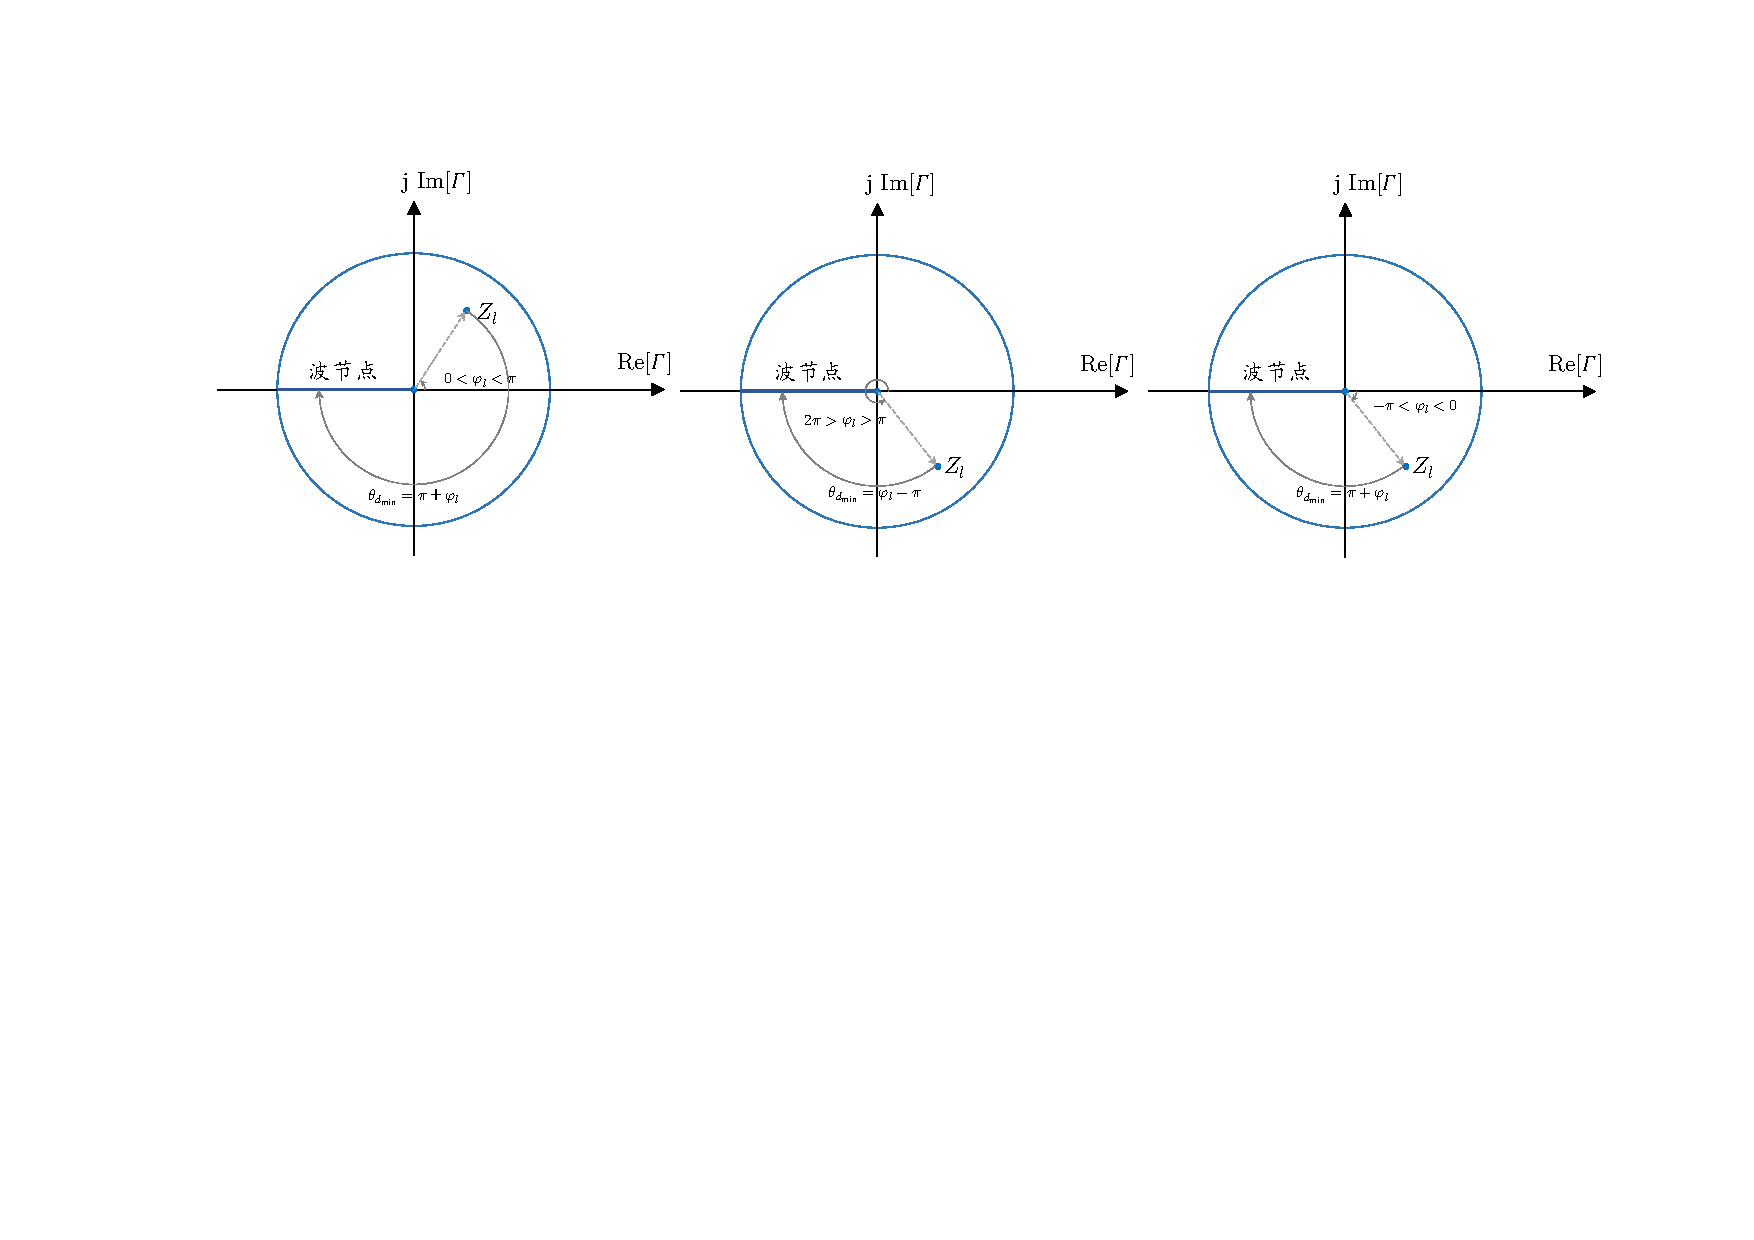
\includegraphics[width=15cm]{figure/1-2.pdf}
        \caption{\kaishu 负载到最近电压波节点的距离}\label{Fig: 负载到最近电压波节点的距离}
    \end{figure}

\section{Transmission Matrix Solution 传输矩阵解 }
\begin{center}
    \underline{约定:为了简便,本节使用的坐标系$z$为原点定义在终端,以  终端指向源端  为正方向的坐标系。}
\end{center}
因此无耗传输线模型式(\ref{Equ: Lossless Medium dudz}),(\ref{Equ: Lossless Medium didz})在当前坐标系下变为:
\begin{subequations}
    \begin{numcases}{}
        \frac{\mathrm{d}u}{\mathrm{d}z}=\mathrm{j}\omega Li \\
        \frac{\mathrm{d}i}{\mathrm{d}z}=\mathrm{j}\omega Cu
    \end{numcases}
\end{subequations}

\subsection{传输线段的矩阵解}
    \subsubsection{单边拉普拉斯变换求解无耗传输线模型}
    \begin{subequations}
        \begin{numcases}{}
            \mathscr{L}\left[\frac{\mathrm{d}u}{\mathrm{d}z}\right] \\
            d
        \end{numcases}
    \end{subequations}
    \subsubsection{传输线段矩阵}
    \subsubsection{传输线段矩阵导出输入阻抗和电压电流逆变换}
\subsection{传输矩阵的普遍理论}
    \subsubsection{传输线段的A参数矩阵}
\begin{equation}
    \begin{bmatrix}
        u_1\\i_1
    \end{bmatrix}
    =\begin{bmatrix}
        A_{11}&A_{12}\\
        A_{21}&A_{22}
    \end{bmatrix}
    \begin{bmatrix}
        u_2\\i_2
    \end{bmatrix}
\end{equation}

    \subsubsection{二端口网络性质的A参数描述}
        \begin{enumerate}
            \item 级联性质
            \begin{equation}
                \bm{A}=\prod_{i=1}^{N}\bm{A}_i
            \end{equation}
            \item 对称性质
            \begin{equation}
                A_{11}=A_{22}
            \end{equation}
            \item 无耗性质
            \begin{subequations}
                \begin{numcases}{\mbox{}}
                    A_{11},A_{22}\in\Re \\
                    A_{12},A_{21}\in\Im
                \end{numcases}
            \end{subequations}
            \item 互易性质
            \begin{equation}
                |\bm{A}|=1
            \end{equation}
            \item 阻抗变换性质
            \begin{equation}
                \begin{aligned}
                    Z_{in}&=\frac{u_1}{i_1}\\
                    &=\frac{A_{11}u_2+A_{12}i_2}{A_{21}u_2+A_{22}i_2}\\
                    &=\frac{A_{11}Z_l+A_{12}}{A_{21}Z_l+A_{22}}
                \end{aligned}
            \end{equation}
        \end{enumerate}
    
    \subsubsection{阻抗归一化的A参数矩阵}
    % 由于一个网络的端口电压和电流的关系由此处的特性阻抗所体现,因此A参数也必然和特性阻抗有关。
    此处的归一化,并非线性代数中的矩阵归一化,而是对电压波除和电流波做阻抗归一化,使其量纲变为\si{\V\per\sqrt{\ohm}}和\si{\A\sqrt{\ohm}},然后用这种归一化阻抗的电压波和电流波定义的A参数矩阵,称之为归一化阻抗的A参数矩阵。

    将在\hyperref[Sec: S参数的引入]{章节\ref*{Sec: S参数的引入}}中介绍归一化波的思想,并给出由阻抗归一化的A参数矩阵得出S参数矩阵的公式。
\subsection{微波元件的A参数矩阵}
    \subsubsection{串并联阻抗的传输矩阵}
    \subsubsection{微波传输线枝节的传输矩阵}
\section{Problems 例题讲解}
\section{Smith Chart 史密斯圆图}
\subsection{Smith圆图基本原理}
\begin{enumerate}
    \item 特征参数归一
        在史密斯圆中,阻抗和电长度要归一化。
        \begin{subequations}
            \begin{numcases}{\mbox{归一化:}}
                \bar{Z}(z')=\frac{Z(z')}{Z_0}\\
                \theta=\frac{2\pi}{\lambda_g}l
            \end{numcases}
        \end{subequations}
        \begin{equation*}
            \mbox{二次结论:}
            \begin{cases}
                \mbox{转换关系}
                \begin{cases}
                \bar{Z}(z')=\frac{1+\varGamma(z')}{1-\varGamma(z')}\\
                \varGamma(z')=\frac{\bar{Z}(z')-1}{\bar{Z}(z')+1}\\
                \end{cases}\\
                \mbox{圆基底}
                \begin{cases}
                \varGamma(z')=\left\vert \varGamma_l\right\vert \mathrm{e}^{\mathrm{j}(\varphi_l-2\beta z')}=\left\vert\varGamma_l\right\vert \mathrm{e}^{\mathrm{j}\varphi}\\
                \left\vert \varGamma(z')\right\vert=\left\vert\varGamma_l\right\vert=\left\vert\frac{\bar{Z}_l-1}{\bar{Z}_l+1}\right\vert\\
                \arg\varGamma(z')=\varphi=\varphi_l-2\beta z'=\arg\left[\frac{\bar{Z}_l-1}{\bar{Z}_l+1}\right]-2\beta z'
                \end{cases}\\
                \mbox{驻波比}\rho=\frac{1+\left\vert\varGamma_l\right\vert}{1-\left\vert\varGamma_l\right\vert}
            \end{cases}
        \end{equation*}

    \item 反射系数模值作为圆图的基底
        把反射系数沿实轴$\varGamma_r$和虚轴$\varGamma_i$分解,得到正交直角坐标系。当负载确定时,$\varGamma_l$确定,波导系统上任一点的反射系数都在以原点为圆心的圆$r=|\varGamma|$上。
        \begin{itemize}
            \item 由于反射系数模值不大于1,因此所有可能存在的$|\varGamma|$圆都在单位圆内;
        \end{itemize}


    \item 用$\left\vert \varGamma\right\vert$圆表示输入阻抗和驻波比。
        把归一化的输入阻抗$\bar{Z}$分解成电阻$r$和电抗$x$,并代入“转换关系”,可以分别解得实部和虚部满足的方程:
        \begin{subequations}
            \begin{numcases}{}
                r\mbox{满足:}\left(\varGamma_r-\frac{r}{1+r}\right)^2+\varGamma_i^2=\left(\frac{1}{1+r}\right)^2 \\
                x\mbox{满足:}\left(\varGamma_r-1\right)^2+\left(\varGamma_i-\frac{1}{x}\right)^2=\left(\frac{1}{x}\right)^2\label{Equ: 等电抗圆}
            \end{numcases}
        \end{subequations}
        它们分别对应
        \begin{itemize}
            \item 等电阻圆:圆心$\left(\frac{r}{1+r},0\right)$,半径$\frac{1}{1+r}$。与直线$\varGamma_r=1$相切于开路点;
            \item 等电抗圆:圆心$\left(1,\frac{1}{x}\right)$,半径$\frac{1}{|x|}$。与直线$\varGamma_i=0$相切于开路点;
        \end{itemize}
\end{enumerate}

\subsection{Smith圆图基本性质}
\begin{figure}[htp]
    \begin{center}
        \begin{tikzpicture}
            \begin{smithchart}[width=18cm]

                \draw (0,0) arc[start angle=180, end angle=90, radius=0.5];
                \path[->] (0,0) edge[-{Stealth[sep=3cm, bend, length=7pt, width=6pt]}, bend left=45] (0.5,0.5);
            \end{smithchart}
            % \begin{axis}[ymax=1,ymin=-1,xmax=1,xmin=-1,hide axis, height=10cm,width=10cm]
            % \addplot[color=red,mark=x] coordinates {
            % (-1,0)
            % (1,0)
            % (0,-1)
            % (0,1)
            % (0,0)
            % };
            % \end{axis}
        \end{tikzpicture}
    \end{center}
    \caption{\kaishu Smith Chart 图例}\label{Fig: Smith Chart 图例}
\end{figure}


\subsection{Smith圆图功能和应用}
\section{Impedance Matching 阻抗匹配}
\subsection{电抗性负载匹配}
    \subsubsection{网络匹配定理}
    \paragraph{无耗互易网络$\mathrm{\bm{A}}$匹配任意电抗性负载$\bar{Z}_l$的一般定理:}
    设匹配网络的A参数矩阵为$\mathrm{\bm{A}}=\begin{bmatrix}
        a_{11}&\mathrm{j}a_{12}\\
        \mathrm{j}a_{21}&a_{22}
    \end{bmatrix}$,
    则匹配时应满足振幅条件和相位条件:
    \begin{subequations}
        \begin{numcases}{\mbox{网络匹配定理}}
            \mbox{振幅条件:}\left(a_{11}-a_{22}\right)^2+\left(a_{12}-a_{21}\right)^2=\frac{4|\varGamma_l|^2}{1-|\varGamma_l|^2} \\
            \mbox{相位条件:}\begin{aligned}
                &-\arctan\left\{\frac{x_l}{r_l+1}\right\}+\arctan\left\{\frac{x_l}{r_l-1}\right\}\\
                =&\pi+\arctan\left\{\frac{a_{12}+a_{21}}{a_{11}+a_{22}}\right\}+\arctan\left\{\frac{a_{12}-a_{21}}{a_{11}-a_{22}}\right\}
            \end{aligned}
        \end{numcases}
    \end{subequations}
    此定理在后续应用单枝节匹配和双枝节匹配时并没有使用到(考的也比较少),但无论用何种方法匹配,最终的匹配网络都自动满足该定理。

\section{{\small Computation Solutions for Transmission Theory} 传输线计算机解}


\section{Problems 例题讲解}
\paragraph{1} 请写出史密斯圆图的构成思想:

消去特征参数$Z_0$(归一化),把$\beta$归于$\varGamma$相位,等$|\varGamma|$圆为基底套覆阻抗圆图和驻波比。

\paragraph{2} 如何理解史密斯圆图中“向源端为顺时针方向,向负载端为逆时针方向”?

在推导Smith圆基底——$\varGamma$的表达式的过程中,一直使用的是$z'$坐标系,它的起点是负载,正方向是源端。根据$\varGamma(z')=|\varGamma_l|\mathrm{e}^{\mathrm{j}(\varphi_l-2\beta z')}$ (\hyperref[Equ: Reflection Coefficient at z']{式(\ref*{Equ: Reflection Coefficient at z'})}),则反射系数相位随着$z'$增大而减小,因此源端方向是$\varGamma$圆的顺时针方向。

请不要把它当做结论记忆,因为有时转而使用$z$坐标系——例如设计晶体管放大器时对源端匹配条件的考虑,这时信源阻抗成了上文的负载,而晶体管的输入端成了源端,向晶体管方向是顺时针方向。

\paragraph{3} 如何快速判断史密斯圆图中的开路点和短路点?

开路点:把$Z_l=\infty$代入任一点反射系数计算公式,可得$\varGamma=1+\mathrm{j}0$。

短路点:把$Z_l=0$代入任一点反射系数计算公式,可得$\varGamma=-1+\mathrm{j}0$。

单纯地认识到“开路点在右,短路点在左”是不好的。例如在用史密斯圆图计算阻抗匹配问题时,为了得到导纳圆,将坐标轴旋转了\SI{180}{\degree},这时开路点在左边。
\paragraph{4} 如何认识史密斯圆图“上半圆表示感性,下半圆表容性”的说法?

在本节“Smith圆图基本原理”中由输入阻抗与反射系数的关系式——实部虚部对应相等求出的等电阻/电抗圆表达式可以看出,归一化电抗$x>0$,即输入阻抗呈感性则圆心在上半区域。反之位于下半区域。



最符合直觉的方法是利用任一点输入阻抗公式(\hyperref[Equ: 使用终端反射系数表示输入阻抗]{式(\ref*{Equ: 使用终端反射系数表示输入阻抗})})直接求出输入阻抗,



% !TeX root = Microwave.tex
\chapter{Guide Wave Systems 波导系统}
\setlength{\parindent}{2\ccwd}
\begin{equation*}
\mbox{波导的一般理论}
\begin{cases}
    \mbox{广义传输线理论}\\
    \mbox{用纵向分量表示的分离变量法理论}\\
    \mbox{本征模理论}
\end{cases}
\end{equation*}
\section{广义传输线理论}

    \subsection{出发点和假定条件}

    \begin{enumerate}
        \item 假设条件
            \begin{itemize}
                \item 波导为均匀理想导体,性质不随$z$(沿传播方向的距离)变化;
                \item 介质均匀,$\mu,\,\varepsilon\in\mathbb{C}$;
            \end{itemize}
        \item 理论基础
            \begin{subequations}
                \begin{numcases}{\mbox{无源区域的频域Maxwell方程组}}
                    \nabla\times\vec{H}=\mathrm{j}\omega \varepsilon \vec{E}\\
                    \nabla\times\vec{E}=-\mathrm{j}\omega \mu \vec{H}\\
                    \nabla\cdot\vec{E}=0\\
                    \nabla\cdot\vec{H}=0
                \end{numcases}
            \end{subequations}
    \end{enumerate}

    \subsection{Generalized Transmission Line Theory 广义传输线理论}

    \paragraph{引入概念——\underline{横向分量、纵向分量}:}把沿波导方向作为纵向($z$),垂直于波导方向为横向($t$)($t$在$xoy$面内,t=transverse)。并定义横向矢量的算子:
    \begin{equation*}
        \nabla_t=\hat{x}\frac{\partial }{\partial x}+\hat{y}\frac{\partial }{\partial y}
    \end{equation*}
    因此有$\nabla=\nabla_t+\hat{z}\frac{\partial }{\partial z}$。

    注意,分解方向后,式$\nabla\times\vec{H}=\mathrm{j}\omega \varepsilon \vec{E}$变为:
    \begin{align*}
        &\qquad \left(\nabla_t+\hat{z}\frac{\partial }{\partial z}\right)\times\left( \vec{H}_{t}+\hat{z}H_{z}\right)=\mathrm{j}\omega \varepsilon\left(\vec{E}_t+\hat{z}E_z\right)\\
        &\begin{array}{ccccccc}
            =&\nabla_t\times \vec{H}_t&+&\nabla_t\times(\hat{z}H_z)&+&\hat{z}\times \frac{\partial \vec{H}_t}{\partial z}&+0\\
            =&\begin{vmatrix}
                \hat{x}&\hat{y}&\hat{z}\\
                \frac{\partial }{\partial x}&\frac{\partial }{\partial y}&0\\
                H_x(x,y,z)&H_y(x,y,z)&0
            \end{vmatrix}&+
            &\begin{vmatrix}
                \hat{x}&\hat{y}&\hat{z}\\
                \frac{\partial }{\partial x}&\frac{\partial }{\partial y}&0\\
                0&0&H_z(x,y,z)
            \end{vmatrix}&+
            &\begin{vmatrix}
                \hat{x}&\hat{y}&\hat{z}\\
                0&0&\frac{\partial }{\partial z}\\
                H_x(x,y,z)&H_y(x,y,z)&0
            \end{vmatrix}&\\
            &\mbox{沿纵向($z$)}&&\mbox{沿横向$(x,y)$}&&\mbox{沿横向$(x,y)$}&
        \end{array}
    \end{align*}

    \paragraph{广义传输线理论的归一化条件:}
    ~\\[-15pt]

    电场、磁场的  \underline{振动方向}和  \underline{变化函数}是独立变化的。基于此,每一个振动分量都可以视作振动方向单位矢量与时空上变化的函数的乘积:
    \begin{equation*}
        \vec{\cdot}(x,y,z;t)=\hat{x}\cdot_x(x,y,z;t)+\hat{y}\cdot_y(x,y,z;t)+\hat{z}\cdot_z(x,y,z;t)
    \end{equation*}
    把横向电场和横向磁场也拆分成一个方向矢量与变化函数的乘积:
    \begin{subequations}
        \begin{numcases}{}
            \vec{E}_t=\vec{e}_t u(z) \\
            \vec{H}_t=\vec{h}_t i(z)
        \end{numcases}
    \end{subequations}
    但注意这里这里的$\vec{e}_t$和$\vec{h}_t$并不强制要求为单位矢量,而是只需满足归一化条件:
    \begin{equation}\label{Equ: normalization of vec e_t h_t}
        \iint\limits_{S} \vec{e}_t \times \vec{h}_t \cdot \hat{z} \,\mathrm{d}S=1\color{red}
    \end{equation}
    \uwave{书上并没有说这个归一化条件怎么来的,但是根据其}$z$\uwave{方向的指向以及面积分的形式,应该是和坡印廷矢量有关,为了确保能量守恒。}
    \paragraph{确定广义传输线参数的附加约束条件:}

    为了使$L,C,Z_0$固定,还应满足附加约束条件
    \begin{equation}
        \left\vert \frac{\vec{e}_t}{\vec{h}_t}\right\vert=1
    \end{equation}
    这是因为归一化条件的约束并不严格,对于已经满足式(\ref{Equ: normalization of vec e_t h_t})的$\vec{e}_t$和$\vec{h}_t$,将其中一个乘$A$倍而另一个除以$A$,仍能继续满足归一化条件。


    \paragraph{广义传输线理论的三种模式:}
    \begin{enumerate}
        \item TEM(横电磁)模:电磁场只有横向分量($E_z=0,\,H_z=0$)

        \item TE(横电)模:电场只有横向分量($E_z=0$)
        \item TM(横磁)模:磁场只有横向分量($H_z=0$)
    \end{enumerate}

    \begin{subequations}
        \begin{numcases}{\mbox{\color{red}广义传输线方程}}
            \frac{\mathrm{d}u(z)}{\mathrm{d}z}=-\mathrm{j}\omega Li(z) \\
            \frac{\mathrm{d}i(z)}{\mathrm{d}z}=-\mathrm{j}\omega Cu(z)
        \end{numcases}
    \end{subequations}
\subsection{从双导线到波导}
\section{TE{\scriptsize 10} Mode in Rectangular Waveguide 矩形波导TE{\scriptsize 10}模}
    TE{\scriptsize 10}模是矩形波导的传输主模式、截止频率最低模式。若认为传播常数无耗,则$\gamma=\mathrm{j}\beta$
    \begin{subequations}
        \begin{numcases}{}
            E_z=0 \\
            H_z=H_0\cos{\left(\frac{\pi}{a}x\right)}\mathrm{e}^{-\mathrm{j}\beta z}
        \end{numcases}
    \end{subequations}
    \begin{subequations}
        \begin{numcases}{}
            E_y=-\mathrm{j}\frac{\omega \mu}{k_c^2}\left(\frac{\pi}{a}\right)H_0\sin{\left(\frac{\pi}{a}x\right)}\mathrm{e}^{-\mathrm{j}\beta z}\\
            H_x=\frac{\mathrm{j}\beta}{k_c^2}\left(\frac{\pi}{a}\right)H_0\sin{\left(\frac{\pi}{a}x\right)}\mathrm{e}^{-\mathrm{j}\beta z}
        \end{numcases}
    \end{subequations}
    时域表达式:
    \begin{subequations}
        \begin{numcases}{\mbox{TE{\scriptsize 10}模场瞬时表达式}}
            H_z=H_0\cos{\left(\frac{\pi}{a}x\right)}\cos(\omega t-\beta z) \\
            E_y=\frac{\omega \mu}{k_c^2}\left(\frac{\pi}{a}\right)H_0\sin{\left(\frac{\pi}{a}x\right)}\sin(\omega t-\beta z)\\
            H_x=-\frac{\beta}{k_c^2}\left(\frac{\pi}{a}\right)H_0\sin{\left(\frac{\pi}{a}x\right)}\sin(\omega t-\beta z)
        \end{numcases}
    \end{subequations}
    其中,截止波数:
    \begin{align}
        k_c&=\sqrt{\left(\frac{m\pi}{a}\right)^2+\left(\frac{n\pi}{b}\right)^2}=\frac{2\pi}{\lambda_c}\\
        &=\frac{\pi}{a}\notag
    \end{align}
    \paragraph{截止波长:}
    \begin{equation}
        \lambda_c=2a
    \end{equation}

    \paragraph{TE{\scriptsize 10}模单模传输条件(默认$a>b$):}
    ~\\
    当$a>2b$时,第二模为 TE{\scriptsize 20}模
    \begin{equation}
        \begin{matrix}
            a&<&\lambda&<&2a\\
            \mbox{TE{\scriptsize 20}截止}&~&~&~&\mbox{TE{\scriptsize 10}截止}
        \end{matrix}
    \end{equation}
    当$a<2b$时,第二模为 TE{\scriptsize 01}模
    \begin{equation}
        \begin{matrix}
            2b&<&\lambda&<&2a\\
            \mbox{TE{\scriptsize 01}截止}&~&~&~&\mbox{TE{\scriptsize 10}截止}
        \end{matrix}
    \end{equation}
    \paragraph{导波波长:}
    \begin{equation}
        \lambda_g =\frac{\lambda}{\sqrt{1-\left(\frac{\lambda}{2a}\right)^2}}
    \end{equation}

    若定义拉伸因子$\xi=\frac{\lambda_g }{\lambda}$,则$\xi>1$,且有以下结论

    \paragraph{相速度:}
    \begin{equation}
        v_p=\xi c{\color{gray}\;>c}
    \end{equation}

    \paragraph{群速度:}
    \begin{equation}
        v_g=\frac{c^2}{v_p}=\frac{c}{\xi}{\color{gray}\;<c}
    \end{equation}

    \paragraph{波形阻抗:}
    \begin{equation}
        \eta_\mathrm{TE_{10}}=\xi\eta
    \end{equation}

    \paragraph{特性阻抗:}
    \begin{equation}
        Z_0=\xi\frac{b}{a}\eta
    \end{equation}

    \paragraph{功率容量:}(传输功率的最大值)
    \begin{equation}
        \begin{aligned}
            P_\mathrm{max}&=\left[\frac{1}{2}\Re\iint\left(E\times H^* \right)\mathrm{d}S \right]_{E_{0m}=E_\mathrm{max}}{\color{gray}\cdot\frac{\left(\rho+1\right)^2}{4\rho^2}} \\
            &=\frac{1}{2} \int_{0}^{b}\,\mathrm{d}y \int_{0}^{a}\frac{|E_\mathrm{max}|^2}{\eta_\mathrm{TE_{10}}}\sin^2\left(\frac{\pi}{a}x\right)\,\mathrm{d}x {\color{gray}\cdot\frac{\left(\rho+1\right)^2}{4\rho^2}}\\
            &=\frac{E_\mathrm{max}^2ab\sqrt{\varepsilon_r}}{480\pi\xi}{\color{gray}\cdot\frac{\left(\rho+1\right)^2}{4\rho^2}}
        \end{aligned}
    \end{equation}
\section{Eigenmodes in Rectangular Waveguide 矩形波导中的本征模}

矩形波导的一般解:
    \begin{subequations}
        \begin{numcases}{\mbox{TE{\scriptsize mn}模}}
            E_z=0 \\
            H_z=H_0\cos\left(\frac{m\pi}{a}x\right)\cos\left(\frac{n\pi}{b}y\right)\mathrm{e}^{-\gamma z}
        \end{numcases}
    \end{subequations}
    \begin{subequations}
        \begin{numcases}{\mbox{TM{\scriptsize mn}模}}
            E_z=E_0\sin\left(\frac{m\pi}{a}x\right)\sin\left(\frac{n\pi}{b}y\right)\mathrm{e}^{-\gamma z} \\
            H_z=0
        \end{numcases}
    \end{subequations}
    其中,$k=\omega\sqrt{\varepsilon\mu}$,
    \begin{equation}
        \gamma^2=k_c^2-k^2
    \end{equation}

    直角坐标系下,使用纵向场表示横向场:
    \begin{equation}
        \begin{bmatrix}
            E_x\\E_y\\H_x\\H_y
        \end{bmatrix}
        ={\color{red}\frac{1}{k_c^2}}\begin{bmatrix}
            -\gamma&0&0&{\color{red}-}\mathrm{j}\omega {\color{cyan}\mu}\\
            0&-\gamma&\mathrm{j}\omega {\color{cyan}\mu}&0\\
            0&\mathrm{j}\omega {\color[RGB]{87,218,101}\varepsilon}&-\gamma&0\\
            {\color{red}-}\mathrm{j}\omega {\color[RGB]{87,218,101}\varepsilon}&0&0&-\gamma\\
        \end{bmatrix}
        \begin{bmatrix}
            \frac{\partial E_z}{\partial x}\\\frac{\partial E_z}{\partial y}\\\frac{\partial H_z}{\partial x}\\\frac{\partial H_z}{\partial y}
        \end{bmatrix}
    \end{equation}
    其中,截止波数:
    \begin{equation}
        k_c=\sqrt{\left(\frac{m\pi}{a}\right)^2+\left(\frac{n\pi}{b}\right)^2}=\frac{2\pi}{\lambda_c}
    \end{equation}
    因此,截止波长;
    \begin{equation}
        \lambda_c=\frac{2}{\sqrt{\left(\frac{m}{a}\right)^2+\left(\frac{n}{b}\right)^2}}
    \end{equation}
    矩形波导中的工作波长,即波导波长,与截止波长的关系为:
    \begin{equation}
        \lambda_g=\frac{\lambda}{\sqrt{1-\left(\frac{\lambda}{\lambda_c}\right)^2}}
    \end{equation}
\section{Problems 例题讲解}

\section{Circular Waveguide 圆波导}

    \paragraph{为什么要用圆波导:}
    \begin{enumerate}
        \item 几何对称性应用广泛;
        \item 功率容量$P_{max}\varpropto$截面积;衰减因子$\alpha\varpropto$截面周长。因此圆波导传输能量效率高。
        \item 圆波导的TE{\scriptsize01}模只有横向电流,高频衰减小。
    \end{enumerate}

\subsection{圆波导的一般解}
    引入柱坐标系$(r,\phi,z)$。计算柱坐标系下旋度、散度需引入拉梅系数$[h_1,h_2,h_3]=[1,r,1]$。
    \begin{subequations}
        \begin{numcases}{\mbox{纵向分量法}}
            \nabla^2E_z+k^2E_z=0 \\
            \nabla^2H_z+k^2H_z=0
        \end{numcases}
    \end{subequations}
    其中,$\nabla^2=\dfrac{1}{r}\dfrac{\partial }{\partial r}\left(r \dfrac{\partial }{\partial r}\right)+\dfrac{1}{r^2}\dfrac{\partial^2}{\partial \varphi^2}+\dfrac{\partial^2}{\partial z^2}$。

    \begin{subequations}
        \begin{numcases}{\mbox{分离变量法}}
            \mbox{对于TE模:}H_z=H_tZ(z)=R(r)\Phi(\varphi)Z(z) \\
            \mbox{对于TM模:}E_z=E_tZ(z)=R(r)\Phi(\varphi)Z(z)
        \end{numcases}
    \end{subequations}

    代入纵向场满足的方程组,得圆波导一般解:
    \begin{subequations}
        \begin{numcases}{\mbox{TE{\scriptsize mn}模}}
            E_z=0 \\
            H_z=H_0 \mathrm{J}_m\left(k_cr\right)
            \begin{pmatrix}
                \cos m \varphi\\
                \sin m \varphi
            \end{pmatrix}
            \mathrm{e}^{-\gamma z}\label{Equ: 圆波导TE模Hz}
        \end{numcases}
    \end{subequations}
    \begin{subequations}
        \begin{numcases}{\mbox{TM{\scriptsize mn}模}}
            E_z=E_0 \mathrm{J}_m\left(k_cr\right)
            \begin{pmatrix}
                \cos m \varphi\\
                \sin m \varphi
            \end{pmatrix}
            \mathrm{e}^{-\gamma z}\label{Equ: 圆波导TM模Ez} \\
            H_z=0
        \end{numcases}
    \end{subequations}
    其中,$k=\omega\sqrt{\varepsilon\mu}$,
    \begin{equation*}
        \gamma^2=k_c^2-k^2
    \end{equation*}

    圆柱坐标系下,使用纵向场表示横向场:
    \begin{equation}
        \begin{bmatrix}
            E_r\\E_\varphi\\H_r\\H_\varphi
        \end{bmatrix}
        ={\color{red}\frac{1}{k_c^2}}\begin{bmatrix}
            -\gamma&0&0&{\color{red}-}\mathrm{j}\omega {\color{cyan}\mu}\\
            0&-\gamma&\mathrm{j}\omega {\color{cyan}\mu}&0\\
            0&\mathrm{j}\omega {\color[RGB]{87,218,101}\varepsilon}&-\gamma&0\\
            {\color{red}-}\mathrm{j}\omega {\color[RGB]{87,218,101}\varepsilon}&0&0&-\gamma\\
        \end{bmatrix}
        \begin{bmatrix}
            \frac{\partial E_z}{\partial r}\\\frac{1}{r}\frac{\partial E_z}{\partial \varphi}\\\frac{\partial H_z}{\partial r}\\\frac{1}{r}\frac{\partial H_z}{\partial \varphi}
        \end{bmatrix}
    \end{equation}
    注意,解\hyperref[Equ: 圆波导TE模Hz]{式(\ref*{Equ: 圆波导TE模Hz})}和\hyperref[Equ: 圆波导TM模Ez]{式(\ref*{Equ: 圆波导TM模Ez})}已经使用了边界条件之一:$R(0)\neq\infty$。否则,场的完整解应包含$\begin{pmatrix}
        \mathrm{J}_m\left(k_cr\right)\\\mathrm{N}_m\left(k_cr\right)
    \end{pmatrix}$项。


    还有两个边界条件:周期条件$\Phi(\varphi)=\Phi(\varphi+\pi)$决定了$m\in\mathbb{Z}$,理想导体边界条件决定了$E_z\,,\;E_\varphi|_{r=R}=0$。

    由后者可以解出:
    \begin{subequations}
        \begin{numcases}{\mbox{}}
            \mbox{对于TE模:}\mathrm{J}'_m\left(k_cR\right)=0 \\
            \mbox{对于TM模:}\mathrm{J}_m\left(k_cR\right)=0
        \end{numcases}
    \end{subequations}

    因此,圆波导TE{\scriptsize mn}模的截止波数:
    \begin{equation}
        k_c=\frac{\mu_{mn}}{R}
    \end{equation}
    截止波长:
    \begin{equation}
        \lambda_c=\frac{2\pi R}{\mu_{mn}}
    \end{equation}
    其中$\mu_{mn}$是第一类$m$阶\emph{Bessel}函数{\color{red}导数}的第$n$个根。


    同理,圆波导TM{\scriptsize mn}模的截止波数:
    \begin{equation}
        k_c=\frac{\nu_{mn}}{R}
    \end{equation}
    截止波长:
    \begin{equation}
        \lambda_c=\frac{2\pi R}{\nu_{mn}}
    \end{equation}
    其中$\nu_{mn}$是第一类$m$阶\emph{Bessel}函数的第$n$个根。


\subsection{圆波导的主要性质}
    \paragraph{圆波导的简并模式:}
    根据\emph{Bessel}函数的性质
    \begin{equation}
        x \mathrm{J}'_n\left(x\right)+n \mathrm{J}_n\left(x\right)=x \mathrm{J}_{n-1}\left(x\right)
    \end{equation}
    $n=0$时有$\mathrm{J}'_0=-\mathrm{J}_1$,因此$0$阶\emph{Bessel}函数的导数与$1$阶\emph{Bessel}函数具有相同的根。
    故 TE{\scriptsize 0n}模和 TM{\scriptsize 1n}模将发生\uline{模式简并}。


    除了模式之间的简并,圆波导在$m\neq 0$的同种模式下还会发生极化简并。场分布可以分为$\cos m \varphi$和$\sin m \varphi$两个正交的方向。
    当圆波导出现椭圆度时,模式的极化简并方式会变化,所以一般情况不宜采用圆波导来传输微波能量,而采用矩形波导 TE{\scriptsize 10}模传输。(模式的变化会导致匹配恶劣,能量反射)

    \paragraph{圆波导中$m$和$n$的含义}
    ~
    \begin{table}[h!]
    \centering
    \begin{tabular}{cc}
        \toprule
        \renewcommand\cellgape{\Gape[4pt]}
        \makecell[cc]{矩形波导}&\makecell[cc]{圆波导}\\
        \hline
        \makecell[cc]{$m$表示$x$方向变化的半周期数}&\makecell[cc]{$m$表示圆周方向的整驻波数}\\
        \makecell[cc]{$n$表示$y$方向变化的半周期数}&\makecell[cc]{$n$表示半径方向分布的场的极大值个数}\\
        \bottomrule
    \end{tabular}
    \end{table}

\subsection{圆波导中的三种主要波形}
    \begin{enumerate}
        \item 主传输模 {\bfseries TE{\scriptsize 11}模}\quad 截止波长最长:
            \begin{equation}
                \lambda_c=3.412R
            \end{equation}
            波导波长:
            \begin{equation}
                 \lambda_g =\frac{\lambda}{\sqrt{1-\left(\frac{\lambda}{3.412R}\right)^2}}
            \end{equation}
            常应用于波导的方圆过渡。这是因为圆波导的 TE{\scriptsize 11}模和矩形波导的 TE{\scriptsize 10}的场分布十分相似。\\
            虽然是主传输模, TE{\scriptsize 11}模却不适合用于微波传输线,而只是用于微波元件。这是因为它有两种极化方向\uwave{(极化简并)}。
        \item 损耗最小的模 {\bfseries TE{\scriptsize 01}模}\quad 截止波长:
            \begin{equation}
                \lambda_c=1.641R
            \end{equation}
            常应用于高Q谐振腔、毫米波远距离传输。
        \item 轴对称的模式 {\bfseries TM{\scriptsize 01}模}\\
            \begin{equation}
                \lambda_c=2.62R
            \end{equation}
            常应用于雷达的旋转关节。
    \end{enumerate}
\section{Coaxial Transmission Line and Parallel-Plate Waveguide 同轴线和平板波导}
\subsection{同轴线}
    三种解法
\subsection{非均匀填充的平面波导}
介质波导和光纤中存在的模式有: TE{\scriptsize 0n}, TM{\scriptsize 0n}, HE{\scriptsize mn}, EH{\scriptsize mn}。

\section{Dielectric Waveguide 介质波导}
考虑介质区域内外场不同,用折射率表示:
\begin{equation}
    k_i=n_ik_0
\end{equation}
其中$i=1,2$分别表示介质内、外区域,其折射率$n_i=\sqrt{\varepsilon_{ri}}$,$k_0=\omega\sqrt{\mu_0 \varepsilon_0}$

\section{耦合传输线}


\section{小结}
    \begin{table}[htb]
    \centering
    \captionof{table}{\kaishu 各种波导的特性和参数计算}\label{Tab: Waveguide Summary}
    \resizebox{\textwidth}{!}
    {\begin{tabular}{cp{2.5cm}p{2.5cm}p{2.5cm}p{2.5cm}p{2.5cm}p{2.5cm}}
        \toprule
        \renewcommand\cellgape{\Gape[8pt]}
        \makecell[cc]{~}
        &\makecell[cc]{同轴线}&\makecell[cc]{平板波导}&\makecell[cc]{带线}
        &\makecell[cc]{微带线}&\makecell[cc]{介质波导}&\makecell[cc]{光纤}\\
        \hline
        \makecell[cc]{主模式}
        &\makecell[cc]{TEM}&\makecell[cc]{TEM(均匀)\\TM(非均匀)}&\makecell[cc]{TEM}
        &\makecell[cc]{准TEM}&\makecell[cc]{HE{\scriptsize 11}}&\makecell[cc]{HE{\scriptsize 11}}\\
        \makecell[cc]{截止波长}
        &\makecell[cc]{$\infty$}&\makecell[cc]{$\infty$}&\makecell[cc]{$\infty$}
        &\makecell[cc]{?}&\makecell[cc]{$\infty$}&\makecell[cc]{$\infty$}\\
        \makecell[cc]{波导波长}
        &\makecell[cc]{}&\makecell[cc]{}&\makecell[cc]{}
        &\makecell[cc]{$\frac{\lambda_0}{\varepsilon_r}$\\$1<\varepsilon_e<\varepsilon_r$}&\makecell[cc]{}&\makecell[cc]{}\\
        \makecell[cc]{特性阻抗}
        &\makecell[cc]{$\frac{60}{\sqrt{\varepsilon_r}}\ln\left(\frac{b}{a}\right)$}&\makecell[cc]{}&\makecell[cc]{$\sqrt{\frac{L}{C}}=\frac{1}{v_pC}$}&
        \makecell[cc]{$\frac{Z_{01}}{\sqrt{\varepsilon_e}}$}&\makecell[cc]{}&\makecell[cc]{}\\
        \bottomrule
    \end{tabular}}
    \end{table}



% !TeX root = Microwave.tex
\chapter{Microwave Elements and Networks 微波元件与网络分析}
\setlength{\parindent}{2\ccwd}
\section{S参数的引入}\label{Sec: S参数的引入}
\begin{equation*}
    \begin{array}{cc}
        \makecell[cc]{\mbox{A参数}\begin{cases}
            \mbox{只适用于双端口(分组)}\\
            \mbox{适用于传输问题讨论}\\
            \mbox{端口量是电压和电流}\\
        \end{cases}}&
        \makecell[cc]{\mbox{S参数}\begin{cases}
            \mbox{多端口}\\
            \mbox{任意输入输出}\\
            \mbox{波参数直观反映入射和反射}
        \end{cases}}
    \end{array}
\end{equation*}

    \subsection{入射波和反射波}
    由传输线理论的本征模思想,电压电流的波动方程可以视作入射波和反射波的叠加,即\hyperref[Equ: Eigenmode u(z) and i(z)]{式(\ref*{Equ: Eigenmode u(z) and i(z)})}的形式。反过来,则可以用叠加后的电压电流表示入射波和反射波:
    \begin{subequations}
        \begin{numcases}{}
            \mbox{入射波:}u^+\mathrm{e}^{-\gamma z}=\frac{1}{2}(u+iZ_0) \\
            \mbox{反射波:}u^-\mathrm{e}^{\gamma z}=\frac{1}{2}(u-iZ_0)
        \end{numcases}
    \end{subequations}

    作量纲归一化处理:
    \begin{subequations}
        \begin{numcases}{}
            \mbox{入射波$a$:}a=\frac{u^+\mathrm{e}^{-\gamma z}}{\sqrt{Z_0}}
                =\frac{1}{2}\left(\frac{u}{\sqrt{Z_0}}+i\sqrt{Z_0}\right)
                =\frac{1}{2}(\bar{u}+\bar{i}) \\
            \mbox{散射波$b$:}b=\frac{u^-\mathrm{e}^{\gamma z}}{\sqrt{Z_0}}
                \;=\frac{1}{2}\left(\frac{u}{\sqrt{Z_0}}-i\sqrt{Z_0}\right)
                =\frac{1}{2}(\bar{u}-\bar{i})
        \end{numcases}
    \end{subequations}
    归一化后,用$a,b$表示功率时式中不含有$Z_0$。


    称其中
    \begin{subequations}
        \begin{numcases}{}
            \mbox{归一化电压:} \bar{u}=\frac{u}{\sqrt{Z_0}}=a+b\\
            \mbox{归一化电流:} \bar{i}=i\sqrt{Z_0}=a-b
        \end{numcases}
    \end{subequations}

    传输功率
    \begin{equation}
        \begin{aligned}
            p&=\frac{1}{2}\Re[\bar{u}\bar{i}^*]\\
            &=\frac{1}{2}\Re[(a+b)(a^*-b^*)]\\
            &=\frac{1}{2}(aa^*-bb^*)+\frac{1}{2}\Re[a^*b-ab^*]\\
            &=\frac{1}{2}(aa^*-bb^*)
        \end{aligned}
    \end{equation}
    其中$\frac{1}{2}aa^*$和$\frac{1}{2}bb^*$恰好对应入射功率和散射功率。

    \subsection{S参数的定义和物理意义}
    设有$n$端口网络,每个端口均有输入量和输出量,分别用前面所定义的入射波$a$和散射波$b$表示。则$\bm{S}$散射参数$S_{i1},\cdots,S_{in}$定义了每一个散射波$b_i$如何由各个入射波$a_1,\cdots,a_n$加权线性组合得到。
    \begin{equation}
        \begin{bmatrix}
            b_1\\b_2\\\vdots\\b_n
        \end{bmatrix}
        =\begin{bmatrix}
            S_{11}&S_{12}&\cdots&S_{1n}\\
            S_{21}&S_{22}&\cdots&S_{2n}\\
            \vdots&\vdots&\vdots&\vdots\\
            S_{n1}&S_{n2}&\cdots&S_{nn}
        \end{bmatrix}
        \begin{bmatrix}
            a_1\\a_2\\\vdots\\a_n
        \end{bmatrix}
    \end{equation}


    \subsection{网络性质的S参数描述}
        \begin{enumerate}
            \item 对称性质
            \begin{equation}
                S_{ii}=S_{jj}\quad\mbox{($i$端口与$j$端口对称)}
            \end{equation}
            \item 无耗性质\footnote{$[\,\cdot\,]^\dagger$为Hermite符号,表示矩阵的共轭转置或转置共轭。}
            \begin{equation}
                \bm{S}^\dagger\bm{S}=\bm{I}
            \end{equation}
            此性质又称为$\bm{S}$参数矩阵的幺正性。


            特殊地,当网络为二端口网络时,代入可得:
            \begin{equation}
                \begin{bmatrix}
                    S_{11}^*&S_{21}^*\\
                    S_{12}^*&S_{22}^*
                \end{bmatrix}
                \begin{bmatrix}
                    S_{11}&S_{12}\\
                    S_{21}&S_{22}
                \end{bmatrix}
                =\begin{bmatrix}
                    1&0\\
                    0&1
                \end{bmatrix}
            \end{equation}
            上式等价于
            \begin{equation}
                \left\{\begin{aligned}
                    &\begin{subequations}
                        \mbox{振幅条件}
                        \left\{\begin{aligned}
                            |S_{11}|^2+|S_{12}|^2=1 \\
                            |S_{21}|^2+|S_{22}|^2=1
                        \end{aligned}\right.
                    \end{subequations}\\
                    &\begin{subequations}
                        \mbox{相位条件}
                        \left\{\begin{aligned}
                            S_{11}^*S_{12}+S_{21}^*S_{22}\\
                            S_{11}S_{12}^*+S_{21}S_{22}^*
                        \end{aligned}\right.
                    \end{subequations}
                \end{aligned}\right.
            \end{equation}
            这是一个欠定方程组,可以推知:
            \begin{subequations}
                \begin{numcases}{\mbox{}}
                    |S_{11}|=|S_{22}| \\
                    |S_{12}|=|S_{21}| \\
                    (\varphi_{12}+\varphi_{21})-(\varphi_{11}+\varphi_{22})=\pm\pi
                \end{numcases}
            \end{subequations}
            \item 互易性质
            \begin{equation}
                S_{ij}=S_{ji}\quad\mbox{($i$端口与$j$端口互易)}
            \end{equation}

        \end{enumerate}


\section{S参数的变换定理}

    \subsection{负载变换}

    \subsection{反射系数变换}
    反射系数在经过一个由S参数描述的网络之后,产生如下变换:
    \begin{equation}
        \varGamma_\mathrm{in}=S_{11}+\frac{S_{12}S_{21}\varGamma_L}{1-S_{22}\varGamma_L}
    \end{equation}
    其中,$\varGamma_L=\frac{a_2}{b_2}$为负载反射系数    
    \subsection{A参数矩阵转化为S参数矩阵}
    % \paragraph{}
    需要先对A参数矩阵做阻抗归一化。最一般的情况如\hyperref[Fig: A参数矩阵的阻抗归一化]{图\ref*{Fig: A参数矩阵的阻抗归一化}}所示,网络的两个端口具有不同的特性阻抗。

    \begin{figure}[h!]
        \begin{center}
            \begin{tikzpicture}[
                    circuit ee IEC,
                    % x=3cm,y=2cm,
                    semithick,
                    every info/.style={font=\footnotesize},
                    small circuit symbols,
                    % set resistor graphic=var resistor IEC graphic,
                    % set diode graphic=var diode IEC graphic,
                    set make contact graphic = var make contact IEC graphic,
                    circuit declare symbol= module, set module graphic=
                        {draw, shape=rectangle, minimum width=3cm, minimum height=3cm, text width = 2cm, align = flush center, fill=white},
                    ]
                %%
                \node [circle, draw=black, inner sep=1pt, minimum size=3pt, label=left:{\color{blue}$-$}] (P1far_N) at (-3.5,-1) {};
                \node [circle, draw=black, inner sep=1pt, minimum size=3pt, label=left:{\color{blue}$+$}] (P1far_P) at (-3.5,1) {};
                \node [circle, draw=black, inner sep=1pt, minimum size=3pt, label=right:{\color{blue}$-$}] (P2far_N) at (3.5,-1) {};
                \node [circle, draw=black, inner sep=1pt, minimum size=3pt, label=right:{\color{blue}$+$}] (P2far_P) at (3.5,1) {};
                
                \node [contact] (P1near_N) at (-1.5,-1) {};
                \node [contact] (P1near_P) at (-1.5,1) {};
                \node [contact] (P2near_N) at (1.5,-1) {};
                \node [contact] (P2near_P) at (1.5,1) {};

                \draw (P1far_P) to (P1near_P);
                \draw (P1far_N) to (P1near_N);
                
                \draw (P2far_P) to (P2near_P);
                \draw (P2far_N) to (P2near_N);

                % \node [module] (网络A) at (0,0) {$\displaystyle \bm{A}=\qquad\qquad \begin{bmatrix}A_{11}&A_{12}\\ A_{21}&A_{22}\end{bmatrix}$};
                \node [module] (网络A) at (0,0) {$[\bm{A}]$};

                \draw [draw=none, fill=lightgray, semitransparent] (P1near_N)++(0,-0.5) rectangle ++(-2.6,3);
                \draw [draw=none, fill=gray, semitransparent] (P2near_N)++(0,-0.5) rectangle ++(2.6,3);

                \draw[->, blue] (P1far_P) ++(0.8cm,0) -- node[above]{$i_1$} ++(0.8cm,0);
                \draw[->, blue] (P2near_P) ++(0.8cm,0) -- node[above]{$i_2$} ++(0.8cm,0);
                
                \draw (-3.8,0) node[label=right:{$\quad Z_{01}$}] {\color{blue} $u_1$};
                \draw (3.8,0) node[label=left:{$Z_{02}\quad $}] {\color{blue} $u_2$};

                % \draw (8,0) node[] {$\displaystyle \begin{bmatrix}
                %     u_1\\i_1
                % \end{bmatrix}=\bm{A}\begin{bmatrix}
                %     u_2\\i_2
                % \end{bmatrix}$};
            \end{tikzpicture}
        \end{center}
        \caption{\kaishu A参数矩阵的阻抗归一化}\label{Fig: A参数矩阵的阻抗归一化}
    \end{figure}

    \begin{theorem}{A参数矩阵的阻抗归一化}{A参数矩阵的阻抗归一化}
        一般地,记一个二端口网络的A参数矩阵为:
        \begin{equation*}
            \bm{A}=\begin{bmatrix}
                A_{11}&A_{12}\\
                A_{21}&A_{22}
            \end{bmatrix}
        \end{equation*}
        记其阻抗归一化A参数矩阵为$\bm{a}$,
        \begin{equation*}
            \bm{a}=\begin{bmatrix}
                a_{11}&a_{12}\\
                a_{21}&a_{22}
            \end{bmatrix}
        \end{equation*}
        则有:
        \begin{equation}
            \begin{bmatrix}
                a{11}&a_{12}\\
                a_{21}&a_{22}
            \end{bmatrix}    
            =\begin{bmatrix}
                \dfrac{\sqrt{Z_{02}}A_{11}}{\sqrt{Z_{01}}} & \dfrac{A_{12}}{\sqrt{Z_{01}Z_{02}}}\\
                \sqrt{Z_{01}Z_{02}}A_{21} & \dfrac{\sqrt{Z_{01}}A_{22}}{\sqrt{Z_{02}}}
            \end{bmatrix}
        \end{equation}
    \end{theorem}

    \begin{tcbproof}\begin{proof}
        根据A参数矩阵的定义和阻抗归一化波的概念就可以推导出阻抗归一化A参数矩阵的表达式。将归一化电压和电流表示为:
        \begin{equation}
            \begin{aligned}
                \begin{bmatrix}
                    \bar{u}_1\\
                    \bar{i}_1
                \end{bmatrix}
                &=\begin{bmatrix}
                    \dfrac{u_1}{\sqrt{Z_{01}}}\\
                    i_1\sqrt{Z_{01}}
                \end{bmatrix}\\
                &=\begin{bmatrix}
                    \dfrac{A_{11}}{\sqrt{Z_{01}}}u_2+\dfrac{A_{12}}{Z_{01}}i_2\\
                    A_{21}\sqrt{Z_{01}}u_2+A_{22}\sqrt{Z_{01}}i_2
                \end{bmatrix}\\
                &=\begin{bmatrix}
                    \dfrac{\sqrt{Z_{02}}A_{11}}{\sqrt{Z_{01}}}\bar{u}_2+\dfrac{A_{12}}{\sqrt{Z_{01}Z_{02}}}\bar{i}_2\\
                    A_{21}\sqrt{Z_{01}Z_{02}}\bar{u}_2+\dfrac{\sqrt{Z_{01}}A_{22}}{\sqrt{Z_{02}}}\bar{i}_2
                \end{bmatrix}\\
                &=\begin{bmatrix}
                    \dfrac{\sqrt{Z_{02}}A_{11}}{\sqrt{Z_{01}}} & \dfrac{A_{12}}{\sqrt{Z_{01}Z_{02}}}\\
                    A_{21}\sqrt{Z_{01}Z_{02}} & \dfrac{\sqrt{Z_{01}}A_{22}}{\sqrt{Z_{02}}}
                \end{bmatrix}
                \begin{bmatrix}
                    \bar{u}_2\\
                    \bar{i}_2
                \end{bmatrix}
                =\begin{bmatrix}
                    a_{11}&a_{12}\\
                    a_{21}&a_{22}
                \end{bmatrix}
                \begin{bmatrix}
                    \bar{u}_2\\
                    \bar{i}_2                
                \end{bmatrix}
                =\bm{a}
                \begin{bmatrix}
                    \bar{u}_2\\
                    \bar{i}_2                
                \end{bmatrix}
            \end{aligned}
        \end{equation}
        其中$\bm{a}$表示阻抗归一化的A参数矩阵。        
    \end{proof}\end{tcbproof}


    归一化后的A参数矩阵转S参数矩阵:
    \begin{equation}
        \bm{S}=\frac{1}{a_{11}+a_{12}+a_{21}+a_{22}}
        \begin{bmatrix}
            a_{11}+a_{12}-a_{21}-a_{22}&2|\bm{a}|\\
            2&a_{12}+a_{22}-a_{21}-a_{11}
        \end{bmatrix}
    \end{equation}

\section{单端口元件}
    \subsection{匹配元件}
    \subsection{短路元件}
    \subsection{失配元件}



% !TeX root = Microwave.tex
\chapter{Microwave Resonators Theory 微波谐振腔理论}
\setlength{\parindent}{2\ccwd}
\section{微波谐振腔的特性参数}
    \subsection{谐振波长}
    \subsection{品质因数}
    \subsection{等效电导}




% !TeX root = Microwave.tex
\chapter{天线理论基础}
\setlength{\parindent}{2\ccwd}
\section{电磁场基本方程}
    \subsection{Maxwell方程组}
        麦克斯韦(\emph{Maxwell})方程组是建立在库仑定律(\emph{Coulomb's law})、安培环路定理(\emph{Ampere circuital theorem})、法拉第电磁感应定律(\emph{Faraday law of electromagnetic induction})和麦克斯韦假设的位移电流概念的基础上,把任意时刻空间任一点上的电场和磁场的时空关系与同一时刻空点的场源联系在一起。

        
        其微分形式:
        % \begin{equation}
        %     % (vec\{([a-z])\}) <---> (bm{$2})
        %         \begin{array}{rl}
        %             \nabla\times\vec{H}(\vec{r},t)=\vec{J}(\vec{r},t)+\dfrac{\partial \vec{D}(\vec{r},t)}{\partial t}&\mbox{全电流定律(安培定理的改进)}
        %             \vspace{1.2ex}\\
        %             \nabla\times\vec{E}(\vec{r},t)=-\dfrac{\partial \vec{B}(\vec{r},t)}{\partial t}&\mbox{电磁感应定律}
        %             \vspace{1ex}\\
        %             \nabla\cdot\vec{B}(\vec{r},t)=0&\mbox{磁通连续性原理}
        %             \vspace{1ex}\\
        %             \nabla\cdot\vec{D}(\vec{r},t)=\rho&\mbox{高斯定理(由库仑定律导出)}
        %         \end{array}
        % \end{equation}
        \begin{subequations}\label{Equ: Maxwell's equations}
            \begin{align}
                    \nabla\times\vec{H}(\vec{r},t)=\vec{J}(\vec{r},t)+\dfrac{\partial \vec{D}(\vec{r},t)}{\partial t}&\quad\mbox{全电流定律(安培定理的改进)}
                    \vspace{1.2ex}\label{Equ: Maxwell's equations(a)}\\
                    \nabla\times\vec{E}(\vec{r},t)=-\dfrac{\partial \vec{B}(\vec{r},t)}{\partial t}&\quad\mbox{电磁感应定律}
                    \vspace{1ex}\label{Equ: Maxwell's equations(b)}\\
                    \nabla\cdot\vec{B}(\vec{r},t)=0&\quad\mbox{磁通连续性原理}
                    \vspace{1ex}\\
                    \nabla\cdot\vec{D}(\vec{r},t)=\rho&\quad\mbox{高斯定理(由库仑定律导出)}
            \end{align}
        \end{subequations}

        \begin{itemize}
            \item 符号说明:\begin{table}[htb]
                \centering
                \captionof{table}{\kaishu 麦克斯韦方程组中的符号说明}\label{Tab: 麦克斯韦方程组中的符号说明}
                \begin{tabular}{p{2cm}p{4cm}p{2cm}}
                    \toprule
                    \renewcommand\cellgape{\Gape[4pt]}
                    \makecell[cc]{符号}&\makecell[cc]{含义}&\makecell[cc]{单位}\\
                    \hline
                    \makecell[cc]{$\vec{E}$}&\makecell[cc]{电场强度矢量}&\makecell[cc]{\si{\volt\per\metre}}\\
                    \makecell[cc]{$\vec{H}$}&\makecell[cc]{磁场强度矢量}&\makecell[cc]{\si{\ampere\per\metre}}\\
                    \makecell[cc]{$\vec{D}$}&\makecell[cc]{电感应强度矢量}&\makecell[cc]{\si{\coulomb\per\square\metre}}\\
                    \makecell[cc]{$\vec{B}$}&\makecell[cc]{磁感应强度矢量}&\makecell[cc]{\si{\tesla}}\\
                    \makecell[cc]{$\vec{J}$}&\makecell[cc]{电流密度矢量}&\makecell[cc]{\si{\A\per\square\metre}}\\
                    \makecell[cc]{$\rho$}&\makecell[cc]{体电荷密度}&\makecell[cc]{\si{\coulomb\per\metre\cubed}}\\
                    % \makecell[cc]{$Q$}&\makecell[cc]{}&\makecell[cc]{}\\
                    \bottomrule
                \end{tabular}
                \end{table}\\
                将每一个场矢量正交分解为3个独立的标量,则麦克斯韦方程组中共有$5\times3+1=16$个独立的标量。
            \item 麦克斯韦方程组中只有三个方程是独立的。例如可以对第二方程\eqref{Equ: Maxwell's equations(b)}两边取旋度,推出$\nabla\cdot\vec{B}=0$;
            \begin{gather*}
                0=\nabla\cdot(\nabla\times\vec{E})=\nabla\cdot\left(-\frac{\partial \vec{B}}{\partial t}\right)\\
                0=\frac{\partial }{\partial t}(\nabla\cdot\vec{B})\\
                \nabla\cdot\vec{B}=0
            \end{gather*}
            由于\eqref{Equ: Maxwell's equations(a)}和\eqref{Equ: Maxwell's equations(b)}作为矢量方程,也可以分解为三个方向上的标量方程。因此,麦克斯韦方程组实际上有$2\times3+1=7$个独立的标量方程。
            \item 电流连续性定律(电荷守恒原理)$\nabla\cdot\vec{J}=-\frac{\partial \rho}{\partial t}$隐含在麦克斯韦方程组中:对第一方程\eqref{Equ: Maxwell's equations(a)}两边取散度
            \begin{gather*}
                0=\nabla\cdot(\nabla\times\vec{H})=\nabla\cdot(\vec{J}+\frac{\partial \vec{D}}{\partial t})\\
                0=\nabla\cdot\vec{J}+\frac{\partial }{\partial t}(\nabla\cdot\vec{D})\\
                \nabla\cdot\vec{J}=-\frac{\partial \rho}{\partial t}
            \end{gather*}
            电流连续性方程的积分形式:
                \begin{equation}
                    \oint_S \vec{J}\cdot \mathrm{d}\vec{S}=-\frac{\mathrm{d}Q}{\mathrm{d}t}
                \end{equation}
            \item 由于电场或磁场在不同介质的界面处往往不连续,此时方程组的微分形式不再适用,而应使用其积分形式:
        \end{itemize}

        \begin{subequations}
            \begin{align}
                &\oint_l \vec{H}\cdot \mathrm{d}\vec{l}=\int_S\left(\vec{J}+\frac{\partial \vec{D}}{\partial t}\right)\cdot\mathrm{d}\vec{S}\\
                &\oint_l \vec{E}\cdot \mathrm{d}\vec{l}=-\int_S \frac{\partial \vec{B}}{\partial t}\cdot\mathrm{d}\vec{S}\\
                &\oint_S \vec{B}\cdot \mathrm{d}\vec{S}=0\\
                &\oint_S \vec{D}\cdot \mathrm{d}\vec{S}=\int_V \rho\,\mathrm{d}V
            \end{align}
        \end{subequations}

    \subsection{本构关系}
        已经指出,麦克斯韦方程组中含有16个独立的标量,而其本身只能提供7个独立的标量方程。因此还需要9个独立的标量方程来约束电磁场,解出电磁场的通解。
        这9个标量方程由介质的本构(constitutive)方程给出:
        \begin{subequations}
            \begin{numcases}{\mbox{一般介质的本构关系}} 
                \vec{D}=\varepsilon_0 \vec{E}+\vec{P} \\
                \vec{B}=\mu_0 (\vec{H}+\vec{M}) \\
                \vec{J}=\vec{J}_0+\sigma \vec{E}
            \end{numcases}
        \end{subequations}

        {\color{gray}
        其中,极化强度$\vec{P}$定义为电偶极矩的体密度(单位:\si{\coulomb\per\square\metre}):
        \begin{equation}
            \vec{P}=\lim_{\Delta V \to 0}{\frac{\sum \vec{p}}{\Delta V}}
        \end{equation}
        }
        \begin{subequations}
            \begin{numcases}{\mbox{各向同性的线性介质的本构关系}} 
                \vec{D}=(\varepsilon_0+\varepsilon_0\chi_e)\vec{E}=\varepsilon \vec{E}\\
                \vec{B}=\mu\vec{H}\\
                \vec{J}=\sigma \vec{E}
            \end{numcases}
        \end{subequations}
        其中,$\varepsilon,\mu,\sigma$均为介质自身性质所确定的常数:
        \begin{table}[!h]
        \begin{center}
            \captionof{table}{\kaishu 介质及其参数}\label{Tab: 介质及其参数}
            \begin{tabular}{p{2cm}p{3cm}p{6cm}}
                \toprule
                \renewcommand\cellgape{\Gape[4pt]}
                \makecell[cc]{符号}&\makecell[cc]{含义}&\makecell[cc]{值}\\
                \hline
                \makecell[cc]{$\varepsilon$}&\makecell[cc]{介电常数}&\makecell[cc]{真空中:$\varepsilon_0=\frac{1}{36\pi}\times\SI{e-9}{\farad\per\metre}$}\\
                \makecell[cc]{$\mu$}&\makecell[cc]{磁导率}&\makecell[cc]{真空中:$\mu_0=4\pi\times\SI{e-7}{\henry\per\metre}$}\\
                \renewcommand\cellgape{\Gape[10pt]}
                \makecell[cc]{$\sigma$}&\makecell[cc]{电导率}&\makecell[cc]{
                        $\left\{\begin{aligned}
                            \mbox{理想介质:}&\sigma=0\\
                            \mbox{一般电介质:}&\sigma\in(0,\infty)\si{\siemens\per\metre}\\
                            \mbox{理想导体:}&\sigma=\infty%\si{\siemens\per\metre}
                        \end{aligned}\right.$
                    }\\
                \bottomrule
            \end{tabular}        
        \end{center}
            介质的性质主要归纳有:
        \end{table}

        \begin{itemize}
            \item 线性(linear)介质:介质参数与场强大小无关;
            \item 各向同性(isotropic)介质:介质参数与场强方向无关;
            \item 均匀(homogeneous)介质:介质参数与位置无关;
            \item 色散(dispersive)介质:介质参数与场强频率有关。
        \end{itemize}

        本构方程与麦克斯韦方程组构成自身一致的方程组。

    \subsection{电介质的性质}
        电介质的性质由$\sigma,\,\varepsilon$完全描述。但此处他们不再是常数,而应视作时间(漂移)、空间(均匀)、电场(线性、方向性)、频率(色散)的函数。

    \subsubsection{动态介电常数}

        在上面列出的种种外因中,交变电场的频率是首要考虑的因素。

        为了理解电介质在交变电场下的性质,必须先理解介质的极化:

        \begin{equation*}
        \mbox{电介质的类型和极化方式}
        \begin{cases}
            \left.\begin{array}{l}
                \mbox{电子位移极化}\\
                \mbox{离子位移极化}
            \end{array}\right\rbrace\mbox{无极性分子构成的介质的极化方式}\\
            \mbox{固有偶极矩取向极化:极性分子构成的介质的主要极化方式}
        \end{cases}
        \end{equation*}


        Dielectric Loss 介质损耗
    \subsection{时变电磁场的边界条件}
        实际问题中有很多结构会引起电磁场场量的不连续性,需要通过边界条件来确定分界面上的电磁场特性:
        \begin{itemize}
            \item 不同介质的分界面上会存在束缚面电荷、面电流;
            \item 分界面上也可能存在自由面电荷、面电流;
            \item 在面电荷、面电流的影响下,场矢量在分界面可能不连续。
        \end{itemize}

        边界条件是描述场矢量越过分界面时场量变化规律的一组方程,由积分方程形式的麦克斯韦方程组推得:

        \begin{subequations}
            \begin{numcases}{\mbox{一般介质1}\rightarrow\mbox{一般介质2}} 
                \hat{n}\cdot\left(\vec{D}_2-\vec{D}_1\right)=\rho_S \\
                \hat{n}\cdot\left(\vec{B}_2-\vec{B}_1\right)=0\\
                \hat{n}\times\left({\vec{E}}_2-{\vec{E}}_1\right)=0\\
                \hat{n}\times\left({\vec{H}}_2-{\vec{H}}_1\right)={\vec{J}}_S
            \end{numcases}
        \end{subequations}

        \begin{figure}[htp]
            \centering
            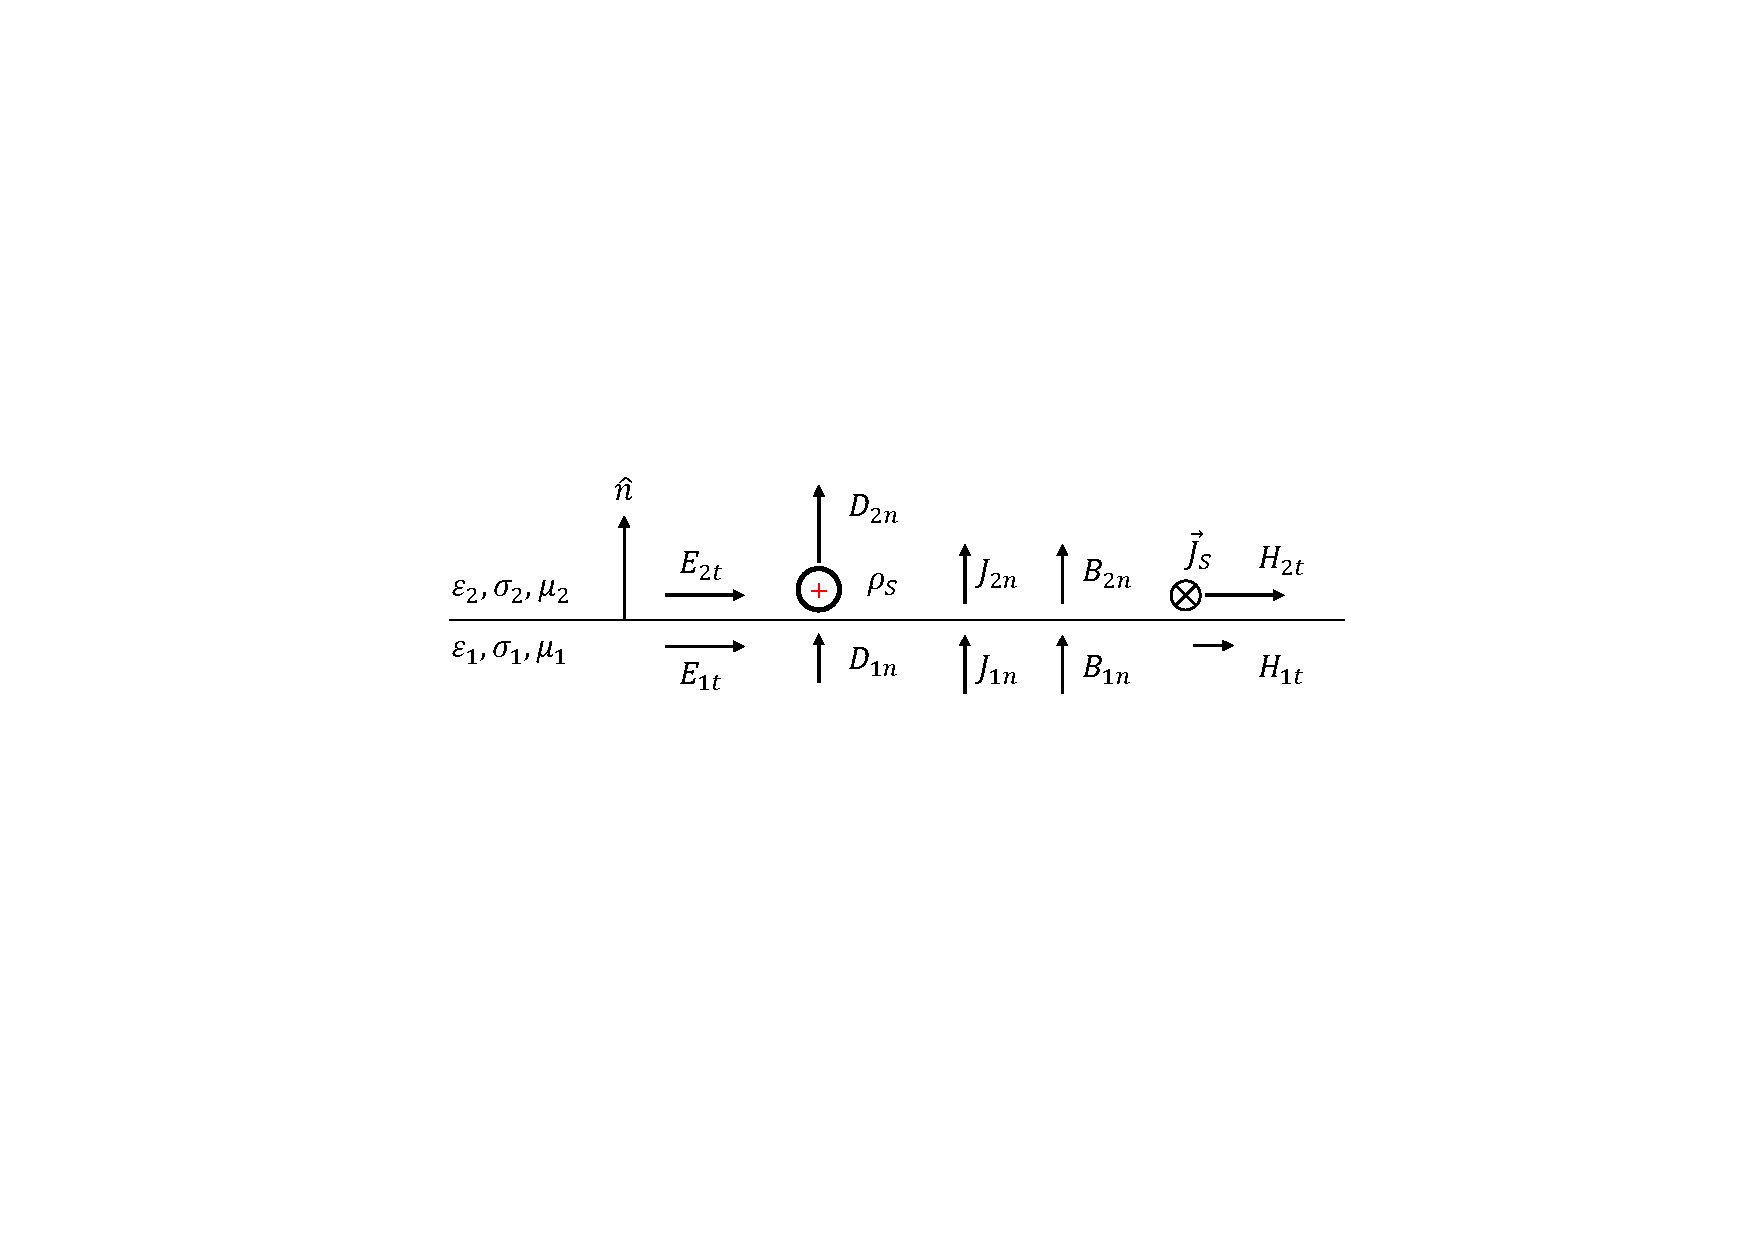
\includegraphics[width=10cm]{figure/5-1.pdf}
            \caption{\kaishu 一般介质界面边界条件示意图}\label{Fig: 介质边界条件示意图}
        \end{figure}

        特殊地,考虑两理想介质(1和2)的界面,以及理想导体(1)与理想介质(2)的界面处:
        \begin{subequations}
            \begin{numcases}{\mbox{理想介质1}\rightarrow\mbox{理想介质2}} 
                \hat{n}\cdot\left(\vec{D}_2-\vec{D}_1\right)=0\\
                \hat{n}\cdot\left(\vec{B}_2-\vec{B}_1\right)=0\\
                \hat{n}\times\left({\vec{E}}_2-{\vec{E}}_1\right)=0\\
                \hat{n}\times\left({\vec{H}}_2-{\vec{H}}_1\right)=0
            \end{numcases}
        \end{subequations}
        由此说明:两理想介质的界面处,电场、磁场沿任意方向连续;
        \begin{subequations}
            \begin{numcases}{\mbox{理想导体1}\rightarrow\mbox{理想介质2}} 
                \hat{n}\cdot\vec{D}_2=\rho_S\\
                \hat{n}\cdot\vec{B}_2=0\\
                \hat{n}\times{\vec{E}}_2=0\\
                \hat{n}\times{\vec{H}}_2=\vec{J}_S
            \end{numcases}
        \end{subequations}
        由此说明:PEC与理想介质的界面外部,电场垂直于界面,磁场平行于界面。


    \subsection{时谐电磁场的复矢量表示}
        {\color{gray}设正弦电场
        \begin{equation}
            \vec{E}=\vec{E}\left(x,y,z,t\right)=\left(E_x\left(x,y,z,t\right),E_y\left(x,y,z,t\right),E_z\left(x,y,z,t\right)\right)
        \end{equation}
        其每一个分量都是正弦量:
        \begin{equation}
            E_k\left(x,y,z,t\right)=E_{km}\left(x,y,z\right)\cos{\left(\omega t+\varphi_k\right)}
        \end{equation}
        其中$E_{km}$为空间一点的振幅在$\hat{k}$方向$(k=x,y,z)$上的分量,为实数。
        
        
        引入复振幅的好处在于,复振幅
        \begin{equation*}
            \dot{E}_{km}\left(x,y,z\right)=E_{km}\cdot \mathrm{e}^{\mathrm{j}(\omega t+\varphi_k)}
        \end{equation*}
        除了幅值外还可以表示电磁场的相位信息$\varphi_k$。由此,将原电场在$\hat{k}$方向上的分量作等量代换:
        \begin{equation}
            E_k\left(x,y,z\right)=\Re\left[{\dot{E}}_{km}\left(x,y,z\right)e^{\mathrm{j}\omega t}\right]
        \end{equation}
        原电场为
        \begin{equation}
            \vec{E}\left(x,y,z,t\right)=\Re\left[\left({\dot{E}}_{xm},{\dot{E}}_{ym},{\dot{E}}_{zm}\right)e^{\mathrm{j}\omega t}\right]
        \end{equation}
        又通常频率已经确定,省略掉$\cos{\omega t}$,则}定义电场强度的复矢量(in phasor form)为:
        \begin{equation}
            \dot{\vec{E}}(x,y,z)=\left({\dot{E}}_{xm},{\dot{E}}_{ym},{\dot{E}}_{zm}\right)
        \end{equation}
            其意义在于把时空的四维矢量函数简化成了空间的三维函数。


        复矢量表示下, 无源区域($\vec{J}=\vec{0},\,\rho=0$)  的麦克斯韦方程组变为:
        % \begin{subequations}
        %     \begin{numcases}{\mbox{}} 
        %         \nabla\times \dot{\bm{H}}=\mathrm{j}\omega \dot{\bm{D}} \\
        %         \nabla\times \dot{\bm{E}}=-\mathrm{j}\omega \dot{\bm{B}} \\
        %         \nabla\cdot \dot{\bm{B}}=0\\            
        %         \nabla\cdot \dot{\bm{D}}=0
        %     \end{numcases}
        % \end{subequations}
        
        \begin{subequations}
            \begin{align}
                &\nabla\times \dot{\vec{H}}=\mathrm{j}\omega \dot{\vec{D}} \\
                &\nabla\times \dot{\vec{E}}=-\mathrm{j}\omega \dot{\vec{B}} \\
                &\nabla\cdot \dot{\vec{B}}=0\\            
                &\nabla\cdot \dot{\vec{D}}=0
            \end{align}
        \end{subequations}


    \subsection{坡印廷定理}
        坡印亭(\emph{Pointing})定理:单位时间内输入一个闭合区域的的电磁能量,等于单位时间内区域内电场能量的增量,加上单位时间内区域的焦耳热。
        \begin{equation}
            -\oint_S\left(\vec{E}\times \vec{H}\right)\cdot \mathrm{d}\vec{S}
            =\frac{\partial }{\partial t}\int_V (\frac{1}{2}\vec{D}\cdot \vec{E}+\frac{1}{2}\vec{B}\cdot \vec{H})\,\mathrm{d}V
            +\int_V \vec{J}\cdot \vec{E}\,\mathrm{d}V
        \end{equation}

        定义坡印廷矢量$\vec{S}$(单位:\si{\watt\per\square\metre}):
        \begin{equation}
            \vec{S}=\vec{E}\times\vec{H}
        \end{equation}
        表示{\color{red}单位时间通过垂直单位面积的电磁能量},又称为{\color{red}电磁功率通量密度}。

        \vspace{5pt}
        \noindent\begin{boxedminipage}{\textwidth}
            \vspace{3pt}\setlength{\parindent}{2\ccwd}
            注意:$\oint_S \vec{S} \cdot \mathrm{d}\vec{S}$表示流出封闭曲面的总能流(单位:\si{\joule\per\second},也叫功率流,“流(flux)”强调该功率具有能速$\vec{v}_e=\frac{{\vec{S}}_{av}}{w_{av}}$),不能认为坡印廷矢量就代表电磁功率流密度。真正{\color{red}表示空间内一点功率流密度的是$\nabla\cdot \vec{S}$ } 而非$\vec{S}$本身。
            
            % {\color{gray}
            根据高斯定理有
            \begin{equation}
                \oint_S \vec{S} \cdot \mathrm{d}\vec{S}=\int_V \nabla\cdot \vec{S}\,\mathrm{d}V
            \end{equation}
            % }
            没有功率流动,说明无论闭合区域取多小,上积分式恒为0,即$\nabla·S=0$。说明这种情况下$\vec{S}$是一个旋度场,但并不一定有$\vec{S}=\vec{0}$。


            具体而言,在时变电磁场中,$\vec{S}$的物理意义表示电磁场的瞬时功率流密度,其曲面积分表示瞬时功率;但在静电场或静磁场中,$\vec{S}$并不代表功率流密度。
            {在静止的场中,没有功率的流动,能流密度不能代表功率的流动。}即虽然$\vec{S}\neq \vec{0}$但有$\nabla\cdot\vec{S}=0$
            \vspace{3pt}
        \end{boxedminipage}
        \vspace{5pt}


        定义平均坡印廷矢量(平均电磁功率通量密度):
        \begin{equation}
            {\vec{S}}_{av}=\frac{1}{T}\int_{0}^{T}{(\vec{E}\times\vec{H})\,\mathrm{d}t}=\frac{1}{2}\Re\left[\dot{\vec{E}}\times{\dot{\vec{H}}}^\ast\right]
        \end{equation}

    \subsection{波动方程}
        主要讨论均匀、线性,各向同性 介质的无源区域($\vec{J}=\vec{0},\,\rho=0$)内的情况。


        将介质的本构关系代入麦克斯韦方程组后,分别对第一、第二方程两边取旋度,利用矢量恒等式化简得:
        \begin{subequations}
            \begin{numcases}{\textbf{亥姆霍兹方程}} 
                \nabla^2  {\vec{E}}-\mu \varepsilon \frac{\partial^2  {\vec{E}}}{\partial t^2}=0 \\
                \nabla^2  {\vec{H}}-\mu \varepsilon \frac{\partial^2  {\vec{H}}}{\partial t^2}=0             
            \end{numcases}
        \end{subequations}
        可以将上式每个矢量方程分解为三个标量方程并求解,但这样很复杂。

        引入$\vec{E},\vec{H}$的复矢量,则 $\frac{\partial^2{\vec{E}}}{\partial t^2}=-\omega^2 \dot{\vec{E}}$,波动方程满足的偏微分方程变为:
        \begin{subequations}
            \begin{numcases}{\mbox{}} 
                \nabla^2\dot{\vec{E}}+ \omega^2 \mu \varepsilon \dot{\vec{E}}=0 \\
                \nabla^2\dot{\vec{H}}+ \omega^2 \mu \varepsilon \dot{\vec{H}}=0  
            \end{numcases}
        \end{subequations}
        并定义空间波数
        \begin{equation}
            k=\omega\sqrt{\mu \varepsilon}
        \end{equation}


\section{势函数及其解(矢位法)}
    通过求解辅助函数以得到电磁场,因此也称为辅助函数法。在微波/天线技术中,常用的辅助函数是\underline{矢量磁位}和\underline{标量电位},简称矢位和标位。

    \subsection{势函数及其规范}
        经典电动力学\footnote{不考虑Aharonov-Bohm效应(A-B效应),即认为磁场的物理效应可以完全用磁感应强度$\vec{B}$来描述,磁矢势$\vec{A}$不具有可观测的效应;也不考虑量子电动力学}所关心的是电荷的运动,而场作为一种物质其本身就是由它对其内电荷运动所产生的影响来刻画的(可以证明,验电荷在电磁场中的动能只与电荷量$e$,速度$\vec{v}$,以及电场磁场强度有关)。因此,如果两个电磁场能用同一组矢量$\vec{E}$和$\vec{B}$来表示,那么这两个场在物理上是全同的。
        % 电场和磁场是有物理意义的量,引入势函数仅仅是为了利于证明和计算。

        电场强度$\vec{E}$和磁感应强度$\vec{B}$只包含物理的自由度,即电磁场构型的每个自由度都对附近的验电荷的运动有单独可测量的效应。它们是关于势函数的单值函数:
        \begin{subequations}
            \begin{numcases}{\mbox{}} 
                \vec{E}=-\nabla \varphi-\frac{\partial \vec{A}}{\partial t}\\
                \vec{B}=\nabla\times\vec{A}
            \end{numcases}
        \end{subequations}
        
        但势函数除了包含物理自由度,还具有规范自由度,这是因为对于如下\textbf{势变换}:
        \begin{subequations}\label{Equ: 势变换}
            \begin{numcases}{\mbox{}} 
                \vec{A}\mapsto \vec{A}+\nabla \psi \\
                \varphi\mapsto \varphi-\frac{\partial \psi}{\partial t}
            \end{numcases}
            % \qquad $\psi(x,y,z;t)$为标量函数
        \end{subequations}

        电磁场的构型不变。即不同的势函数可以对应相同的电磁场。

        只有那些对于势变换\eqref{Equ: 势变换} 保持不变的量才有物理意义;特别是,所有方程在这个变换下必须是不变的。这种不变性称为\textbf{规范不变性}(德文为Eichinvarianz,英文为Gauge invariance)。


        因为势缺乏唯一性,我们就有可能去选择它们(即规范化:Guage fix),使它们满足我们所选择的附加条件。须指出,\underline{我们仅够令它们额外地满足一个标量等式}\footnote{这也解释了为什么库仑规范和洛伦兹规范只对磁矢势$\vec{A}$做出规定。因为引入一个关于$\vec{A}$的散度的标量方程后,$\varphi$也随之确定了},这是因为我们可以任意选择\eqref{Equ: 势变换}中的函数$\psi$。例如我们总可以选取合适的$\psi$,使得$\varphi=0$,即 Weyl gauge 。(但对于一个任意的$\vec{A}$,我们无法找到合适的$\psi$,使$\vec{A}=0$,因为这相当于引入了三个额外的条件。)除此之外还有 multipolar gauge,Fock Schwinger gauge, $R_\xi$ gauge 等等。

        其中常用的规范有库仑(Coulomb)规范和洛仑兹\footnote{是丹麦人ludvig Lorenz (1829—1891),在1867年提出了洛伦兹规范,并在前人基础上建立完善了滞后势:纽曼1845年在线圈互感的问题中提出了矢量势,黎曼可能在1857年左右得到了滞后势的概念,但是黎曼不幸去世,他的论文直到洛伦兹论文发表以后才出现。另一个洛伦兹是荷兰人Hendrik Lorentz (1853—1928),提出了相对论的洛伦兹变换。}(Lorenz)规范。

        \paragraph{库仑规范:}
        \begin{equation}
            \nabla\cdot\vec{A}=0
        \end{equation}
        库仑规范的优点是将麦克斯韦方程组关于电场的方程简化为静电场的形式:
        \begin{subequations}
            \begin{numcases}{\mbox{}} 
                \nabla^2 \varphi=-\frac{\rho}{\varepsilon}\label{Equ: 库仑规范下的第四方程}\\
                \nabla^2 \vec{A}=-\mu \vec{J}-\mu \varepsilon \frac{\partial \vec{E}}{\partial t}\label{Equ: 库仑规范下的第一方程}
            \end{numcases}
        \end{subequations}
            % 可以利用延迟格林函数,推迟势balabala,算出辐射的情况。

        {\color{gray}\begin{proof}
            将势函数与电场磁场的关系分别代入 第四方程 和 第一方程:
            \begin{equation*}
                \nabla\cdot\vec{E}
                =-\nabla^2 \varphi-\frac{\partial \left(\nabla\cdot\vec{A}\right)}{\partial t}
                =-\nabla^2 \varphi
                =\rho /\varepsilon
            \end{equation*}
            
            \begin{equation*}
                \nabla\times\vec{B}
                =\nabla\times \nabla\times\vec{A}=-\nabla^2 \vec{A}+\nabla \nabla\cdot\vec{A}
                =-\nabla^2 \vec{A}
                =\mu \left(\vec{J}+\frac{\partial \vec{D}}{\partial t}\right)
            \end{equation*}
        \end{proof}}

        得到的方程组中,电标位很好求:\hyperref[Equ: 库仑规范下的第四方程]{式(\ref*{Equ: 库仑规范下的第四方程})}正是静电场的泊松方程,它的解为:
        \begin{equation}
            \varphi(\vec{r},t)=\frac{1}{4\pi \varepsilon}\int\limits_V \frac{\rho(\vec{r}',t)}{|\vec{r}-\vec{r}'|}\,\mathrm{d}V'+\mathrm{const}
        \end{equation}
        这是体分布的电荷在场点$\vec{r}$处的电位,为了方便常取$\mathrm{const}=0$。若为面电荷或线电荷,则改变积分区域和微分单元即可。

        但是磁矢位满足的方程\eqref{Equ: 库仑规范下的第一方程},麦克斯韦自己也没有办法求解,只能考虑没有位移电流的特殊情况。所以麦克斯韦从来没有得到过像洛伦兹那样的滞后势解(即\hyperref[Equ: 滞后势的解]{式(\ref*{Equ: 滞后势的解})})。

        在无位移电流的情况(静电场)下,磁矢位满足的方程\eqref{Equ: 库仑规范下的第一方程}变为
        \begin{equation}
            \nabla^2 \vec{A}=-\mu \vec{J}
        \end{equation}
        只需类比泊松方程的解,得到
        \begin{equation}
            \vec{A}(\vec{r},t)=\frac{\mu}{4\pi}\int\limits_V \frac{\vec{J}(\vec{r}',t)}{|\vec{r}-\vec{r}'|}\,\mathrm{d}V'
        \end{equation}

        由此可见,库仑规范下认为电荷分布产生了势$\varphi$,电流分布产生了磁矢势$\vec{A}$,因果关系明了,且具有瞬态性(instantaneous)。
        
        缺点除了磁矢势不方便求解,还有不满足洛伦兹协变性(Lorentz invariance),在和狭义相对论结合的时候会出问题。
        
        \paragraph{洛伦兹规范}
        \begin{equation}
            \nabla\cdot\vec{A}+\mu \varepsilon\frac{\partial \varphi}{\partial t}=0
        \end{equation}
        % \begin{equation}
        %     \nabla\cdot\vec{A}+\frac{1}{c^2}\frac{\partial \varphi}{\partial t}=0
        % \end{equation}
        
        利用洛伦兹规范,则可以通过麦克斯韦方程组求解出势函数,过程如下:
        
        用辅助矢位和标位函数表示待求场矢量:
        \begin{subequations}
            \begin{numcases}{\mbox{}} 
                \vec{E}=-\nabla \varphi-\frac{\partial \vec{A}}{\partial t}\label{Equ: 辅助函数表示电场} \\
                \vec{H}=\frac{1}{\mu}\left(\nabla\times\vec{A}\right)
            \end{numcases}
        \end{subequations}
        代入第一方程,得:
        \begin{equation}
            \nabla\times \frac{1}{\mu}\nabla\times\vec{A}=\vec{J}+\varepsilon \frac{\partial }{\partial t}\left(-\nabla \varphi-\frac{\partial \vec{A}}{\partial t}\right)
        \end{equation}
        再将洛伦兹规范代入上式,化简得:
        \begin{subequations}\label{Equ: 辅助函数的达朗贝尔方程}
        \begin{equation}\label{Equ: 辅助函数的达朗贝尔方程A}
            \nabla^2 \vec{A}-\mu \varepsilon \frac{\partial^2 \vec{A}}{\partial t^2}=-\mu \vec{J}
        \end{equation}
        同理,将\hyperref[Equ: 辅助函数表示电场]{式(\ref*{Equ: 辅助函数表示电场})}和洛仑兹规范代入第四方程,可以得:
        \begin{equation}\label{Equ: 辅助函数的达朗贝尔方程phi}
            \nabla^2 \varphi-\mu \varepsilon \frac{\partial^2 \varphi}{\partial t^2}=-\frac{\rho}{\varepsilon}
        \end{equation}
        \end{subequations}
        \hyperref[Equ: 辅助函数的达朗贝尔方程A]{式(\ref*{Equ: 辅助函数的达朗贝尔方程A})}和\hyperref[Equ: 辅助函数的达朗贝尔方程phi]{式(\ref*{Equ: 辅助函数的达朗贝尔方程phi})}的形式相同,这种形式的波动方程称为\textbf{达朗贝尔方程}。

        达朗贝尔方程的标量形式可用格林定理求解,其解为:
        \begin{subequations}\label{Equ: 滞后势的解}
            \begin{numcases}{\mbox{}} 
                \vec{A}(\vec{r},t)=\frac{\mu}{4\pi}\int\limits_V \frac{\vec{J}(\vec{r}',t)\mathrm{e}^{-\mathrm{j}k|\vec{r}-\vec{r}'|}}{|\vec{r}-\vec{r}'|}\,\mathrm{d}V'\\
                \varphi(\vec{r},t)=\frac{1}{4\pi \varepsilon}\int\limits_V \frac{\rho(\vec{r}',t)\mathrm{e}^{-\mathrm{j}k|\vec{r}-\vec{r}'|}}{|\vec{r}-\vec{r}'|}\,\mathrm{d}V'
            \end{numcases}
        \end{subequations}
        其中$k=\omega\sqrt{\mu \varepsilon}$。
        
        \paragraph{规范化的实质和意义}
        ~\\ \vspace{-5pt}% 首先应指出,只有在经典动力学中,规范化才是不唯一的。
        
        满足势变换\eqref{Equ: 势变换}的两组不同的势函数其实对应同一个物理体系:它们是同一个电磁场的不同解。解不同的本质原因在于参照系不同。设想有一个理想的圆柱,如果被扭了但又保持圆柱的形状,你当然无法知道是否发生扭曲了。但是,若在圆柱的底端到顶端加一条曲线,则从曲线的变化可以判断是否发生了扭曲。这个过程就是一个 gauge fixing 的过程。规范化其说是添加约束,更准确地说是添加参照。注意,这条曲线是从外部加上去的,不属于考察的对象,因此也不应该影响考察对象的性质。

        {\color{gray}
            从数学的角度上,由于已经满足$\nabla\times\vec{A}=\vec{B}$,那么根据亥姆霍兹定理,唯一确定场矢量$\vec{A}$只需要再确定$\vec{A}$的散度即可。因此规范化的目的是为了求得唯一的磁矢势$A$。但是这种看法似乎认为是先给出$\vec{B}$,再求$\vec{A}$,而实际上物理学观点认为是先有磁矢势,再有磁场强度。
        }

        在求解经典电动力学的问题时,可以因具体问题的的方便程度人为选取一个gauge fix,选取得适当则可以使问题大大简化。


    \subsection{滞后势的求解}
        滞后势,即引入了矢量位和标量位来描述电磁场后,\underline{洛伦兹规范}下求得的磁矢势$\vec{A}$和电势$\varphi$。“滞后”体现在从源点$\vec{r}'$作用到场点$\vec{r}$,需要延迟$\frac{|\vec{r}-\vec{r}'|}{v}$的时间。换句话说,场点位函数的变化始终滞后于场源的变化,滞后的时间就是电磁波传播距离$R=|\vec{r}-\vec{r}'|$所需要的时间。(这与库伦规范下的势函数解具有瞬时性恰好矛盾)

        \begin{lemma}{格林定理}{格林定理}
            $u,w$为任意标量函数,且$u,w$以及它们的一阶、二阶导数在$V$内连续,则
            \begin{equation}
                \int\limits_V (u \nabla^2w-w \nabla^2u)\,\mathrm{d}V=\oint\limits_S (u \nabla w-w \nabla u)\cdot\mathrm{d}\vec{S}
            \end{equation}
        \end{lemma}

        令其中$u=\varphi,\;w=\psi=\frac{\mathrm{e}^{-\mathrm{j}k R}}{R}$,则在$V$内除$R=0\,(\vec{r}'=\vec{r})$外的区域,$\psi$符合格林定理中标量函数的约束条件。不妨假设$\varphi$也在该区域内符合条件。

        为了排除被积函数的奇点(不让积分变点$\vec{ r}'$取到场点$\vec{r}$),则以场点$\vec{r}$为圆心,作一半径为$a$的小球,其表面为$S_2$,体积为$V_2$。于是积分体积变为$V_1=V-V_2$,积分表面变为$S_1=S+S_2$。

        由格林定理:
        \begin{equation}\label{Equ: 方程求解滞后势}
            \int\limits_{V_1}\left[\varphi \nabla^2\psi-\psi \nabla^2 \varphi\right]\,\mathrm{d}V'
            =\oint\limits_{S} \left[\varphi \frac{\partial \psi}{\partial \hat{n}}-\psi \frac{\partial \varphi}{\partial \hat{n}}\right]\cdot\mathrm{d}\vec{S}'
            +\oint\limits_{S_2} \left[\varphi \frac{\partial \psi}{\partial \hat{n}}-\psi \frac{\partial \varphi}{\partial \hat{n}}\right]\cdot\mathrm{d}\vec{S}'
        \end{equation}
        这里用到了恒等式
        \begin{equation*}
            \nabla \varphi \cdot \hat{n}\mathrm{d}S
            =\left(\frac{\partial \varphi}{\partial x}\hat{x}+\frac{\partial \varphi}{\partial y}\hat{y}+\frac{\partial \varphi}{\partial z}\hat{z}\right)\cdot \mathrm{d}\vec{S}
            =\frac{\partial \varphi}{\partial \hat{n}}\cdot \mathrm{d}\vec{S}
            =\frac{\partial \varphi}{\partial n}\mathrm{d}S
        \end{equation*}
        其中$\frac{\partial \varphi}{\partial n}$即$\varphi$沿$\hat{n}$方向的方向导数,也等于此处电场沿$\hat{n}$方向的分量的相反数。

        注意到,积分变点$\vec{r}'\in S_2$时,$\hat{n}$($\mathrm{d}\vec{S}$)恒指向小球球心,其方向与变量$R$增大的方向相反,因此$\frac{\partial \;\cdot }{\partial n}=-\frac{\partial \;\cdot}{\partial R}$。
        
        且有立体角元定义
        \begin{equation}
            \mathrm{d}\varOmega=\frac{\mathrm{d}A}{r^2}=\sin\theta \,\mathrm{d}\theta \,\mathrm{d}\phi
        \end{equation}
        
        因此
        \begin{equation*}
            \begin{aligned}
                \oint\limits_{S_2} \left[\varphi \frac{\partial \psi}{\partial \hat{n}}-\psi \frac{\partial \varphi}{\partial \hat{n}}\right]\cdot\mathrm{d}\vec{S}'
                &=\oint\limits_{S_2} \left[-\varphi \frac{\partial \psi}{\partial R}+\psi \frac{\partial \varphi}{\partial R}\right]_{R=a} \,a^2\mathrm{d}\varOmega'\\
                &=\oint\limits_{S_2} \left[-\varphi \left(-\frac{1}{R^2}-\frac{\mathrm{j}k}{R}\right)\mathrm{e}^{-\mathrm{j}k R}+ \frac{\mathrm{e}^{-\mathrm{j}kR}}{R} \frac{\partial \varphi}{\partial R}\right]_{R=a} \,a^2\mathrm{d}\varOmega'\\
                &=\oint\limits_{S_2} \left[\left.\varphi(\vec{r}')\right\vert_{R=a} \left(1+\mathrm{j}ka\right)\mathrm{e}^{-\mathrm{j}ka}+ a\mathrm{e}^{-\mathrm{j}ka}\left.\frac{\partial \varphi}{\partial R}\right\vert_{R=a}\right] \,\mathrm{d}\varOmega'
            \end{aligned}
        \end{equation*}

        由于$\varphi, \frac{\partial \varphi}{\partial R}$均有限,上式在$a\rightarrow 0$时将收敛于:
        \begin{equation*}
            \lim_{a \to 0}{\oint\limits_{S_2} \left[\varphi \frac{\partial \psi}{\partial \hat{n}}-\psi \frac{\partial \varphi}{\partial \hat{n}}\right]\cdot\mathrm{d}\vec{S}'}
            =\lim_{a \to 0}{\oint\limits_{S_2}\left.\varphi(\vec{r}')\right\vert_{R=a}\,\mathrm{d}\varOmega'}
            =\varphi(\vec{r})\oint\limits_{S_2}\,\mathrm{d}\varOmega'
            =4\pi\varphi(\vec{r})
        \end{equation*}
        后两个等号成立是因为,小球无限缩小时$\left.\varphi(\vec{r}')\right\vert_{R=a}$可用球心处的电势$\varphi(\vec{r})$代替,且所有封闭曲面内的立体角元积分均为$\int_{0}^{\pi}\int_{0}^{2\pi}\sin\theta \,\mathrm{d}\theta \,\mathrm{d}\phi=4\pi$。

        将上式极限$a\rightarrow 0$时的结论代入到方程(\eqref{Equ: 方程求解滞后势})中,得:
        \begin{equation}
            \begin{aligned}
                \varphi(\vec{r})
                &=\frac{1}{4\pi}\lim_{a \to 0}\left\{\int\limits_{V_1}\left[\varphi \nabla^2\psi-\psi \nabla^2 \varphi\right]\,\mathrm{d}V'
                -\oint\limits_{S} \left[\varphi \frac{\partial \psi}{\partial \hat{n}}-\psi \frac{\partial \varphi}{\partial \hat{n}}\right]\cdot\mathrm{d}\vec{S}'\right\}\\
                &=\frac{1}{4\pi}\left\{\int\limits_{V}\left[\varphi \nabla^2\psi-\psi \nabla^2 \varphi\right]\,\mathrm{d}V'
                -\oint\limits_{S} \left[\varphi \frac{\partial \psi}{\partial \hat{n}}-\psi \frac{\partial \varphi}{\partial \hat{n}}\right]\cdot\mathrm{d}\vec{S}'\right\}\\
            \end{aligned}
        \end{equation}

        注意到在时谐场的条件下,$\varphi$和$\psi$都满足亥姆霍兹方程:
        \begin{subequations}
            \begin{numcases}{\mbox{}} 
                \nabla^2\psi+k^2\psi=0\\
                \nabla^2 \varphi+k^2 \varphi=-\frac{\rho}{\varepsilon}
            \end{numcases}
        \end{subequations}

        将$\nabla^2 \varphi$和$\nabla^2\psi$代入化简,得:
        \begin{equation}\label{Equ: 亥姆霍兹积分}
            \begin{aligned}
                \varphi(\vec{r})
                &=\frac{1}{4\pi}\left\{\int\limits_{V}\psi \frac{\rho(\vec{r}')}{\varepsilon}\,\mathrm{d}V'
                -\oint\limits_{S} \left[\varphi \frac{\partial \psi}{\partial n}-\psi \frac{\partial \varphi}{\partial n}\right]\,\mathrm{d}S'\right\}\\
                &=\frac{1}{4\pi \varepsilon}\int\limits_{V}\psi \rho(\vec{r}')\,\mathrm{d}V'
                -\frac{1}{4\pi}\oint\limits_{S} \left[\varphi \frac{\partial \psi}{\partial n}-\psi \frac{\partial \varphi}{\partial n}\right]\,\mathrm{d}S' % \\
                % &=\frac{1}{4\pi \varepsilon}\int\limits_{V}\frac{\rho(\vec{r}')\mathrm{e}^{-\mathrm{j}kR}}{R}\,\mathrm{d}V'
                % -\frac{1}{4\pi}\oint\limits_{S} \left[\varphi(\vec{r}') \frac{\partial}{\partial n}\left(\frac{\mathrm{e}^{-\mathrm{j}kR}}{R}\right)-\frac{\partial \varphi(\vec{r}')}{\partial n}\frac{\mathrm{e}^{-\mathrm{j}kR}}{R}\right]\,\mathrm{d}S'
            \end{aligned}
        \end{equation}

        同理构造标量函数$\psi$结合格林定理,可以解出磁矢势。至此,我们已经求解出了洛伦兹规范下满足时谐场条件的滞后势:
        \begin{subequations}\label{Equ: 滞后势的初始解}
            \begin{numcases}{\mbox{}} 
                \varphi(\vec{r})
                =\frac{1}{4\pi \varepsilon}\int\limits_{V}\frac{\rho(\vec{r}')\mathrm{e}^{-\mathrm{j}kR}}{R}\,\mathrm{d}V'
                -\frac{1}{4\pi}\oint\limits_{S} \left[\varphi(\vec{r}') \frac{\partial}{\partial n}\left(\frac{\mathrm{e}^{-\mathrm{j}kR}}{R}\right)-\frac{\partial \varphi(\vec{r}')}{\partial n}\frac{\mathrm{e}^{-\mathrm{j}kR}}{R}\right]\,\mathrm{d}S'\\
                \vec{A}(\vec{r})
                =\frac{\mu}{4\pi}\int\limits_{V}\frac{\vec{J}(\vec{r}')\mathrm{e}^{-\mathrm{j}kR}}{R}\,\mathrm{d}V'
                -\frac{1}{4\pi}\oint\limits_{S} \left[\vec{A}(\vec{r}') \frac{\partial}{\partial n}\left(\frac{\mathrm{e}^{-\mathrm{j}kR}}{R}\right)-\frac{\partial \vec{A}(\vec{r}')}{\partial n}\frac{\mathrm{e}^{-\mathrm{j}kR}}{R}\right]\,\mathrm{d}S'
            \end{numcases}
        \end{subequations}
        该结论首先由亥姆霍兹得出,故称形如\hyperref[Equ: 亥姆霍兹积分]{式(\ref*{Equ: 亥姆霍兹积分})}的积分式为亥姆霍兹积分。

        结果表明,空间中的滞后势由两部分场源贡献:体积分的部分表示体积$V$内的源,闭合面$S$上的积分表示$V$外场源的贡献。

    \subsection{辐射条件}
        在考虑无限空间中的电磁问题时,设积分曲面$S$为半径$R$的球面。由于\hyperref[Equ: 滞后势的初始解]{式(\ref*{Equ: 滞后势的初始解})}中面积分的单位矢量$\hat{n}$指向$R$增大的方向,有$\frac{\partial \;\cdot}{\partial n}=\frac{\partial \;\cdot}{\partial R}$,可以将面积分写为:
        \begin{equation*}
            -\frac{1}{4\pi} \oint\limits_S \left[\varphi(\vec{r}')\left(-\frac{1}{R^2}-\frac{\mathrm{j}k}{R}\right)\mathrm{e}^{-\mathrm{j}k R} - \frac{\partial \varphi(\vec{r}')}{\partial R} \frac{\mathrm{e}^{-\mathrm{j}kR}}{R}\right] \mathrm{d}S'
        \end{equation*}
        再使用立体角代换$\mathrm{d}S'=R^2 \mathrm{d}\varOmega'$,面积分等价于:
        \begin{equation}
            \frac{1}{4\pi} \oint\limits_S \left[\varphi(\vec{r}')\left(1+\mathrm{j}kR\right)\mathrm{e}^{-\mathrm{j}k R} + R\frac{\partial \varphi(\vec{r}')}{\partial R} \mathrm{e}^{-\mathrm{j}kR}\right] \mathrm{d}\varOmega'
        \end{equation}

        为了排除无限远处的场源,就要使无限远处场源的积分贡献为0,也就是要使上式面积分为0结果。
        
        则得到辐射条件:
        \begin{subequations}
            \begin{numcases}{} 
                \mbox{电标位的辐射条件:}\lim_{R \to \infty}{R\left(\frac{\partial \varphi(\vec{r}')}{\partial R}+\mathrm{j}k \varphi(\vec{r}')\right)}=0\\
                \mbox{磁矢位的辐射条件:}\lim_{R \to \infty}{R\left(\frac{\partial \vec{A}(\vec{r}')}{\partial R}+\mathrm{j}k \vec{A}(\vec{r}')\right)}=0
            \end{numcases}
        \end{subequations}

        辐射条件的本质是:要求 \underline{场源产生的滞后势在远离场源的空间中至少要以$R^{-1}$的速度衰减}。

        满足辐射条件的滞后势简化为:
        \begin{subequations}\label{Equ: 辐射场的滞后势解}
            \begin{numcases}{\mbox{}} 
                \varphi(\vec{r})
                =\frac{1}{4\pi \varepsilon}\int\limits_{V}\frac{\rho(\vec{r}')\mathrm{e}^{-\mathrm{j}kR}}{R}\,\mathrm{d}V'\\
                \vec{A}(\vec{r})
                =\frac{\mu}{4\pi}\int\limits_{V}\frac{\vec{J}(\vec{r}')\mathrm{e}^{-\mathrm{j}kR}}{R}\,\mathrm{d}V'
            \end{numcases}
        \end{subequations}

\section{电基本振子}

        电基本振子,或称为\emph{电偶极子天线}, 是一段载有高频电流的线元。其长度$\Delta  l\ll \lambda$,故认为其上各点电流振幅相同,相位相同。

    \subsection{电基本振子的辐射场}
        设电流元沿$\hat{z}$方向。根据辐射条件下的磁矢位解,有
        \begin{equation}
            \begin{aligned}
                \vec{A}(\vec{r})&=\frac{\mu}{4\pi}\int\limits_{V}\frac{\vec{J}(\vec{r}')\mathrm{e}^{-\mathrm{j}kR}}{R}\,\mathrm{d}V'\\
                &=\frac{\mu}{4\pi}\int\limits_{l}\frac{I\hat{z}}{\Delta S}\frac{\mathrm{e}^{-\mathrm{j}kR}}{R}\,\Delta S\mathrm{d}l'\\
                &=\frac{\mu}{4\pi}\frac{\mathrm{e}^{-\mathrm{j}kr}}{r}\int\limits_{l}I\hat{z}\,\mathrm{d}l'\qquad\mbox{\color{gray}$(\Delta l\ll R)$}\\
                &=\frac{\mu I \Delta l}{4\pi r}\mathrm{e}^{-\mathrm{j}kr}\hat{z}
            \end{aligned}
        \end{equation}
        注意,当$\vec{J}(\vec{r}')$为复矢量时,$I$为复数(电流相量):$\dot{I}=\dot{I}_m \mathrm{e}^{\mathrm{j}\varphi_{I0}}=I_m\cos(\omega t+\varphi_{I0})$省略上标$\dot{~}$的形式。

        使用相量表示电压电流,则
        \begin{equation}
            Q=\frac{I}{\mathrm{j}\omega}
        \end{equation}
        表示电流元两端聚积的大小相等,符号相反的时谐电荷量。

        {\color{gray} 由此可以求得标量电位
        \begin{equation}
            \begin{aligned}
                \varphi(\vec{r})
                &=\frac{1}{4\pi \varepsilon}\int\limits_{V}\frac{\rho(\vec{r}')\mathrm{e}^{-\mathrm{j}kR}}{R}\,\mathrm{d}V'\\
                &=\frac{1}{4\pi \varepsilon}\int\limits_{l}\frac{\frac{Q}{\Delta S \mathrm{d}l}\mathrm{e}^{-\mathrm{j}kR}}{R}\, \Delta S\mathrm{d}l'\\
                &=\frac{Q}{4\pi \varepsilon r}\mathrm{e}^{-\mathrm{j}kr}
            \end{aligned}
        \end{equation}
        }

        引入球坐标系以便于研究电基本振子的辐射场:
        \begin{equation}
            \vec{A}=\hat{r}A_r+\hat{\theta}A_\theta+\hat{\phi}A_\phi=\hat{r}A_z\cos\theta-\hat{\theta}A_z\sin\theta
        \end{equation}
        其中$\hat{\theta}$前的负号是由于$\hat{z}A_z$在沿$\hat{r}$和$\hat{\theta}$正交分解时,$A_\theta$分量的方向与$\hat{\theta}$增大的方向相反。

        由$\vec{A}$表示磁场:
        \begin{equation}
            \begin{aligned}
                \vec{H}(\vec{r})=\frac{1}{\mu}\nabla\times \vec{A}
                =\frac{1}{\mu r^2\sin\theta}\begin{vmatrix}
                    \hat{r}&r\hat{\theta}&r\sin\theta\hat{\phi}\\
                    \frac{\partial }{\partial r}&\frac{\partial }{\partial \theta}&\frac{\partial }{\partial \phi}\\
                    A_z\cos\theta&-rA_z\sin\theta&0
                \end{vmatrix}
            \end{aligned}
        \end{equation}

        再由麦克斯韦方程组第一方程,$\vec{E}=\frac{1}{\mathrm{j}\omega \varepsilon}\nabla\times \vec{H}$,可以解出电基本振子的辐射场:

        \begin{equation}\label{Equ: 电基本振子的辐射场}
            \begin{array}{l c cc cc}
                \vec{H}=&\hat{r}0 &+&\hat{\theta}0&+&\hat{\phi}\frac{I \mathrm{d}l\sin\theta}{4\pi}\left[\frac{\mathrm{j}k}{r}+\frac{1}{r^2}\right]\mathrm{e}^{-\mathrm{j}k r}\\
                \vec{E}=&\hat{r}\frac{2I \mathrm{d}l\cos\theta}{4\pi \varepsilon \mathrm{j}\omega}\left[\frac{\mathrm{j}k}{r^2}+\frac{1}{r^3}\right]\mathrm{e}^{-\mathrm{j}k r} &+&\hat{\theta}\frac{I \mathrm{d}l\sin\theta}{4\pi \varepsilon \mathrm{j}\omega}\left[-\frac{k^2}{r}+\frac{\mathrm{j}k}{r^2}+\frac{1}{r^3}\right]\mathrm{e}^{-\mathrm{j}k r}&+&\hat{\phi}0\\
            \end{array}
        \end{equation}

    \subsection{电基本振子的近、远场辐射特性}
        从电基本振子的辐射场\hyperref[Equ: 电基本振子的辐射场]{式(\ref*{Equ: 电基本振子的辐射场})}可以看出,电磁场强度的幅度是$r$的函数,随距离增大以不同的速度衰减。

        以此把辐射场划分为近场区和远场区:
        \begin{itemize}
            \item 近场区:$\frac{1}{r^3}\gg\frac{k}{r^2}\gg\frac{k^2}{r}$。电场近似为只含有$\frac{1}{r^3}$分量,磁场近似为只含有$\frac{k}{r^2}$分量。
            \item 远场区:$\frac{1}{r^3}\ll\frac{k}{r^2}\ll\frac{k^2}{r}$。电磁场都只考虑$\frac{k^2}{r}$分量。
        \end{itemize}
        对于其他各种天线,判断近场远场通常用以下经验公式:
        \begin{itemize}
            \item 近场区:取$r<3 \lambda$。
            \item 远场区:对电大尺寸天线,取距离不至于使源到天线边缘与到天线中央的波程差小于$\frac{\pi}{8}/\beta$。对电小尺寸天线,取$r>10 \lambda$。
                \begin{equation}
                    r>
                    \left\{\begin{aligned}
                        &\frac{2D^2}{\lambda}\;,\quad \mbox{电大尺寸}\\
                        &10 \lambda\;,\quad \mbox{电小尺寸}
                    \end{aligned}\right.
                \end{equation}
        \end{itemize}

        \paragraph*{近场区的辐射特性}
        根据以上近似,计算近场区辐射场的复坡印廷矢量:
        \begin{equation}
            \vec{S}
            = \frac{1}{2}\left[\hat{r}E_\theta H_\phi^*-\hat{\theta}E_r H_\phi^*\right]
            % \vec{S}_{av}=\frac{1}{2}\Re\left[\vec{E}\times \vec{H}^*\right]=\frac{1}{2}\Re\left[\hat{r}E_\theta H_\phi^*-\hat{\theta}E_r H_\phi^*\right]
        \end{equation}
        只含有虚部,这说明近场区几乎只存在电场与磁场的能量交换,而少有能量辐射出来。因此近场区也叫感应区,这样的辐射场为感应场。

        \paragraph*{远场区的辐射特性}
        远场区只考虑了$\frac{k^2}{r}$分量,此时
        \begin{subequations}
            \begin{numcases}{\mbox{远场区辐射场}} 
                \begin{aligned}
                    \vec{E}
                    &\approx \hat{\theta}E_\theta\\
                    &\approx \hat{\theta}\mathrm{j}\frac{I \Delta z \eta}{2 \lambda r}\sin\theta \mathrm{e}^{-\mathrm{j}k r}
                \end{aligned}\\
                \begin{aligned}
                    \vec{H}
                    &\approx \hat{\phi}H_\phi\\
                    &\approx \hat{\phi}\mathrm{j}\frac{I \Delta z}{2 \lambda r}\sin\theta \mathrm{e}^{-\mathrm{j}k r}
                \end{aligned}
            \end{numcases}
        \end{subequations}

        计算远场区辐射场的复坡印廷矢量
        \begin{equation}\label{Equ: 电基本振子远场区的功率通量密度}
            \vec{S}
            \approx \frac{1}{2}\hat{r}E_\theta H_\phi^*
            \approx \hat{r} \tikzmarknode{Poynting}{\highlight{red}{$\frac{|I \Delta z|^2\eta}{8 \lambda^2 r^2}\sin^2\theta$}}
        \end{equation}
        \begin{tikzpicture}[overlay,remember picture,>=stealth,nodes={align=left,inner ysep=1pt},<-]
        \path (Poynting.north) ++ (0,1.5em) node[anchor=south west,color=red!67] (annotation1){\textbf{功率通量密度$\vec{S}_r(\theta,\phi)$}};
        \draw [color=red!57](Poynting.north) |- ([xshift=-0.3ex,color=red]annotation1.south east);
        \end{tikzpicture}
        只有实部,向外辐射能量。并且具有类似平面波的特征:$|\vec{S}|=\frac{|E_\mathrm{m}|^2}{2\eta}$。
        
        如果电流元沿地轴放置,那么远场区场分布的特点:电场沿经线方向、磁场沿纬线方向。
        
    % \subsection{电基本振子的远场区}
    

% !TeX root = Microwave.tex
\chapter{天线的电参数}
\begin{equation*}
\mbox{天线参数}
\begin{cases}
    \mbox{电路参量}
    \begin{cases}
        \mbox{天线阻抗}\\
        \mbox{辐射电阻}
    \end{cases}\\
    \mbox{空间参量}
    \begin{cases}
        \mbox{场波瓣图}\\
        \mbox{功率波瓣图}\\
        \mbox{定向性}D\\
        \mbox{增益}G\\
        \mbox{极化}\mathrm{LP},\mathrm{CP},\mathrm{EP}
    \end{cases}
\end{cases}
\end{equation*}

\section{辐射特性参数}
    辐射特性有功率通量密度$\vec{S}(\theta,\phi)$(Power flux density)、辐射强度$P_r(\theta,\phi)$(Radiation intensity)、场强(Fields strength)、相位(Phase)、极化(Polarization)等;

    \subsection{辐射方向图}
    天线的辐射方向图一般描述天线在远场区的辐射特性。
    \begin{definition}
    {辐射方向图(Radiation Pattern)}
    {辐射方向图}
    天线的辐射特性是关于空间坐标的函数,若在\textbf{固定距离}上,此函数通过数学函数或者图形来描述,则得到的数学函数或者图形即为辐射方向图(Radiation Pattern),简称方向图。
    \tcblower
    通常而言,这里的辐射特性指电场强度,空间坐标表示为$(\theta,\phi)$。则天线的方向图定义为
    \begin{equation}
        f(\theta,\phi)=\frac{|\vec{E}(\theta,\phi)|}{A_0}
    \end{equation}
    其中$A_0$是$|\vec{E}(\theta,\phi)|$表达式中与$\theta,\phi$无关的因式。
    
    这种定义又叫 Field Amplitude Pattern,区别于 Power Pattern。
    \end{definition}    
    

    \begin{definition}
    {归一化方向图}
    {归一化方向图}
        定义天线的归一化场强方向图为$F(\theta,\phi)$:
        \begin{equation}
            F(\theta,\phi)
            =\frac{f(\theta,\phi)}{f_\mathrm{max}}
            =\frac{|E(\theta,\phi)|}{E_\mathrm{m}}
        \end{equation}
        则天线的归一化功率方向图可以表示为$F^2(\theta,\phi)$。
    \end{definition}


        
        方向图中主要关注的参数:
        \begin{enumerate}
            \item 零功率波瓣宽度(FNBW) $2\theta_{OE}$ 和 $2\theta_{OH}$:指主瓣最大值两边两个零辐射方向的夹角。
            \item 半功率波瓣宽度(HPBW) $2\theta_{OE}$ 和 $2\theta_{OE}$:指主瓣最大值两边功率通量密度下降到最大值的一半(或场强下降到最大值的0.707)时,即下降\SI{3}{\decibel}的两点间的夹角。
            \item 旁瓣电平(FSLL):指第一旁瓣功率密度和主瓣功率密度之比的对数值
                \begin{equation}
                    \xi_1=10\lg\frac{S(\theta_1,\varphi_1)}{S} 
                \end{equation}
            副瓣方向通常是不需要辐射或接收能量的方向。因此,天线副瓣电平越低,表明天线在不需要方向上辐射或接收的能量越弱,或者说在这些方向上对杂散的来波抑制能力越强,抗干扰能力就越强。因此,在天线设计中常有低副瓣设计要求。如基站的上旁瓣、雷达天线。
            
            \item 前后抑制比 $\xi_b$:后瓣最大辐射方向上功率密度和主瓣功率密度之比的对数值。
                \begin{equation}
                    \xi_b=10\lg\frac{S_b}{S_M}=20\lg\frac{|E_b|}{|E_M|}
                \end{equation}
        \end{enumerate}

        \begin{figure}[htp]
            \centering
            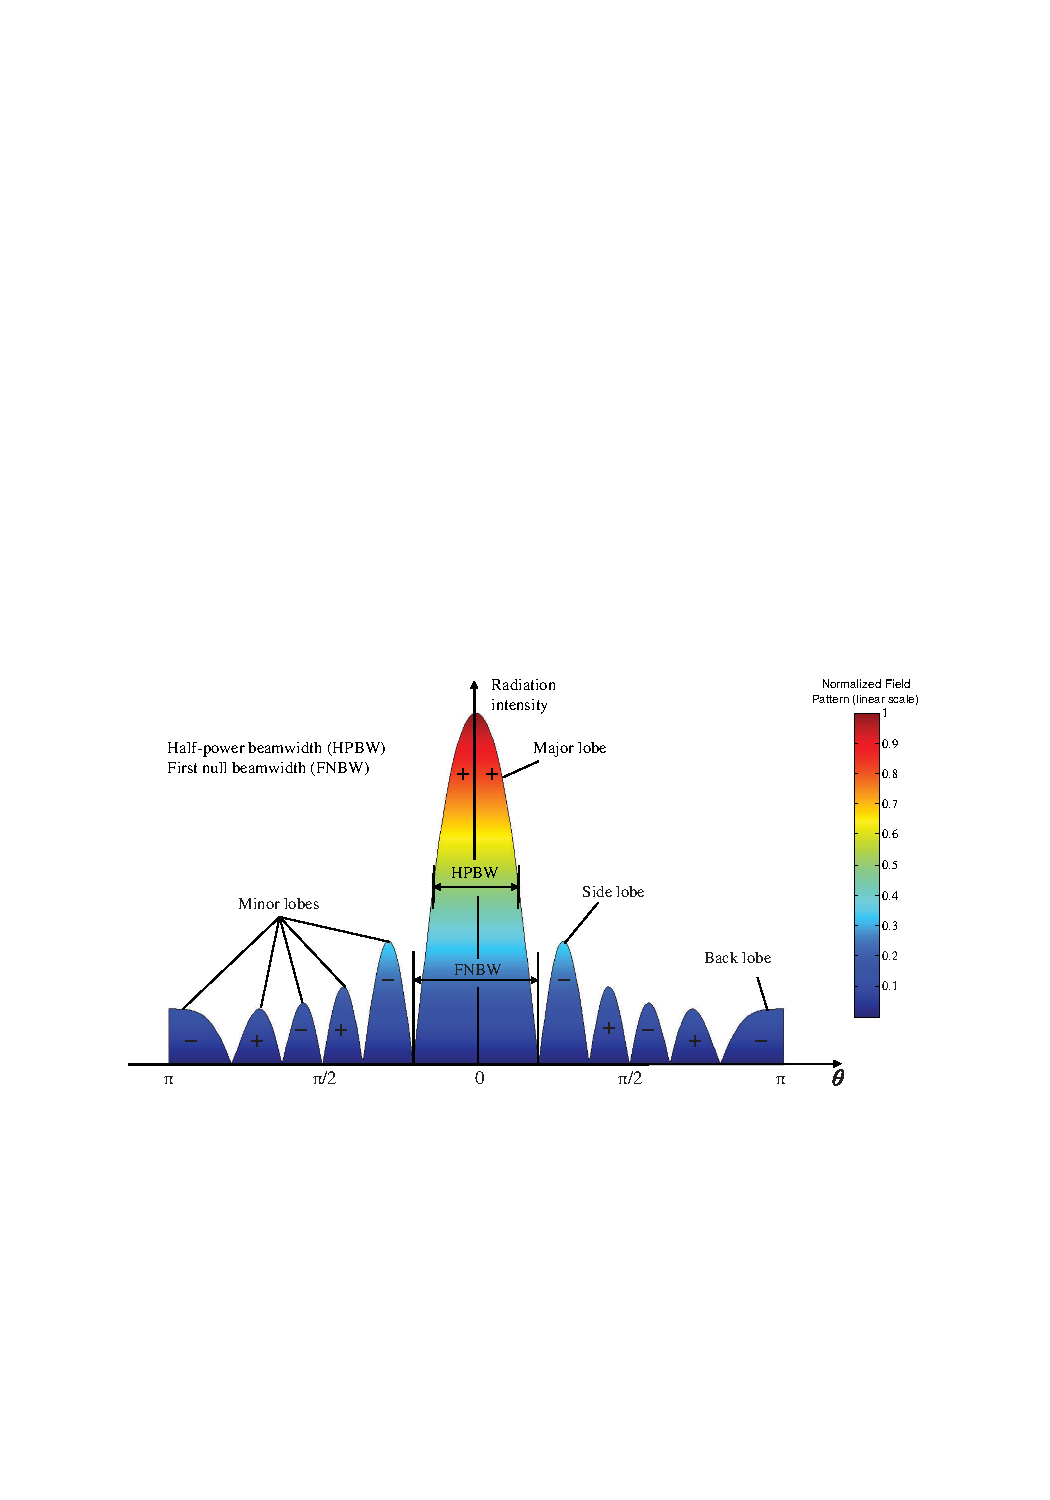
\includegraphics[width=14cm]{figure/5-2.pdf}
            \caption{\kaishu 某直角坐标下的功率方向图}\label{Fig: 天线方向图图例}
        \end{figure}

    \subsection{对称振子的辐射场}
        求解将对称振子分为许多小段,则每一小段都可看做一电基本振子,对于线性媒质,应用叠加原理,则对称振子的辐射场就等于这些无数小段基本振子辐射场的叠加。
        对称振子的电流分布近似为

        式中α:振子电流的相移常数。
        如果不考虑振子电流由辐射引起的
        衰减,忽略振子粗细的影响

    \subsection{辐射功率和辐射电阻}
        天线的输入功率一般为复功率,根据玻印廷定理,取包围天线所在体积$V$的任意封闭面$S$
        \begin{equation}
            \dot{p}_A=p_l+\dot{p}_\Sigma
        \end{equation}

        $V$内的损耗功率(导体损耗和介质损耗)
        \begin{equation}
            p_l=
        \end{equation}
        天线的全辐射功率
        =R+j2
        ='Reg,(E×H')-d.
        天线的辐射功率
        f
        辐射的无功功率
        =士1m)手,(E×H )-ask
        +j2o(Wm一WR)


        辐射功率与线天线上电流的大小有关,不便于直接比较天线的性能。为此引入天线的辐射阻抗概念。假设天线的全辐射功率被一个等效阻抗所“吸收”,该阻抗上流过的电流为天线上某处的电流,称此等效阻抗为天线的辐射阻抗。如天线上某处电流的振幅为I,则辐射阻抗
        \begin{equation}
            Z_\Sigma=\frac{P_\Sigma+\mathrm{j}Q_\Sigma}{\frac{1}{2}I^2}=R_\Sigma+\mathrm{j}X_\Sigma
        \end{equation}

        使用 波腹电流$I_M$ 或 输入电流$I_A$ 来计算,可以得到不同意义下的辐射阻抗$Z_\Sigma$和$Z_{\Sigma A}$,
        两种阻抗值不同,但满足
        
        \begin{equation}
            \frac{1}{2}=
        \end{equation}

        采用玻印廷矢量法计算天线的实辐射功率(以后简称辐射功率)和辐射电阻。

    \subsection{辐射功率和辐射阻抗}

        \begin{equation*}
        \mbox{计算辐射功率和辐射阻抗}
        \begin{cases}
            \mbox{远场区——Poynting矢量法,辐射实功率,辐射电阻}\\
            \mbox{近场区——感应电势法,复功率,辐射电阻和电抗}
        \end{cases}
        \end{equation*}

        远场区辐射功率
        \begin{equation}
            P_\Sigma=\frac{1}{120\pi}
        \end{equation}

        辐射电阻
        \begin{equation}
            R_\Sigma=\frac{2P_\Sigma}{|I_M|^2}=60 \int_{0}^{\pi}\frac{[]^2}{\sin\theta}\,\mathrm{d}\theta
        \end{equation}

    \subsection{天线的有效长度}
    \subsection{方向系数}
        天线的方向系数:用数字定量地表示辐射电磁能量集束程度,描述天线的方向特性数,又叫做方向性系数或方向性增益。
        
        
        \begin{definition}
        {辐射功率}
        {辐射功率}
            设有一球面$S$,半径为$r$,球心位于天线中心。天线的辐射功率,定义为\textbf{天线辐射场穿过球面$S$的功率}:
            \begin{equation}
                P_r(\vec{r})
                =\oint_S \vec{S}_r\cdot\mathrm{d}\vec{S}
            \end{equation}
        \end{definition}

        \begin{definition}
        {辐射强度}
        {辐射强度}
            天线在某方向的辐射强度,定义为\textbf{该方向上单位立体角内的辐射功率}:
            \begin{equation}
                U(\theta,\varphi)=
            \end{equation}
        \end{definition}

        \begin{definition}
        {方向系数}
        {方向系数}
            天线在某方向的方向系数$D(\theta,\varphi)$是该方向上的辐射强度$U(\theta,\varphi)$与平均辐射强度之比,平均辐射强度为$\frac{1}{4}$,即
            \begin{equation}
                D(\theta,\varphi)=\frac{4\pi F^2(\theta,\varphi)}{\int_{0}^{2\pi}\int_{0}^{\pi}F^2(\theta,\varphi)\sin\theta\,\mathrm{d}\theta\mathrm{d}\varphi}
            \end{equation}

            最大辐射方向的方向系数:某天线的方向系数通常均指最大辐射方向的方向系数。

        \end{definition}

        \begin{definition}
        {天线增益}
        {天线增益}
            天线的在某方向的增益$G(\theta,\varphi)$是该方向辐射强度$U(\theta,\varphi)$同天线 \underline{以同一输入功率} 向空间均匀辐射的辐射强度$\dfrac{P_A}{4\pi}$之比,即
            \begin{equation}
                G(\theta,\varphi)=4\pi \frac{U(\theta,\varphi)}{P_A}
            \end{equation}

            增益与方向系数的关系
            \begin{equation}
                G(\theta,\varphi)=D(\theta,\varphi)\eta_A
            \end{equation}

            某天线的增益通常指最大辐射方向增益:
            \begin{equation}
                G=4\pi \frac{U_M}{P_A}=D_M\eta_A
            \end{equation}
        \end{definition}

        
    \subsection{对称振子的输入阻抗}
    
\section{的}


% !TeX root = Microwave.tex
\chapter{缝隙天线和微带天线}

缝隙天线是在金属壁(同轴线、波导管、谐振器)上开窄缝($<\frac{1}{2}\lambda$)所形成的的天线。


    \paragraph{Lone等效原理}

\section{理想缝隙天线}

    \subsection{电磁场的巴俾涅原理和缝隙天线}
    
    \begin{theorem}{巴俾涅原理}{巴俾涅原理}
        巴俾涅原理用于论述互补平面屏(理想导电屏和理想导磁屏)的矢量电磁场问题。
    \end{theorem}

    \begin{corollary}{电屏和互补磁屏的互补原理}{电屏和互补磁屏的互补原理}
        ddd    
    \end{corollary}

    电屏(b)与互补电屏(d)之间的电磁场关系:
    \begin{subequations}
        \begin{numcases}{\mbox{}} 
            \vec{E}_e+Z_0 \vec{H}_d=\vec{E}^i\\
            \vec{H}_e-Y_0 \vec{E}_d=\vec{H}^i            
        \end{numcases}
    \end{subequations}


    无限大平板上的$\frac{\lambda}{2}$缝隙天线和半波振子具有互补的场分布。方向图相同,只是E面和H面互换。


    缝隙天线的辐射磁场:
    \begin{equation}
        \vec{E}_d=\mathrm{j}\frac{120U_M}{Z_0}\frac{\cos(kl\cos\theta)-\cos(kl)}{\sin\theta} \frac{\mathrm{e}^{-\mathrm{j}k r}}{r} \hat{\varphi}
    \end{equation}

    若令$U_M=0.5 Z_0I_M$,则它们的辐射场相同,因而辐射功率也相同。类比对称振子天线把辐射功率归于波腹电流和辐射电阻,缝隙天线的辐射功率可归于波腹电压和辐射电导:
    \begin{equation}
        P_{\varSigma '}=\frac{1}{2}\left\vert U_M\right\vert^2G_{\varSigma '}
    \end{equation}


\section{矩形波导缝隙天线}
    
    
    \subsection{波导缝隙天线阵列}
    为了增强天线阵列的方向性,在波导上按一定规律开出一系列尺寸相同的缝隙,构成波导缝隙阵列(Slot Array)。

    \paragraph{谐振式缝隙阵}
    \begin{enumerate}
    \renewcommand*\labelenumi{\circled{\theenumi}}
        \item 横向
        \item 纵向
    \end{enumerate} 

    \paragraph{非谐振式缝隙阵}
    若把谐振式缝隙阵的波导的末端改为匹配负载(使波导传输行波),且缝隙的间距不等于$\frac{\lambda}{2}$,则可以构成非谐振式缝隙阵。

    \underline{因为非谐振式缝隙阵是由行波激励的 ,所以能在较宽的频带内保持良好匹配,缺点是效率较低。}
    由天线阵列的理论,这种线性相位差的阵元构成的缝隙阵列,方向图指向与缝隙面法线的夹角为
    \begin{equation}
        \theta_M=\arcsin\left(\frac{\beta \lambda}{2 \pi d}\right)
    \end{equation}
    其中$\beta=\frac{2 \pi d}{\lambda_g}$。


    \paragraph{匹配偏斜缝隙阵}
    在窄壁上开斜缝,相邻斜缝之间的距离为$\frac{\lambda}{2}$,




    \subsection{波导缝隙阵的方向性}
    设$N$为缝隙个数,$\theta$为场点指向与缝隙平面法线的夹角。若各缝隙为等幅激励,则在$z$轴与缝隙平面法线所在的平面内:
    \begin{equation}
        f_a(\theta)=f(\theta)\frac{\sin\left[\frac{N}{2}(kd\sin\theta-\beta)\right]}{\sin\left[\frac{1}{2}(kd\sin\theta-\beta)\right]}
    \end{equation}



\section{微带天线}

    \subsection{微带天线的结构}

    \subsection{微带天线的辐射原理}

    \subsection{微带天线的分析方法}
    将矩形微带的两个开路端等效为两个缝隙天线。


\section{常见宽带天线}

    \subsection{菱形天线}    
    
    \subsection{螺旋天线}
        
    \subsection{非频变天线}
    任何天线,它的性能都是由电尺寸(长度与波长的比值,或者面积与波长的平方的比值)决定的。

    如果天线的所有尺寸和工作波长按同比例变化,则天线的辐射性质保持不变。

    \begin{enumerate}
    \renewcommand*\labelenumi{\circled{\theenumi}}
        \item 角度条件。 天线的几何形状只由角度角度决定,与其他尺寸无关。
        \item 终端效应弱。 天线向外辐射的功率主要在传输线上消耗。决定天线辐射特性的主要部分是载有较大电流的部分,而其延伸段的作用很小,在这种情况下,有限长天线具有与无限长天线相似的电性能。
    \end{enumerate}

    平面等角螺旋天线的结构和工作原理
    \begin{subequations}
        \begin{numcases}{\mbox{双臂四线的极坐标方程}} 
            r_1=r_0 \mathrm{e}^{\alpha \varphi}\\
            r_2=r_0 \mathrm{e}^{\alpha (\varphi-\delta)}\\
            r_3=r_0 \mathrm{e}^{\alpha (\varphi-\pi)}\\
            r_4=r_0 \mathrm{e}^{\alpha (\varphi-\pi-\delta)}
        \end{numcases}
    \end{subequations}

    自补结构是互补的特殊情况,互补天线的阻抗有如下性质:
    % \begin{equation}
    %     Z_\mbox{缝隙}Z_\mbox{天线}
    % \end{equation}

    \begin{itemize}
        \item 当频率很低时,全臂长比波长小得多时,为线极化(近似看作对称振子);
        \item 当频率增大时,最终形成圆极化,极化旋向和螺旋绕向有关。在许多实用情况下,轴比小于等于2的典型值发生在全臂长约为一个波长时。
    \end{itemize}


    阿基米德螺旋天线

    \begin{subequations}
        \begin{numcases}{\mbox{双臂双线}} 
            r_1=r_0 \varphi\\
            r_1=r_0 (\varphi-\pi)
        \end{numcases}
    \end{subequations}


    对数周期天线。天线的齿形结构按一定比例发生变化。

    对数周期偶极子天线(LPDA)
    \begin{equation}
        \tau=\frac{l_n}{l_{n-1}}=\frac{R_n}{R_{n-1}}=\frac{d_n}{d_{n-1}}
    \end{equation}

    因此
    \begin{equation}
        \ln f_n -\ln f_{n-1} =\ln \tau
    \end{equation}
    它的非频变特性频率连续变化时,电性能周期性变化。


    
    \subsection{引向天线}

    引向天线,又称为八木天线或波道天线。广泛应用于米波和分米波通信、雷达、电视。

    反射振子和引向振子都是短路无源振子,无源振子的中心固定在与他们垂直的金属杆上,有源振子则与金属杆绝缘。有源振子通常为半波谐振长度。

    作为反射器时,无源短路振子上的电流相位超前于有源振子;作为引向器时,电流相位滞后。可以通过调节其长度改变感应电流的相位差,也可以改变到无源振子的距离改变耦合电流的相位差。

    调节反反射振子和引向振子的长度以及相邻振子间距,使各振子电流相位自反射振子到最后一个引向振子依次滞后,从而实现天线在前向从有源振子到引向振子的方向发生在最大辐射方向

    对于$N$元引向天线,第1个振子为反射振子,第2振子为有源振子,第3到第$N$振子为引向振子,则
    阵因子取决于各单元间距和电流比
    \begin{equation}
        f_a(\theta,\varphi)=\left\vert \sum_{i=1}^{N}\left\vert \frac{I_{M1}}{I_{Mi}}\right\vert \mathrm{e}^{\mathrm{j}\varPhi_i}\right\vert\;,\quad \varPhi_i=(\beta_i-\beta)+kd\sin\theta\cos \varphi
    \end{equation}



\section{面天线}

    天线阵虽然可获得很高的方向增益,但存在馈电复杂,功率容量低等缺点。

    面天线的组成:
    \begin{itemize}
        \item 初级源:如抛物面天线的喇叭馈源
        \item 形成方向性的部件:如抛物面反射器
    \end{itemize}

    \subsection{面天线的基本理论和分析方法}

    面天线的基本问题是确定它的辐射场

    在麦克斯韦方程组中引入等效磁荷和等效磁流,使方程组形式对称。

    在距离无限远处,电磁场
    \begin{subequations}
        \begin{numcases}{\mbox{}} 
            E=B_0\frac{\mathrm{e}^{-\mathrm{j}kr}}{r}\hat{e}_0\\
            H=\frac{\mu}{\varepsilon}
        \end{numcases}
    \end{subequations}

    \paragraph{辅助源法}

    所谓辅助源,首先引入洛伦兹辅助定理。设辅助电流源$J_1^e$,辅助磁流元$J_1^m$


    \subsection{等效原理}

    某一区域内产生的电磁场可由

    \begin{subequations}
        \begin{numcases}{\mbox{}} 
            \vec{J}_1^e=\hat{n}\times \vec{H}\\
            \vec{J}_1^m=-\hat{n}\times \vec{E}
        \end{numcases}
    \end{subequations}


    克希霍夫公式
    \begin{equation}
        \vec{E}_p=
    \end{equation}

    面天线采用\underline{方向系数},\underline{增益},\underline{口径利用效率},\underline{有效面积}和\underline{噪声温度}等参数描述其电性能。

    \begin{enumerate}
    \renewcommand*\labelenumi{(\theenumi)}
        \item 方向系数
        
        这里主要讨论相同场平面口径天线

        \begin{equation}
            D=\frac{4 \pi}{\lambda^2}A_e=\frac{4 \pi}{\lambda^2}A\eta
        \end{equation}
        \item 口径利用效率
    \end{enumerate}


    \subsection{平面口径的绕射问题}


%%%%%%
\begin{appendices}
    % !TeX root = Microwave.tex
\chapter{引用}
\section{省略的证明过程}
\begin{enumerate}
    \renewcommand*\labelenumi{\circled{\theenumi}}
    \item 函数是从数到数的映射。
    \item 泛函是从函数到数的映射。
    \item 算子是从函数到函数的映射。
\end{enumerate}
\section{坐标系}
    \subsection{广义正交坐标系}
    
    与直角坐标系不同,正交曲线坐标系的单位基向量$\hat{e}_i$通常不是常矢量。它们模始终为1,但方向可能随空间中一点位置不同而变化。

    \begin{definition}{正交曲线坐标系}{正交曲线坐标系}
        三个有序数$(u_1,u_2,u_3)$,满足
        \begin{enumerate}
            \renewcommand*\labelenumi{(\theenumi)}
            \item $u_i=u_i(x,y,z)$是直角坐标$(x,y,z)$的单值函数;
            \item $\hat{e}_1,\hat{e}_2,\hat{e}_3$是曲线$u_1,u_2,u_3$的切线上指向$u_1,u_2,u_3$增大一方的单位矢量,它们两两正交,且满足右手螺旋关系:
            \begin{equation*}
                \hat{e}_1\times \hat{e}_2=\hat{e}_3\,,\;
                \hat{e}_2\times \hat{e}_3=\hat{e}_1\,,\;
                \hat{e}_3\times \hat{e}_1=\hat{e}_2
            \end{equation*}
        \end{enumerate}
        则称$(u_1,u_2,u_3)$构成的坐标系为正交曲线坐标系。
    \end{definition}



    正交坐标系使用曲线坐标$(u_1,u_2,u_3)$,局部单位基向量为$\hat{e}_1,\hat{e}_2,\hat{e}_3$,$h_i,\,i=1,2,3$为对应的拉梅(\emph{Lame})系数。$\varPhi$为标量,矢量$\vec{A}=(A_1,A_2,A_3)$则:
    \begin{subequations}
        \begin{align}
            \nabla \varPhi&=\frac{1}{h_1}\frac{\partial \varPhi}{\partial u_1}\hat{e}_1+\frac{1}{h_2}\frac{\partial \varPhi}{\partial u_2}\hat{e}_2+\frac{1}{h_3}\frac{\partial \varPhi}{\partial u_3}\hat{e}_3\\
            \nabla\cdot\vec{A}&=\frac{1}{h_1h_2h_3}\left[\frac{\partial }{\partial u_1}(h_2h_3A_1)+\frac{\partial }{\partial u_2}(h_1h_3A_2)+\frac{\partial }{\partial u_3}(h_1h_2A_3)\right]\\
            \nabla\times\vec{A}&=\frac{1}{h_1h_2h_3}\begin{vmatrix}
            h_1\hat{e}_1&h_2\hat{e}_2&h_3 \hat{e}_3\\
            \frac{\partial }{\partial u_1}&\frac{\partial }{\partial u_2}&\frac{\partial }{\partial u_3}\\
            h_1A_1&h_2A_2&h_3 A_3
        \end{vmatrix}
        \end{align}
    \end{subequations}

    \subsection{\emph{Lame}系数}
    \paragraph{如何求拉梅系数?}
    “拉梅系数是坐标曲线的一组特殊切向量的模。”
    \begin{equation}
        h_i=|\bm{h}_i|
    \end{equation}
    其中
    \begin{equation}
        \bm{h}_i=\frac{\partial \bm{x}}{\partial u_i}=\left(\frac{\partial x_1}{\partial u_i},\frac{\partial x_2}{\partial u_i},\frac{\partial x_3}{\partial u_i}\right),\;i=1,2,3
    \end{equation}
    只有当切向量$\bm{h}_1,\bm{h}_2,\bm{h}_3$两两正交时,曲线坐标系是曲线正交坐标系,才有拉梅系数定义。
    其中$\bm{x}=(x_1,x_2.x_3)$为空间中一点的笛卡尔坐标系描述,$(u_1,u_2,u_3)$为该曲线坐标系对该点的描述。\\
    这里只考虑了3维的情况:涉及拉梅系数,就一定涉及到一个特定3维空间的广义正交坐标系表示和笛卡尔坐标系表示之间的关系。

    例如:
    \begin{equation}
        \mbox{柱坐标系}\left\{\begin{aligned}
            &\bm{h}_1=\left(\frac{\partial \cos\phi}{\partial \rho},\frac{\partial \sin\phi}{\partial \rho},\frac{\partial z}{\partial \rho}\right)\\
            &\bm{h}_2=\left(\frac{\partial \cos\phi}{\partial \phi},\frac{\partial \sin\phi}{\partial \phi},\frac{\partial z}{\partial \phi}\right)\\
            &\bm{h}_3=\left(\frac{\partial \cos\phi}{\partial z},\frac{\partial \sin\phi}{\partial z},\frac{\partial z}{\partial z}\right)
        \end{aligned}\right.
        \Rightarrow
        \left\{\begin{aligned}
            &h_1=|\left(\cos\phi,\sin\phi,0\right)|=1\\
            &h_2=|\left(-\rho\sin\phi,\rho\cos\phi,0\right)|=\rho\\
            &h_3=|\left(0,0,1\right)|=1
        \end{aligned}\right.
    \end{equation}
    \begin{equation}
        \begin{aligned}
            \mbox{球坐标系}\left\{\begin{aligned}
                &\bm{h}_1=\left(\frac{\partial r\sin\theta\cos\phi}{\partial r},\frac{\partial r\sin\theta\sin\phi}{\partial r},\frac{\partial r\cos\theta}{\partial r}\right)\\
                &\bm{h}_2=\left(\frac{\partial r\sin\theta\cos\phi}{\partial \theta},\frac{\partial r\sin\theta\sin\phi}{\partial \theta},\frac{\partial r\cos\theta}{\partial \theta}\right)\\
                &\bm{h}_3=\left(\frac{\partial r\sin\theta\cos\phi}{\partial \phi},\frac{\partial r\sin\theta\sin\phi}{\partial \phi},\frac{\partial r\cos\theta}{\partial \phi}\right)
            \end{aligned}\right.\\
            \Rightarrow
            \left\{\begin{aligned}
                &h_1=|\left(\sin\theta\cos\phi,\sin\theta\sin\phi,\cos\theta\right)|=1\\
                &h_2=|\left(r\cos\theta\cos\phi,r\cos\theta\cos\phi,-r\sin\theta\right)|=r\\
                &h_3=|\left(-r\sin\theta\sin\phi,r\sin\theta\cos\phi,0\right)|=r\sin\theta
            \end{aligned}\right.
        \end{aligned}
    \end{equation}
\section{公式与定理}
    \subsection{华里士公式}
    \begin{equation}
        \int_{0}^{\frac{\pi}{2}}\sin^nx\,\mathrm{d}x=
        \left\{
            \begin{aligned}
                &\frac{n-1}{n}\cdot\frac{n-3}{n-2}\cdot\,\cdots\,\cdot\frac{3}{4}\cdot\frac{1}{2}{\,\color{red}\cdot\,\frac{\pi}{2}}\;,\quad \mathrm{even} ~n\\
                &\frac{n-1}{n}\cdot\frac{n-3}{n-2}\cdot\,\cdots\,\cdot\frac{4}{5}\cdot\frac{2}{3}\;,\quad \mathrm{odd} ~n
            \end{aligned}
        \right.
    \end{equation}

    \subsection{矢量恒等式}
    \begin{subequations}
        \begin{align}
            &\nabla\cdot(\nabla\times\vec{A})=0&\mbox{“旋无源”}\\
            &\nabla\times(\nabla \varphi)=\vec{0}&\mbox{“梯无旋”}\\
            &\nabla\times \nabla\times\vec{A}=\nabla(\nabla\cdot\vec{A})-\nabla^2 \vec{A}&
        \end{align}
    \end{subequations}

    \subsection{斯托克斯公式}
    设矢量$\vec{A}\in \mathbb{R}^3$的三个分量都在有向曲面$S$及其边界$\partial S=\Gamma$上具有连续的一阶偏导数,且$\Gamma$的正向与$S$的侧符合右手规则,则:
    \begin{equation}
        \iint_S \nabla\times\vec{A}\cdot\mathrm{d}\vec{S}
        =\oint_\Gamma \vec{A}\cdot\mathrm{d}\vec{r}
    \end{equation}

    % !TeX root = Microwave.tex
\chapter{习题}
\section{作业2-3}
\begin{center}
    姓名:韩玉千\hspace{4cm}学号:19020100423
\end{center}

    \paragraph{1}矩形波导$a\times b=22.86\times 10.16\,\si{\square\milli\metre}$,求主模 TE{\scriptsize 10}模的可能工作频率范围。
    \\{\bfseries 解:}\\
    根据 TE{\scriptsize 10}模的截止特性:
    \begin{equation*}
        \beta^2=k^2-k_c^2=(\frac{2\pi}{\lambda})^2-(\frac{\pi}{a})^2>0
    \end{equation*}
    因此
    \begin{equation}
        \lambda<2a\label{Equ: Cut-off Characteristics of TE10}
    \end{equation}
    矩形波导在传输主模时,要求第二模TE{\scriptsize 20}模为凋落模。因此有单模传输条件:
    \begin{equation}
        \lambda>\lambda_{c20}=\frac{2}{\sqrt{(\frac{2}{a})^2+(\frac{0}{b})^2}}=a\label{Equ: Sigle Mode Condition}
    \end{equation}
    结合式(\ref{Equ: Cut-off Characteristics of TE10})和(\ref{Equ: Sigle Mode Condition}),则波长应满足:
    \begin{equation*}
        \lambda\in(a,2a)
    \end{equation*}
    对应工作频率:
    \begin{equation*}
        f\in\left(\frac{c}{2a},\frac{c}{a}\right)
    \end{equation*}
    \rightline{where $c=\SI{3e8}{\metre\per\second}\qquad$}
    得
    \begin{equation*}
        \SI{6.56}{\giga\hertz} < f < \SI{13.12}{\giga\hertz}
    \end{equation*}

    \paragraph{2}画出 TE{\scriptsize 10}模电磁场$E_y, H_x, H_z$的具体场型图。
    \\{\bfseries 解:}如图\ref{Fig: 2-3(2)}所示。\\
    \begin{figure}[htp]
        \centering
        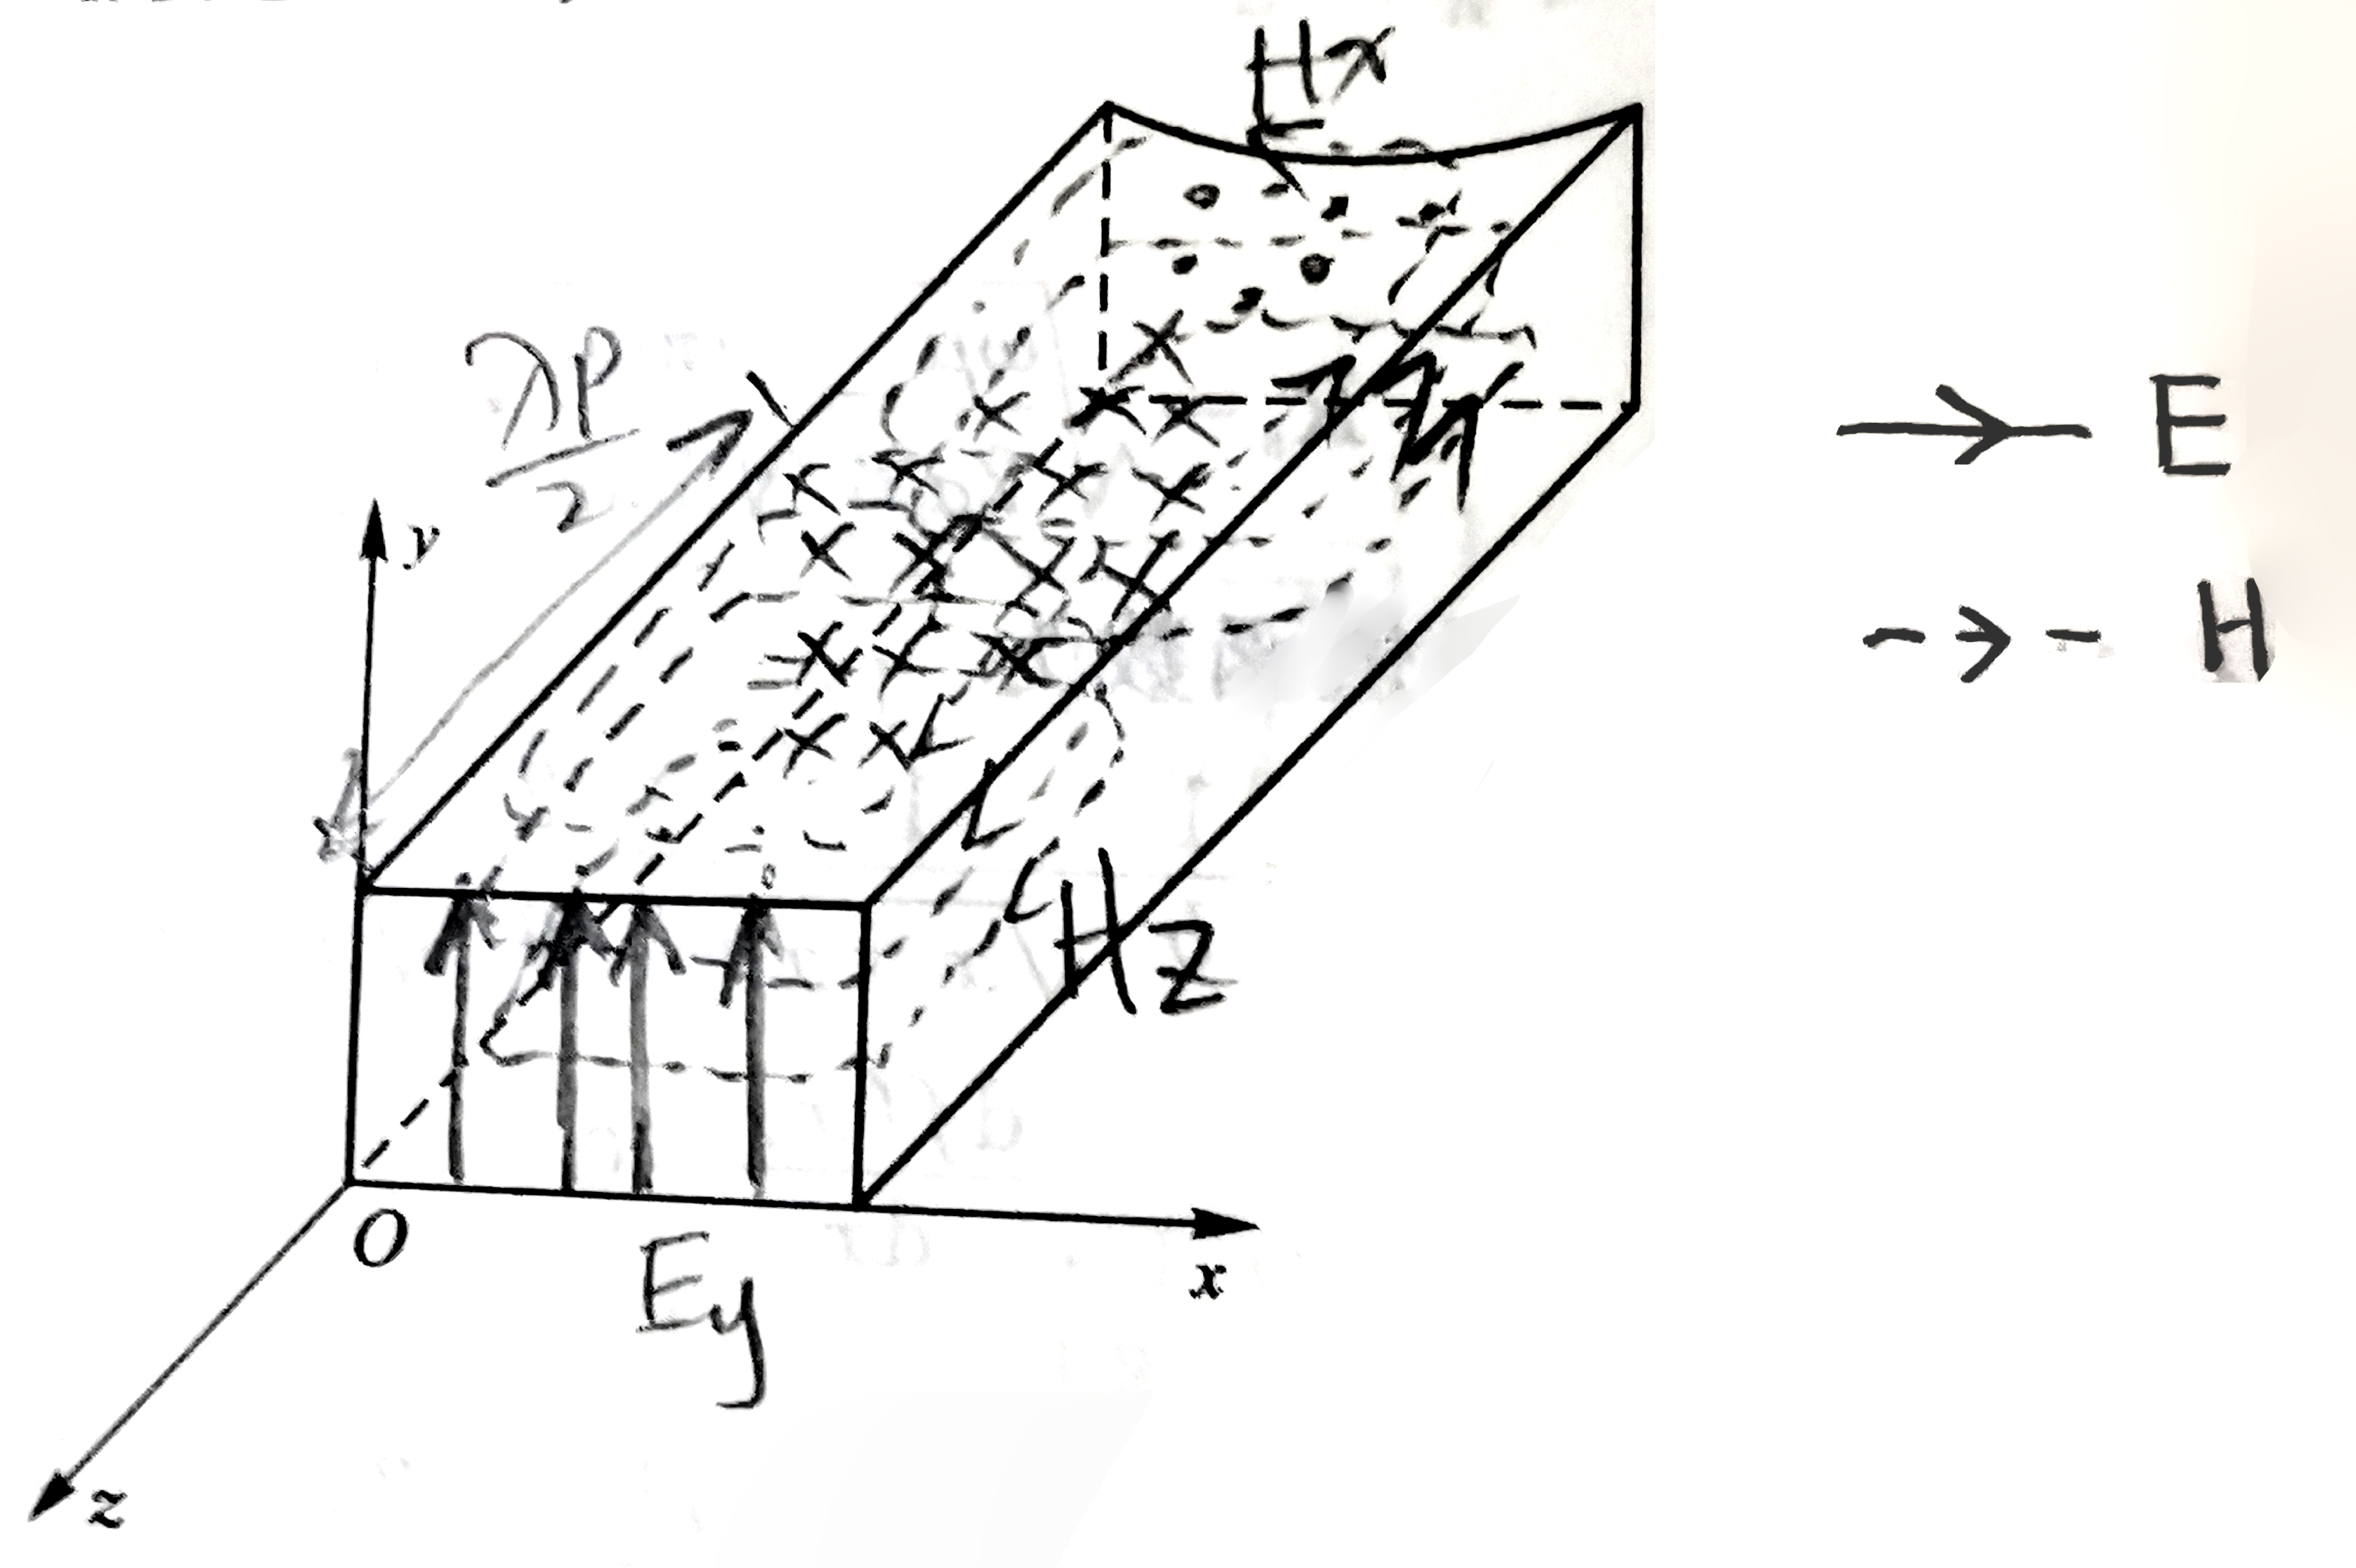
\includegraphics[width=10cm]{figure/appendix/2-3(2).jpg}
        \caption{\kaishu 2-3第二题图}\label{Fig: 2-3(2)}
    \end{figure}
    \paragraph{3}画出宽壁$y=0$的表面电流分布。指出何处$J_z$最大。
    \\{\bfseries 解:}如图\ref{Fig: 2-3(3)}所示。\\
    对于 TE{\scriptsize 10}模,宽壁内表面切向的磁场分量$H_s=H_x$,因此:
    \begin{equation*}
        J_z=\left[\hat{n}\times H_s\right]_{y=0}=\left[\hat{y}\times H_x\right]_{y=0}=-H_x|_{y=0}=\frac{\beta a}{\pi}H_0\sin\left(\frac{\pi}{a}x\right)\sin(\omega t-\beta z)
    \end{equation*}
    因此在$x=\frac{a}{2}$处取得最大值
    \begin{figure}[htp]
        \centering
        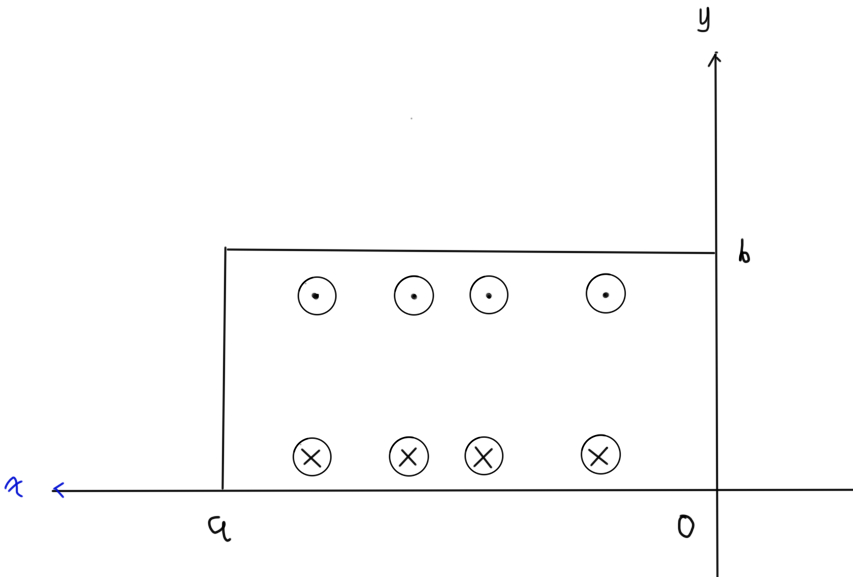
\includegraphics[width=8cm]{figure/appendix/2-3(3).jpg}
        \caption{\kaishu 2-3第三题图}\label{Fig: 2-3(3)}
    \end{figure}

\section{作业2-4}
    \paragraph{1}已知矩形波导如图\ref{Fig: 2-4(1)}所示,分别写出 TE{\scriptsize 11}模和 TM{\scriptsize 11}模的一般场方程。若要求它们是凋落模,写出条件。
    \begin{figure}[htp]
        \centering
        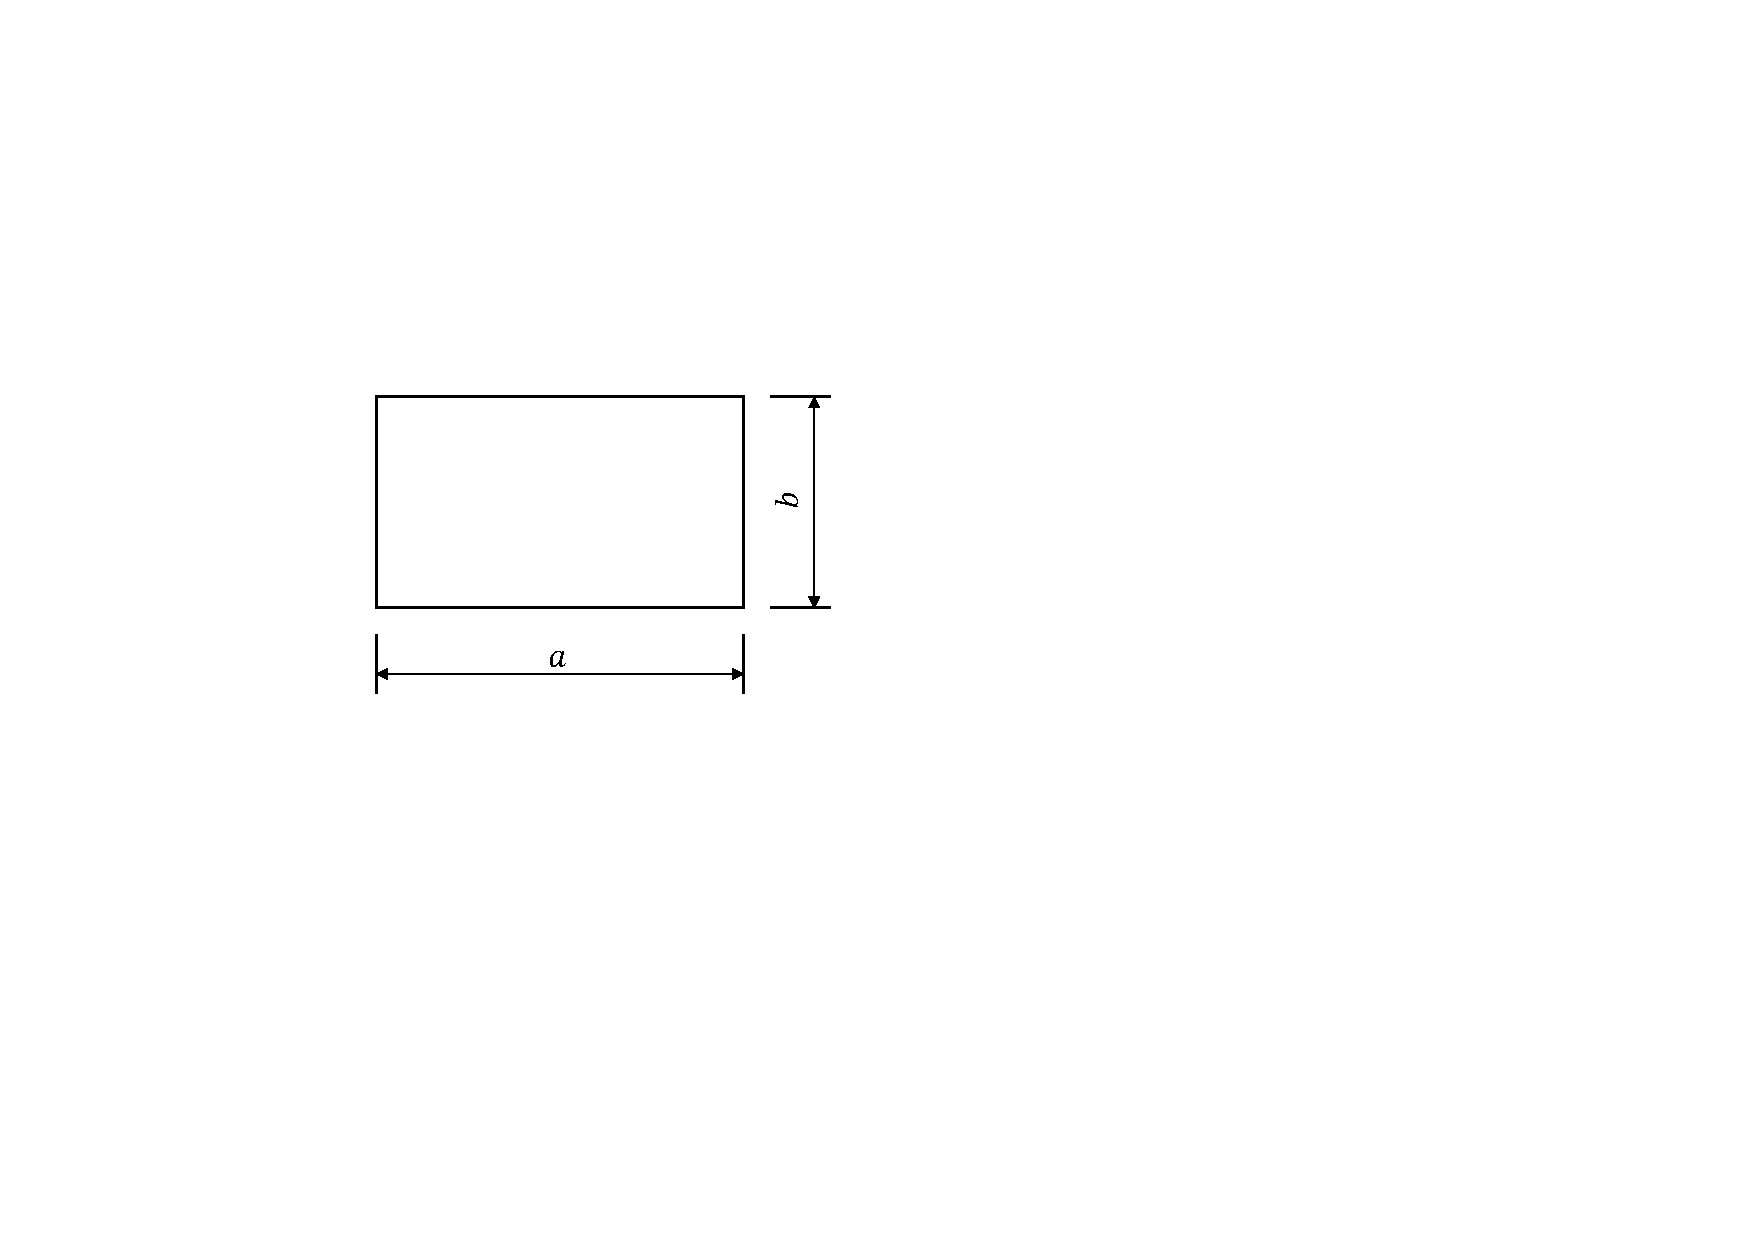
\includegraphics[width=6cm]{figure/appendix/2-4(1).pdf}
        \caption{\kaishu 2-4第一题图}\label{Fig: 2-4(1)}
    \end{figure}
    \\{\bfseries 解:}\\
    对于 TE{\scriptsize 11}模:
    \begin{subequations}
        \begin{numcases}{\mbox{TE{\scriptsize 11}纵向场}}
            E_z=0 \\
            H_z=H_0\cos{\left(\frac{\pi}{a}x\right)}\cos{\left(\frac{\pi}{b}y\right)}\mathrm{e}^{-\gamma z}
        \end{numcases}
    \end{subequations}
    其中$\gamma$满足$\gamma^2=k_c^2-k^2$,$k^2=\omega^2\mu \varepsilon$,$H_0$由激励决定。


    由纵向分量法,
    \begin{equation}
        \begin{bmatrix}
            E_x\\E_y\\H_x\\H_y
        \end{bmatrix}
        =\frac{1}{k_c^2}\begin{bmatrix}
            -\gamma&0&0&-\mathrm{j}\omega \mu\\
            0&-\gamma&\mathrm{j}\omega \mu&0\\
            0&\mathrm{j}\omega \varepsilon&-\gamma&0\\
            -\mathrm{j}\omega \varepsilon&0&0&-\gamma\\
        \end{bmatrix}
        \begin{bmatrix}
            \frac{\partial E_z}{\partial x}\\\frac{\partial E_z}{\partial y}\\\frac{\partial H_z}{\partial x}\\\frac{\partial H_z}{\partial y}
        \end{bmatrix}
    \end{equation}
    得:
    \begin{subequations}
        \begin{numcases}{\mbox{TE{\scriptsize 11}横向场}}
            E_x=\mathrm{j}\frac{\omega \mu}{k_c^2}\left(\frac{\pi}{b}\right)H_0\cos{\left(\frac{\pi}{a}x\right)}\sin{\left(\frac{\pi}{b}y\right)}\mathrm{e}^{-\gamma z}\\
            E_y=-\mathrm{j}\frac{\omega \mu}{k_c^2}\left(\frac{\pi}{a}\right)H_0\sin{\left(\frac{\pi}{a}x\right)}\cos{\left(\frac{\pi}{b}y\right)}\mathrm{e}^{-\gamma z}\\
            H_x=\frac{\gamma}{k_c^2}\left(\frac{\pi}{a}\right)H_0\sin{\left(\frac{\pi}{a}x\right)}\cos{\left(\frac{\pi}{b}y\right)}\mathrm{e}^{-\gamma z}\\
            H_y=\frac{\gamma}{k_c^2}\left(\frac{\pi}{b}\right)H_0\cos{\left(\frac{\pi}{a}x\right)}\sin{\left(\frac{\pi}{b}y\right)}\mathrm{e}^{-\gamma z}
        \end{numcases}
    \end{subequations}
    对于 TM{\scriptsize 11}模,将$E_z$分离变量$E_z=X(x)Y(y)$代入$\frac{\nabla^2_tE_z}{E_z}+k_c^2=0$,得
    \begin{equation}
        E_z=E_0\cos(k_xx+\varphi_x)\cos(k_yy+\varphi_y)\mathrm{e}^{-\gamma z}
    \end{equation}
    由纵向场法,
    \begin{subequations}
        \begin{numcases}{}
            E_x=E_0\frac{\gamma}{k_c^2}k_x\sin(k_xx+\varphi_x)\cos(k_yy+\varphi_y)\mathrm{e}^{-\gamma z} \\
            E_y=E_0\frac{\gamma}{k_c^2}k_y\cos(k_xx+\varphi_x)\sin(k_yy+\varphi_y)\mathrm{e}^{-\gamma z}
        \end{numcases}
    \end{subequations}
    将其代入矩形波导的边界条件
    \begin{subequations}
        \begin{numcases}{}
            E_y|_{x=0,a}=0 \\
            E_x|_{y=0,b}=0
        \end{numcases}
    \end{subequations}
    解得:
    \begin{subequations}
        \begin{numcases}{}
            k_x=\frac{m\pi}{x}\\
            k_y=\frac{n\pi}{b}\\
            \varphi_x=\frac{\pi}{2}\\
            \varphi_y=\frac{\pi}{2}
        \end{numcases}
    \end{subequations}
    其中$m=1,n=1$。因此得:
    \begin{subequations}
        \begin{numcases}{\mbox{TM{\scriptsize 11}纵向场}}
            E_z=E_0\sin{\left(\frac{\pi}{a}x\right)}\sin{\left(\frac{\pi}{b}y\right)}\mathrm{e}^{-\gamma z} \\
            H_z=0
        \end{numcases}
    \end{subequations}
    其中$\gamma$满足$\gamma^2=k_c^2-k^2$,$k^2=\omega^2\mu \varepsilon$,$E_0$由激励决定。


    同理由纵向场法,可以表示横向场:
    \begin{subequations}
        \begin{numcases}{\mbox{TM{\scriptsize 11}横向场}}
            E_x=-\frac{\gamma}{k_c^2}\left(\frac{\pi}{a}\right)E_0\cos{\left(\frac{\pi}{a}x\right)}\sin{\left(\frac{\pi}{b}y\right)}\mathrm{e}^{-\gamma z}\\
            E_y=-\frac{\gamma}{k_c^2}\left(\frac{\pi}{b}\right)E_0\sin{\left(\frac{\pi}{a}x\right)}\cos{\left(\frac{\pi}{b}y\right)}\mathrm{e}^{-\gamma z}\\
            H_x=\mathrm{j}\frac{\omega \varepsilon}{k_c^2}\left(\frac{\pi}{b}\right)E_0\sin{\left(\frac{\pi}{a}x\right)}\cos{\left(\frac{\pi}{b}y\right)}\mathrm{e}^{-\gamma z}\\
            H_y=-\mathrm{j}\frac{\omega \varepsilon}{k_c^2}\left(\frac{\pi}{a}\right)E_0\cos{\left(\frac{\pi}{a}x\right)}\sin{\left(\frac{\pi}{b}y\right)}\mathrm{e}^{-\gamma z}
        \end{numcases}
    \end{subequations}

    TE{\scriptsize 11}模和 TM{\scriptsize 11}模,其截止波长为
    \begin{equation*}
        \lambda_c=\frac{2}{\sqrt{\left(\frac{1}{a}\right)^2+\left(\frac{1}{b}\right)^2}}=\frac{2ab}{\sqrt{a^2+b^2}}
    \end{equation*}
    因此,当$\lambda>\frac{2ab}{\sqrt{a^2+b^2}}$时,TE{\scriptsize 11}模和 TM{\scriptsize 11}模为凋落模。
    \\[15pt]
    \paragraph{2}BJ-48波导工作在\SI{5}{\centi\metre}波段。$f\in[3.94\sim5.99]\si{\giga\hertz}$,$a\times b=47.55\times 22.15\,\si{\square\milli\metre}$,检验其是否符合波导设计标准。
    \\{\bfseries 解:}\\
    \begin{equation*}
        \lambda\in\left(\frac{c}{f_{max}},\frac{c}{f_{min}}\right)=\left(\SI{50.0835}{\milli\metre},\SI{76.1421}{\milli\metre}\right)
    \end{equation*}
    符合标准的波导参数$\hat{a},\hat{b}$,应满足:
    \begin{subequations}
        \begin{numcases}{}
            \mbox{功率容量尽量大:}\hat{a}>0.555 \lambda\\
            \mbox{TE{\scriptsize 10}传输条件:}2\hat{a}>\lambda\\
            \mbox{TE{\scriptsize 20}截止条件:}\hat{a}<\lambda\\
            \mbox{加宽频带}\frac{\hat{b}}{\hat{a}}<0.5
        \end{numcases}
    \end{subequations}
    因此:
    \begin{subequations}
        \begin{numcases}{}
            \hat{a}>0.555 \lambda_{max}=\SI{42.2589}{\milli\metre} \\
            \hat{a}<\lambda_{min}=\SI{50.0835}{\milli\metre}
        \end{numcases}
    \end{subequations}
    因此参数a满足条件。又
    \begin{equation*}
        \frac{b}{a}=\frac{22.15}{47.55}=0.4658<0.5
    \end{equation*}
    因此参数b也满足条件。

\section{作业2-6}
\begin{center}
\end{center}

    \paragraph{1}空气填充的圆波导内传输 TE{\scriptsize 01}模,已知$\frac{\lambda}{\lambda_c}=0.9$,$f=\SI{5}{\giga\hertz}$,求$\lambda_g$和$\beta$。若波导半径扩大一倍,$\beta$有何变化?
    \\{\bfseries 解:}\\
    TE{\scriptsize 01}模是圆波导中损耗最小的模,其截止波长为:
    \begin{equation*}
        \lambda_c=1.641R
    \end{equation*}
    电磁波波长
    \begin{equation*}
        \lambda=\frac{c}{f}=\frac{\SI{3e8}{\metre}}{\SI{5}{\giga\hertz}}=\SI{60}{\milli\metre}
    \end{equation*}
    因此,导波波长
    \begin{equation*}
        \lambda_g =\frac{\lambda}{\sqrt{1-\left(\frac{\lambda}{\lambda_c}\right)^2}}=\SI{137.65}{\milli\metre}
    \end{equation*}
    同时解得
    \begin{equation*}
        R=\frac{\lambda}{0.9\times 1.641}=\SI{40.63}{\milli\metre}
    \end{equation*}
    \begin{equation*}
        \beta=\frac{2\pi}{\lambda_g}=\SI{45.64}{\radian\per\metre}
    \end{equation*}
    当波导的半径扩大一倍,$\lambda_c$增大一倍,$\lambda_g $减小,$\beta$增大。
    \\[15pt]
    \paragraph{2}对工作频率为\SI{3}{\giga\hertz}的发射机,用矩形波导和圆波导馈电,均用主传输模,试比较尺寸的大小。
    \begin{equation*}
        \lambda=\frac{c}{f}=\frac{\SI{3e8}{\metre\per\second}}{\SI{3}{\giga\hertz}}=\SI{100}{\milli\metre}
    \end{equation*}
        传输 TE{\scriptsize 10}的矩形波导,有
        \begin{subequations}
            \begin{numcases}{}
                0.555 \lambda<a<\lambda \\
                \frac{\hat{b}}{a}<0.5
            \end{numcases}
        \end{subequations}
        因此$a_{max}=\lambda$,对应$b_{max}=0.5\lambda$。


        传输 TE{\scriptsize 11}模的圆形波导,有
        \begin{equation}
            \lambda_{c TM_{01}}<\lambda<\lambda_{c TE_{11}}
        \end{equation}
        即
        \begin{equation*}
            2.62R<\lambda<3.412R
        \end{equation*}
        因此
        \begin{equation*}
            R\in\left(\frac{\lambda}{3.412},\frac{\lambda}{2.62}\right)
        \end{equation*}
        综上,矩形波导尺寸最大为$ab=0.5 \lambda^2$,圆波导尺寸最大为$\pi R^2=\frac{\pi}{2.62^2}\lambda^2=0.4577\lambda^2$。
    \\[15pt]
    \paragraph{3}已知半径为R的圆波导,电场有唯一分量
    \begin{equation*}
        E_\phi=E_0 \mathrm{J}_1\left(\frac{3.832}{R}r\right)\mathrm{e}^{-\mathrm{j}\beta z}
    \end{equation*}
    \begin{enumerate}
        \renewcommand*\labelenumi{(\theenumi)} %设置enumerate标号为一对圆括号
        \item 它是TE还是TM模式?
        \item 求磁场$\vec{H}$;
        \item 分析它的模式指数$m,n$并说出其物理意义;
        \item 画出场型图。
    \end{enumerate}
    ~\\{\bfseries 解:}\\
    (1):由于电场没有纵向分量,因此为TE模式。\\
    (2):$\vec{H}=\frac{1}{-\mathrm{j}\omega\mu}\nabla\times\vec{E}$,在柱坐标系下:
    \begin{align}
        \vec{H}&=\frac{1}{-\mathrm{j}\omega\mu}\cdot\frac{1}{r}\begin{vmatrix}
            \hat{r}&r\hat{\phi}&\hat{z}\\
            \frac{\partial }{\partial r}&\frac{\partial }{\partial \phi}&\frac{\partial }{\partial z}\\
            E_r&rE_\phi&E_z
        \end{vmatrix}\\
        &=\frac{1}{-\mathrm{j}\omega\mu}\cdot\frac{1}{r}\begin{vmatrix}
            \hat{r}&r\hat{\phi}&\hat{z}\\
            \frac{\partial }{\partial r}&\frac{\partial }{\partial \phi}&\frac{\partial }{\partial z}\\
            0&rE_0 \mathrm{J}_1\left(\frac{3.832}{R}r\right)\mathrm{e}^{-\mathrm{j}\beta z}&0
        \end{vmatrix}\notag\\
        &=\frac{\mathrm{j}}{\omega\mu r}\left[\hat{r}\mathrm{j}\beta rE_0 \mathrm{J}_1\left(\frac{3.832}{R}r\right)\mathrm{e}^{-\mathrm{j}\beta z}+\hat{z}E_0 \mathrm{e}^{-\mathrm{j}\beta z}\frac{\partial r\mathrm{J}_1\left(\frac{3.832}{R}r\right)}{\partial r}\right]\notag
    \end{align}
    根据递推公式
    \begin{equation}
        x \mathrm{J}_m'\left(x\right)+m \mathrm{J}_m\left(x\right)=x \mathrm{J}_{m-1}\left(x\right)
    \end{equation}
    有
    \begin{equation}
        \frac{\mathrm{d}}{\mathrm{d}x} \left[x \mathrm{J}_1\left(x\right)\right]=x\mathrm{J}_0\left(x\right)
    \end{equation}
    因此,$\frac{\partial r\mathrm{J}_1\left(\frac{3.832}{R}r\right)}{\partial r}=\frac{\partial \left[(\frac{3.832}{R}r)\mathrm{J}_1\left(\frac{3.832}{R}r\right)\right]}{\partial (\frac{3.832}{R}r)}=\frac{3.832}{R}r\mathrm{J}_0\left(\frac{3.832}{R}r\right) $,
    \begin{equation*}
        \vec{H}=\frac{E_0}{\omega\mu}\mathrm{e}^{-\mathrm{j}\beta z}\left[-\hat{r}\beta \mathrm{J}_1\left(\frac{3.832}{R}r\right)+\hat{z}\frac{3.832}{R}\mathrm{J}_0\left(\frac{3.832}{R}r\right)\right]
    \end{equation*}
    (3): TE{\scriptsize 01}模。\\
    $m=0$,表示$\phi$方向上没有驻波,即$E_\phi,H_r$不随$\phi$改变。\\$n=1$,表示$r$方向上$E_\phi,H_r$有一个最大值。
    \begin{figure}[htp]
        \centering
        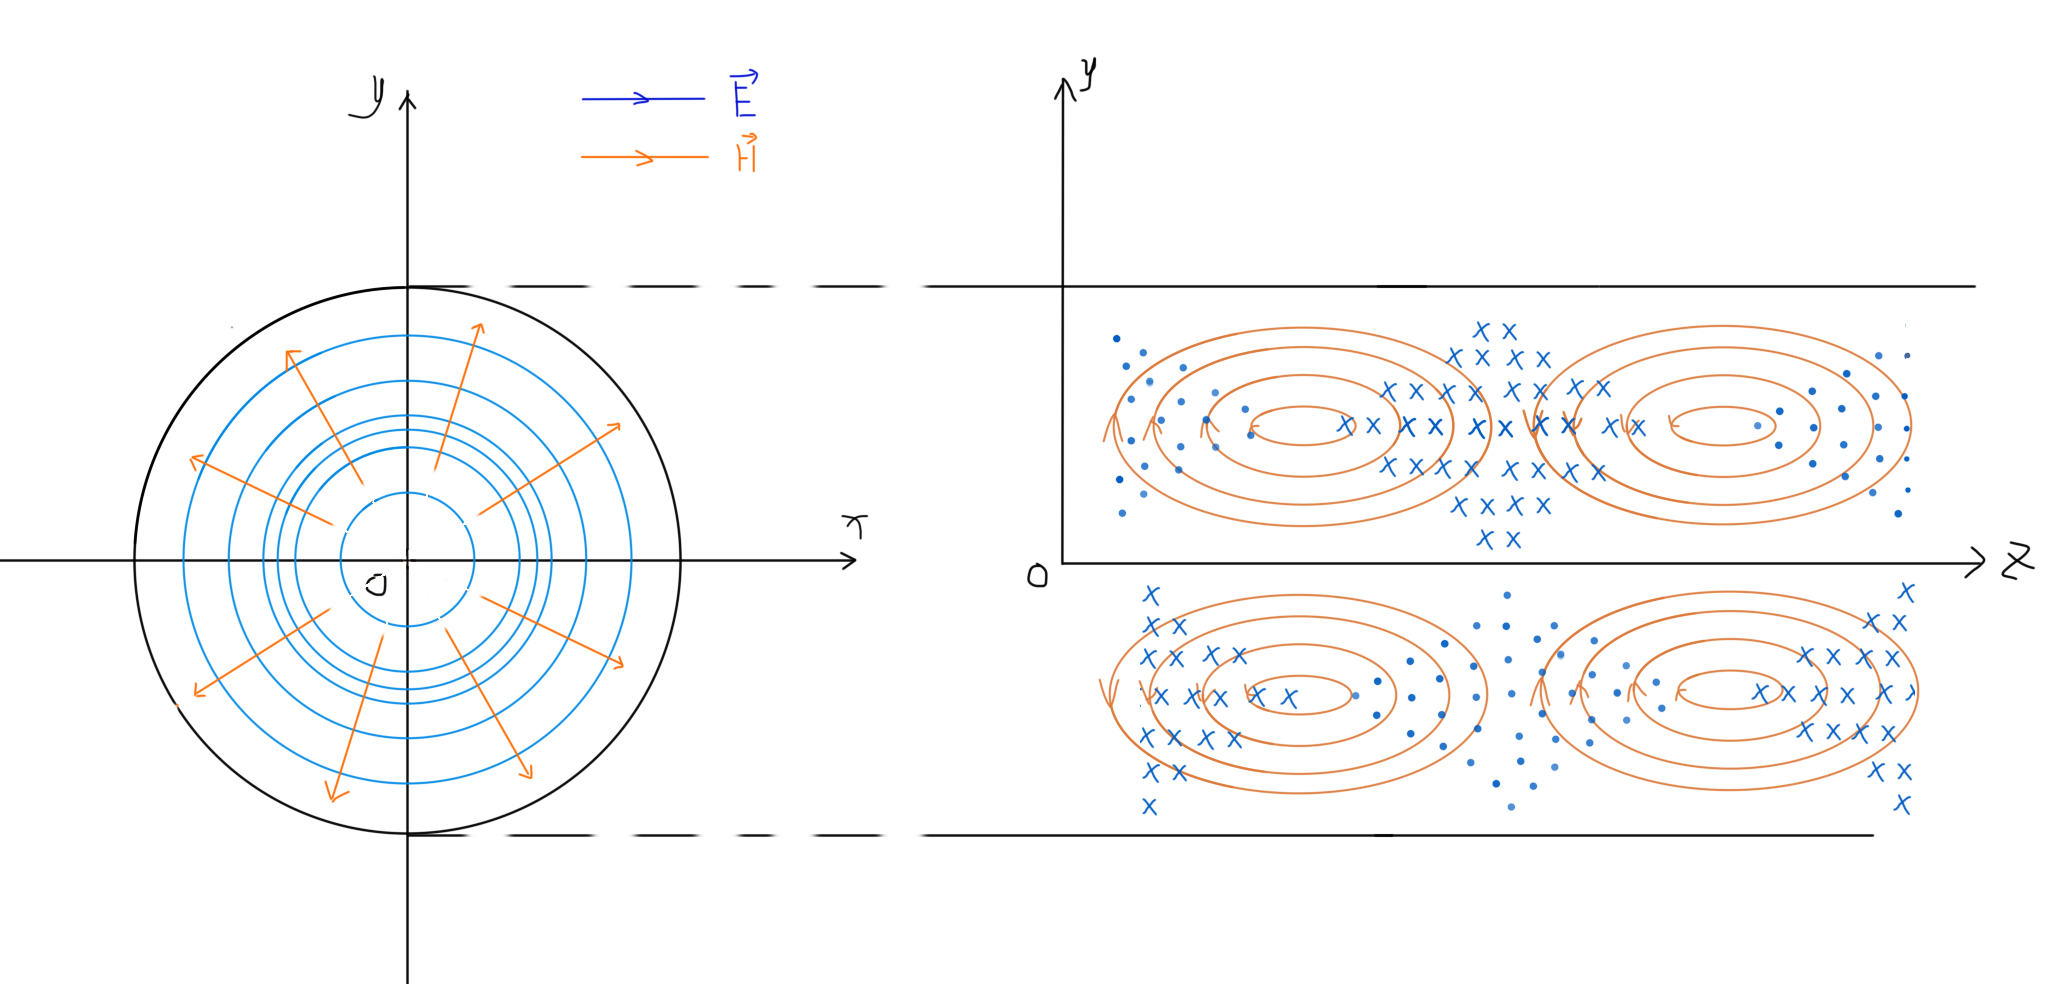
\includegraphics[width=15cm]{figure/appendix/2-6(3).jpg}
        \caption{\kaishu 2-6第三题图}\label{Fig: 2-6(3)}
    \end{figure}
    \\[15pt]
    \paragraph{4}已知半径为R的圆波导,磁场有唯一分量
    \begin{equation*}
        H_\phi=H_0 \mathrm{J}_0'\left(\frac{\nu_{01}}{R}r\right)\mathrm{e}^{-\mathrm{j}\beta z}
    \end{equation*}
    \begin{enumerate}
        \renewcommand*\labelenumi{(\theenumi)} %设置enumerate标号为一对圆括号
        \item 它是TE还是TM模式?
        \item 求磁场$\vec{E}$;
        \item 分析它的模式指数$m,n$并说出其物理意义;
        \item 画出场型图。
    \end{enumerate}
    ~\\{\bfseries 解:}\\
    (1):由于磁场没有纵向分量,因此为TM模式。\\
    (2):根据递推公式
    \begin{equation*}
        x \mathrm{J}_m'\left(x\right)+m \mathrm{J}_m\left(x\right)=x \mathrm{J}_{m-1}\left(x\right)
    \end{equation*}
    有
    \begin{equation*}
        \mathrm{J}_0'\left(x\right)=-\mathrm{J}_1\left(x\right)
    \end{equation*}
    因此,
    $\vec{E}=\frac{1}{\mathrm{j}\omega\varepsilon}\nabla\times\vec{H}$,在柱坐标系下:
    \begin{align}
        \vec{E}&=\frac{1}{\mathrm{j}\omega\varepsilon}\cdot\frac{1}{r}\begin{vmatrix}
            \hat{r}&r\hat{\phi}&\hat{z}\\
            \frac{\partial }{\partial r}&\frac{\partial }{\partial \phi}&\frac{\partial }{\partial z}\\
            H_r&rH_\phi&H_z
        \end{vmatrix}\\
        &=\frac{1}{\mathrm{j}\omega\varepsilon}\cdot\frac{1}{r}\begin{vmatrix}
            \hat{r}&r\hat{\phi}&\hat{z}\\
            \frac{\partial }{\partial r}&\frac{\partial }{\partial \phi}&\frac{\partial }{\partial z}\\
            0&rH_0 \mathrm{J}_0'\left(\frac{\nu_{01}}{R}r\right)\mathrm{e}^{-\mathrm{j}\beta z}&0
        \end{vmatrix}\notag\\
        &=\frac{1}{\mathrm{j}\omega\varepsilon r}\left[\hat{r}\mathrm{j}\beta rH_0 \mathrm{J}_0'\left(\frac{\nu_{01}}{R}r\right)\mathrm{e}^{-\mathrm{j}\beta z}+\hat{z}H_0 \mathrm{e}^{-\mathrm{j}\beta z}\frac{\partial r\mathrm{J}_0'\left(\frac{\nu_{01}}{R}r\right)}{\partial r}\right]\notag\\
        &=\frac{\mathrm{j}}{\omega\varepsilon r}\left[\hat{r}\mathrm{j}\beta rH_0 \mathrm{J}_1\left(\frac{\nu_{01}}{R}r\right)\mathrm{e}^{-\mathrm{j}\beta z}+\hat{z}H_0 \mathrm{e}^{-\mathrm{j}\beta z}\frac{\partial r\mathrm{J}_1\left(\frac{\nu_{01}}{R}r\right)}{\partial r}\right]\notag
    \end{align}

    代入$\frac{\partial r\mathrm{J}_1\left(\frac{\nu_{01}}{R}r\right)}{\partial r}=\frac{\partial\left[(\frac{\nu_{01}}{R}r)\mathrm{J}_1\left(\frac{\nu_{01}}{R}r\right)\right]}{\partial (\frac{\nu_{01}}{R}r)}=\frac{\nu_{01}}{R}r \mathrm{J}_0\left(\frac{\nu_{01}}{R}r\right)$,
    \begin{equation*}
        \vec{E}=\frac{H_0}{\omega\varepsilon}\mathrm{e}^{-\mathrm{j}\beta z}\left[-\hat{r}\beta \mathrm{J}_1\left(\frac{\nu_{01}}{R}r \right)+\hat{z}\frac{\nu_{01}}{R}\mathrm{J}_0\left(\frac{\nu_{01}}{R}r \right)\right]
    \end{equation*}
    (3): TM{\scriptsize 01}模。\\
    $m=0$,表示$\phi$方向上没有驻波,即$H_\phi,E_r$不随$\phi$改变。\\$n=1$,表示$r$方向上$E_\phi,H_r$有一个最大值。
    \begin{figure}[htp]
        \centering
        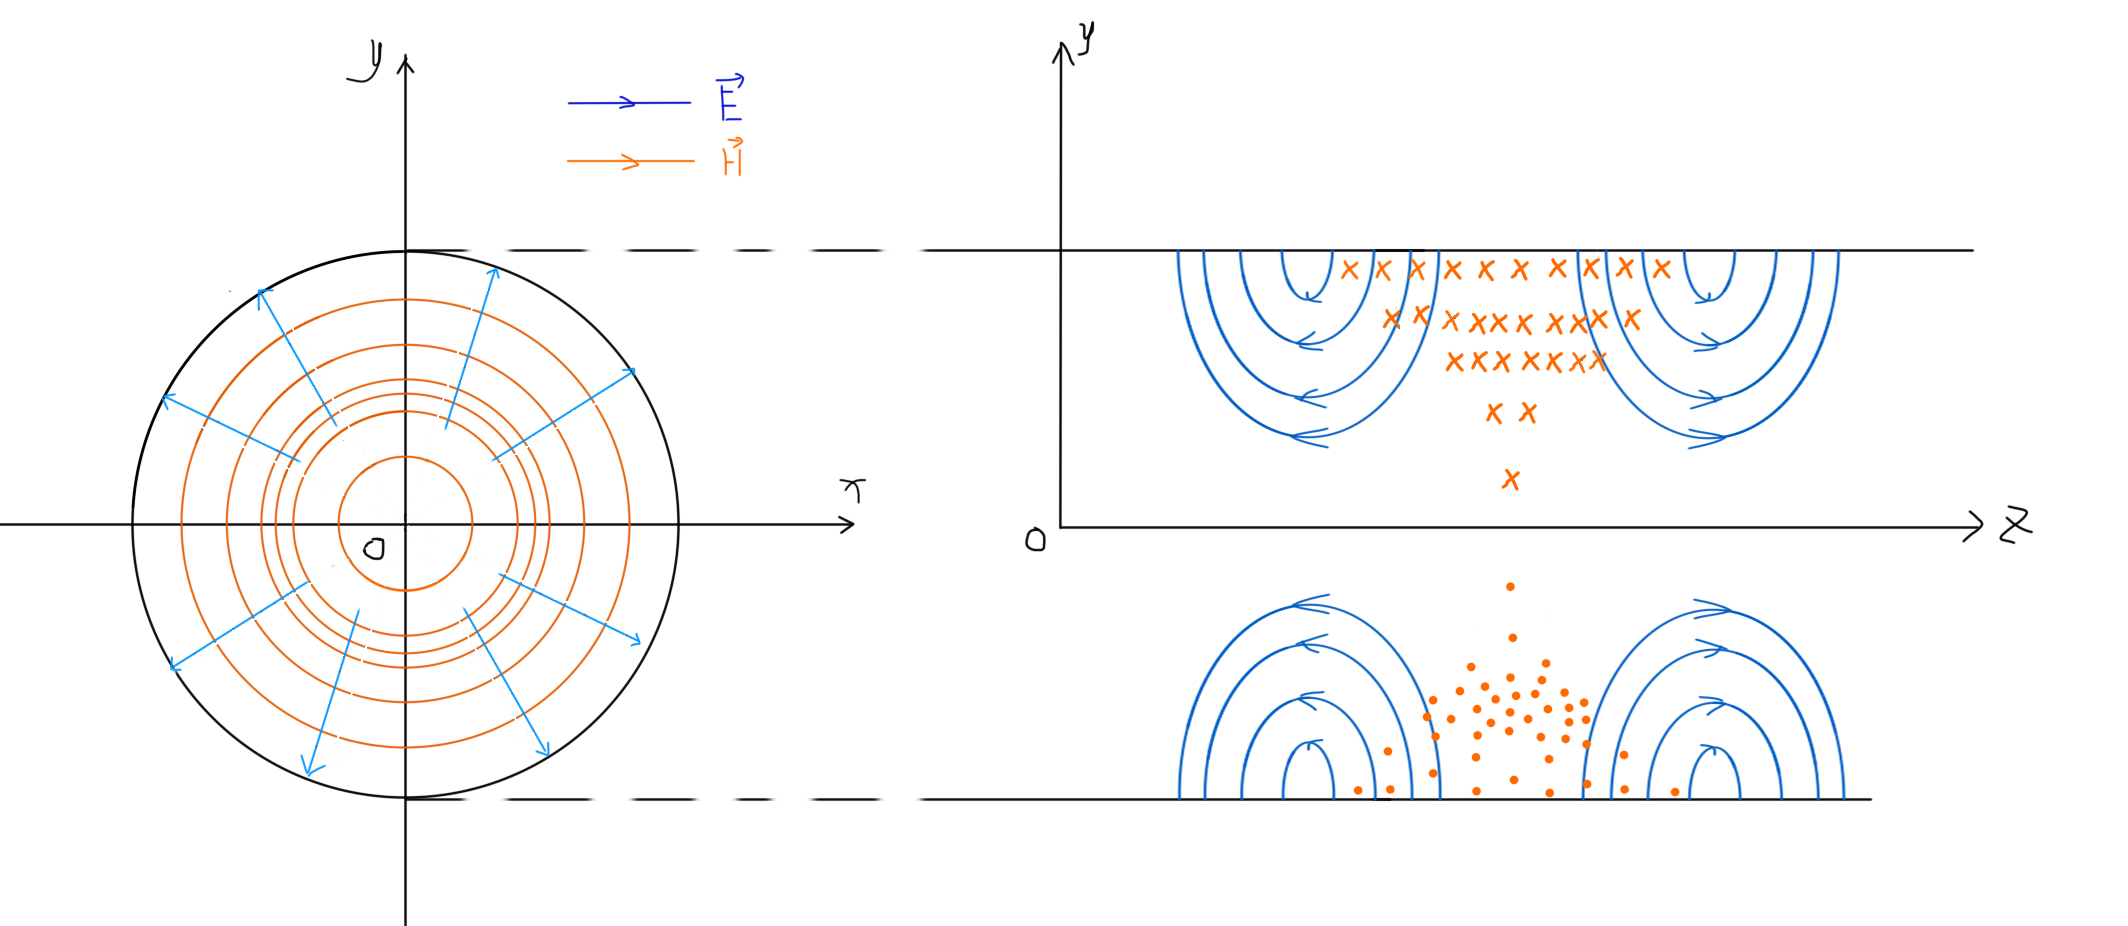
\includegraphics[width=15cm]{figure/appendix/2-6(4).jpg}
        \caption{\kaishu 2-6第四题图}\label{Fig: 2-6(4)}
    \end{figure}
    \\[15pt]
    \newpage
    \paragraph{5}横截面为半圆形波导,半径R。解出其中的 TE模和TM模。
    \\{\bfseries 解:}\\
    柱坐标下的亥姆霍兹方程:
    \begin{subequations}
        \begin{numcases}{}
            \nabla^2E_z+k^2E_z=0 \\
            \nabla^2H_z+k^2H_z=0
        \end{numcases}
    \end{subequations}
    其中
    \begin{equation}
        \nabla^2=\frac{1}{r}\frac{\partial }{\partial r}\left(r \frac{\partial }{\partial r}\right)+\frac{1}{r^2}\frac{\partial^2}{\partial \phi^2}+\frac{\partial^2}{\partial z^2}
    \end{equation}
    \begin{enumerate}
        \renewcommand*\labelenumi{\circled{\theenumi}}
        \item TE模:设
        \begin{equation}
            H_z=R(r)\varPhi(\phi)\mathrm{e}^{-\gamma z}\label{Equ: variables speration of Hz}
        \end{equation}
        展开亥姆霍兹方程,得
        \begin{equation}
            \frac{\partial^2H_z}{\partial r^2}+\frac{1}{r}\frac{\partial H_z}{\partial r}+\frac{1}{r^2}\frac{\partial^2H_z}{\partial \phi^2}+(\gamma^2+k^2)H_z=0\label{Equ: Helmholtz equation of Hz in cylindrical coordinate}
        \end{equation}
        令$\gamma^2+k^2=k_c^2$,并假设常数$m^2$,满足
        \begin{equation}
            \frac{1}{\varPhi}\frac{\mathrm{d}^2\varPhi}{\mathrm{d}\phi^2}=-m^2\label{Equ-Def: -m^2}
        \end{equation}
        代入式(\ref{Equ: variables speration of Hz})和式(\ref{Equ-Def: -m^2}),将方程(\ref{Equ: Helmholtz equation of Hz in cylindrical coordinate})整理为:
        \begin{equation}
            r^2 \frac{\mathrm{d}^2R}{\mathrm{d}r^2}+r \frac{\mathrm{d}R}{\mathrm{d}r}+(k_c^2r^2-m^2)R=0
        \end{equation}
        其通解为:
        \begin{subequations}
            \begin{numcases}{}
                \Phi(\phi)=c_1\cos m\phi+c_2\sin m\phi=\begin{pmatrix}
                    \cos m\phi\\\sin m\phi
                \end{pmatrix}\\
                R(r)=c_3 \mathrm{J}_m\left(k_cr\right)+c_4 \mathrm{N}_m\left(k_cr\right)=\begin{pmatrix}
                    \mathrm{J}_m\left(k_cr\right)\\\mathrm{N}_m\left(k_cr\right)
                \end{pmatrix}
            \end{numcases}
        \end{subequations}
        根据圆波导的特点和 Neumann 函数的性质,$R(r)$只应含有$c_3\mathrm{J}_m\left(k_cr\right)$项。因此:
        \begin{equation}
            H_z=H_0 \mathrm{J}_m\left(k_cr\right)\begin{pmatrix}
                    \cos m\phi\\\sin m\phi
                \end{pmatrix}\mathrm{e}^{-\gamma z}
        \end{equation}
        由纵向分量法,
        \begin{equation}
            \begin{bmatrix}
                E_r\\E_\phi\\H_r\\H_\phi
            \end{bmatrix}
            =\frac{1}{k_c^2}\begin{bmatrix}
                -\gamma&0&0&-\mathrm{j}\omega \mu\\
                0&-\gamma&\mathrm{j}\omega \mu&0\\
                0&\mathrm{j}\omega \varepsilon&-\gamma&0\\
                -\mathrm{j}\omega \varepsilon&0&0&-\gamma\\
            \end{bmatrix}
            \begin{bmatrix}
                \frac{\partial E_z}{\partial r}\\\frac{1}{r}\frac{\partial E_z}{\partial \phi}\\\frac{\partial H_z}{\partial r}\\\frac{1}{r}\frac{\partial H_z}{\partial \phi}
            \end{bmatrix}
        \end{equation}
        得(半)圆柱形波导TE模场的一般解:
        \begin{subequations}
            \begin{numcases}{}
                E_z=0 \\
                H_z=H_0 \mathrm{J}_m\left(k_cr\right)\begin{pmatrix}
                    \cos m\phi\\\sin m\phi
                \end{pmatrix}\mathrm{e}^{-\gamma z} \\
                E_r=\pm H_0\frac{\mathrm{j}\omega\mu m}{k_c^2r}\mathrm{J}_m\left(k_cr\right)\begin{pmatrix}
                    \sin m\phi\\\cos m\phi
                \end{pmatrix}\mathrm{e}^{-\gamma z} \\
                E_\phi=H_0\frac{\mathrm{j}\omega\mu}{k_c}\mathrm{J}_m'\left(k_cr\right)\begin{pmatrix}
                    \cos m\phi\\\sin m\phi
                \end{pmatrix}\mathrm{e}^{-\gamma z} \\
                H_r=-H_0\frac{\gamma}{k_c}\mathrm{J}_m'\left(k_cr\right)\begin{pmatrix}
                    \cos m\phi\\\sin m\phi
                \end{pmatrix}\mathrm{e}^{-\gamma z} \\
                H_\phi=\pm H_0\frac{\gamma m}{k_c^2r}\mathrm{J}_m\left(k_cr\right)\begin{pmatrix}
                    \sin m\phi\\\cos m\phi
                \end{pmatrix}\mathrm{e}^{-\gamma z}
            \end{numcases}\label{Equs: General Solution of TE Field in Half-cylinder}
        \end{subequations}\\
        由波导在$\phi$方向上的周期边界条件,可知$m\in\mathbb{Z}$;\\
        由半圆柱形波导的理想导体边界条件:
        \begin{subequations}
            \begin{numcases}{}
                E_r(\phi=0)=E_r(\phi=\pi)=0 \\
                E_\phi(r=R,0<\phi<\pi)=0
            \end{numcases}
        \end{subequations}
        代入式(\ref{Equs: General Solution of TE Field in Half-cylinder})中,得:
        \begin{subequations}
            \begin{numcases}{}
                H_0\frac{\mathrm{j}\omega\mu m}{k_c^2r}\mathrm{J}_m\left(k_cr\right)\begin{pmatrix}
                    0\\1
                \end{pmatrix}\mathrm{e}^{-\gamma z}=
                H_0\frac{\mathrm{j}\omega\mu m}{k_c^2r}\mathrm{J}_m\left(k_cr\right)\begin{pmatrix}
                    0\\\cos{m\pi}
                \end{pmatrix}\mathrm{e}^{-\gamma z}=0\label{Equ: TE boundary conditions NO.1 in Half-cylinder}\\
                H_0\frac{\mathrm{j}\omega\mu}{k_c}\mathrm{J}_m'\left(k_cR\right)\begin{pmatrix}
                    \cos m\phi\\\sin m\phi
                \end{pmatrix}\mathrm{e}^{-\gamma z}=0\label{Equ: TE boundary conditions NO.2 in Half-cylinder}
            \end{numcases}
        \end{subequations}
        由式(\ref{Equ: TE boundary conditions NO.2 in Half-cylinder}),可推知$\mathrm{J}_m'\left(k_cR\right)=0$,解得:
        \begin{equation}
            k_c=\frac{\mu_{mn}}{R}\,,\;n=1,2,\cdots
        \end{equation}
        其中$\mu_{mn}$为第一类$m$阶Bessel函数\underline{\bfseries 导数}的第$n$个根。\\
        式(\ref{Equ: TE boundary conditions NO.1 in Half-cylinder})中,由于$\mathrm{J}_m\left(k_cr\right)$仍可以取特定范围内的任意值,可推知待定系数$c_2=0$。\\
        因此,半圆柱形波导TE模场的解为
        \begin{subequations}
            \begin{numcases}{}
                E_z=0 \\
                H_z=H_0 \mathrm{J}_m\left(\frac{\mu_{mn}}{R}r\right)\cos (m\phi)\mathrm{e}^{-\gamma z} \\
                E_r=\pm H_0\frac{\mathrm{j}\omega\mu m}{k_c^2r}\mathrm{J}_m\left(\frac{\mu_{mn}}{R}r\right) \sin (m\phi)\mathrm{e}^{-\gamma z} \\
                E_\phi=H_0\frac{\mathrm{j}\omega\mu}{k_c}\mathrm{J}_m'\left(\frac{\mu_{mn}}{R}r\right)\cos (m\phi)\mathrm{e}^{-\gamma z} \\
                H_r=-H_0\frac{\gamma}{k_c}\mathrm{J}_m'\left(\frac{\mu_{mn}}{R}r\right)\cos (m\phi)\mathrm{e}^{-\gamma z} \\
                H_\phi=\pm H_0\frac{\gamma m}{k_c^2r}\mathrm{J}_m\left(\frac{\mu_{mn}}{R}r\right)\sin (m\phi)\mathrm{e}^{-\gamma z}
            \end{numcases}
        \end{subequations}
        ~\\[8pt]
        \item TM模:\\同理利用纵向场分量法,可以导出(半)圆柱形波导TM模场的一般解:
        \begin{subequations}
            \begin{numcases}{}
                E_z=E_0 \mathrm{J}_m\left(k_cr\right)\begin{pmatrix}
                    \cos m\phi\\\sin m\phi
                \end{pmatrix}\mathrm{e}^{-\gamma z} \\
                H_z=0\\
                E_r=-E_0\frac{\gamma}{k_c}\mathrm{J}_m'\left(k_cr\right)\begin{pmatrix}
                    \cos m\phi\\\sin m\phi
                \end{pmatrix}\mathrm{e}^{-\gamma z} \\
                E_\phi=\pm E_0\frac{\gamma m}{k_c^2r}\mathrm{J}_m\left(k_cr\right)\begin{pmatrix}
                    \sin m\phi\\\cos m\phi
                \end{pmatrix}\mathrm{e}^{-\gamma z} \\
                H_r=\mp E_0\frac{\mathrm{j}\omega\varepsilon m}{k_c^2r}\mathrm{J}_m\left(k_cr\right)\begin{pmatrix}
                    \sin m\phi\\\cos m\phi
                \end{pmatrix}\mathrm{e}^{-\gamma z} \\
                H_\phi=-E_0\frac{\mathrm{j}\omega\varepsilon}{k_c}\mathrm{J}_m'\left(k_cr\right)\begin{pmatrix}
                    \cos m\phi\\\sin m\phi
                \end{pmatrix}\mathrm{e}^{-\gamma z}
            \end{numcases}\label{Equs: General Solution of TM Field in Half-cylinder}
        \end{subequations}\\
        由波导在$\phi$方向上的周期边界条件,可知$m\in\mathbb{Z}$;\\
        由半圆柱形波导的理想导体边界条件:
        \begin{subequations}
            \begin{numcases}{}
                E_r(\phi=0)=E_r(\phi=\pi)=0 \\
                E_\phi(r=R,0<\phi<\pi)=0
            \end{numcases}
        \end{subequations}
        代入式(\ref{Equs: General Solution of TE Field in Half-cylinder})中,得:
        \begin{subequations}
            \begin{numcases}{}
                E_0\frac{\gamma}{k_c}\mathrm{J}_m'\left(k_cr\right)\begin{pmatrix}
                    1\\0
                \end{pmatrix}\mathrm{e}^{-\gamma z}=
                E_0\frac{\gamma}{k_c}\mathrm{J}_m'\left(k_cr\right)\begin{pmatrix}
                    \cos m\pi\\0
                \end{pmatrix}\mathrm{e}^{-\gamma z}=0\label{Equ: TM boundary conditions NO.1 in Half-cylinder}\\
                E_0\frac{\gamma m}{k_c^2R}\mathrm{J}_m\left(k_cR\right)\begin{pmatrix}
                    \sin m\phi\\\cos m\phi
                \end{pmatrix}\mathrm{e}^{-\gamma z}=0\label{Equ: TM boundary conditions NO.2 in Half-cylinder}
            \end{numcases}
        \end{subequations}
        由式(\ref{Equ: TE boundary conditions NO.2 in Half-cylinder}),可推知$\mathrm{J}_m\left(k_cR\right)=0$,解得:
        \begin{equation}
            k_c=\frac{\nu_{mn}}{R}\,,\;n=1,2,\cdots
        \end{equation}
        其中$\nu_{mn}$为第一类$m$阶Bessel函数的第$n$个根。\\
        式(\ref{Equ: TE boundary conditions NO.1 in Half-cylinder})中,由于$\mathrm{J}_m'\left(k_cr\right)$仍可以取特定范围内的任意值,可推知待定系数$c_1=0$。\\
        因此,半圆柱形波导TE模场的解为
        \begin{subequations}
            \begin{numcases}{}
                E_z=E_0 \mathrm{J}_m\left(\frac{\nu_{mn}}{R}r\right)\sin (m\phi) \mathrm{e}^{-\gamma z} \\
                H_z=0\\
                E_r=-E_0\frac{\gamma}{k_c}\mathrm{J}_m'\left(\frac{\nu_{mn}}{R}r\right)\sin (m\phi) \mathrm{e}^{-\gamma z} \\
                E_\phi=\pm E_0\frac{\gamma m}{k_c^2r}\mathrm{J}_m\left(\frac{\nu_{mn}}{R}r\right)\cos (m\phi)\mathrm{e}^{-\gamma z} \\
                H_r=\mp E_0\frac{\mathrm{j}\omega\varepsilon m}{k_c^2r}\mathrm{J}_m\left(\frac{\nu_{mn}}{R}r\right)\cos (m\phi)\mathrm{e}^{-\gamma z} \\
                H_\phi=-E_0\frac{\mathrm{j}\omega\varepsilon}{k_c}\mathrm{J}_m'\left(\frac{\nu_{mn}}{R}r\right)\sin (m\phi) \mathrm{e}^{-\gamma z}
            \end{numcases}
        \end{subequations}
    \end{enumerate}

    \section{作业2-7}
    \begin{center}
        姓名:韩玉千\hspace{4cm}学号:19020100423
    \end{center}

    \paragraph{1}论述TEM模传输线的主要特点,并说明它们满足什么支配方程。
    \\{\bfseries 解:}\\
        TEM传输线上,电场和磁场没有纵向分量:
        \begin{subequations}
            \begin{numcases}{\mbox{TEM模:}}
                \vec{E}_z=0 \\
                \vec{H}_z=0
            \end{numcases}
        \end{subequations}

    TEM模所满足的支配方程:\emph{Maxwell}方程组。

    \paragraph{2}导出圆同轴线的功率$P$和导体衰减常数$\alpha_c$的表达式。
    \\{\bfseries 解:}\\
    在圆同轴线中,电磁场分布:
    \begin{subequations}
        \begin{numcases}{}
            \vec{E}=\hat{r} E_0\frac{a}{r}\mathrm{e}^{-\mathrm{j}\beta z} \\
            \vec{H}=\hat{\varphi} \frac{E_0}{\eta}\frac{a}{r}\mathrm{e}^{-\mathrm{j}\beta z}
        \end{numcases}
    \end{subequations}
    同轴线内外导体间电压和内导体的轴向电流:
    \begin{subequations}
        \begin{numcases}{}
            U=\int_{a}^{b}E_r\,\mathrm{d}r=E_0a\ln\left(\frac{b}{a}\right)\mathrm{e}^{-\mathrm{j}\beta z} \\
            I=\left[\int_{0}^{2\pi}H_\varphi\,r\mathrm{d}\varphi\right]_{r=a}=\frac{2\pi E_0a}{\eta}\mathrm{e}^{-\mathrm{j}\beta z}
        \end{numcases}
    \end{subequations}
    平均坡印廷矢量:
    \begin{equation}
        \vec{S}_{av}=\Re\left[\frac{1}{2}\vec{E}\times \vec{H}^*\right]=\hat{z}\frac{E_0^2a^2}{2\eta r^2}
    \end{equation}
    因此,传输功率:
    \begin{equation}
        P=\int_{a}^{b}S_{av}\,2\pi r\mathrm{d}r=\frac{\sqrt{\varepsilon_r}}{120}E_0^2a^2\ln\left(\frac{b}{a}\right)
    \end{equation}
    衰减常数:
    \begin{equation}
        \alpha_c=\frac{8.686R_s\sqrt{\varepsilon_r}\left(1+\frac{b}{a}\right)}{2\pi b\left(120\ln\frac{b}{a}\right)}\qquad\si{\decibel\per\meter}
    \end{equation}

    \paragraph{3}研究如图所示的半填充圆同轴线。
    \begin{enumerate}
        \renewcommand*\labelenumi{(\theenumi)}
        \item 电场 $\vec{E}$和磁场 $\vec{H}$表达式。
        \item 传输波长$\lambda$。
        \item 波速$v_p$。
        \item 特性阻抗$Z_0$。
    \end{enumerate}
    \begin{figure}[htp]
        \centering
        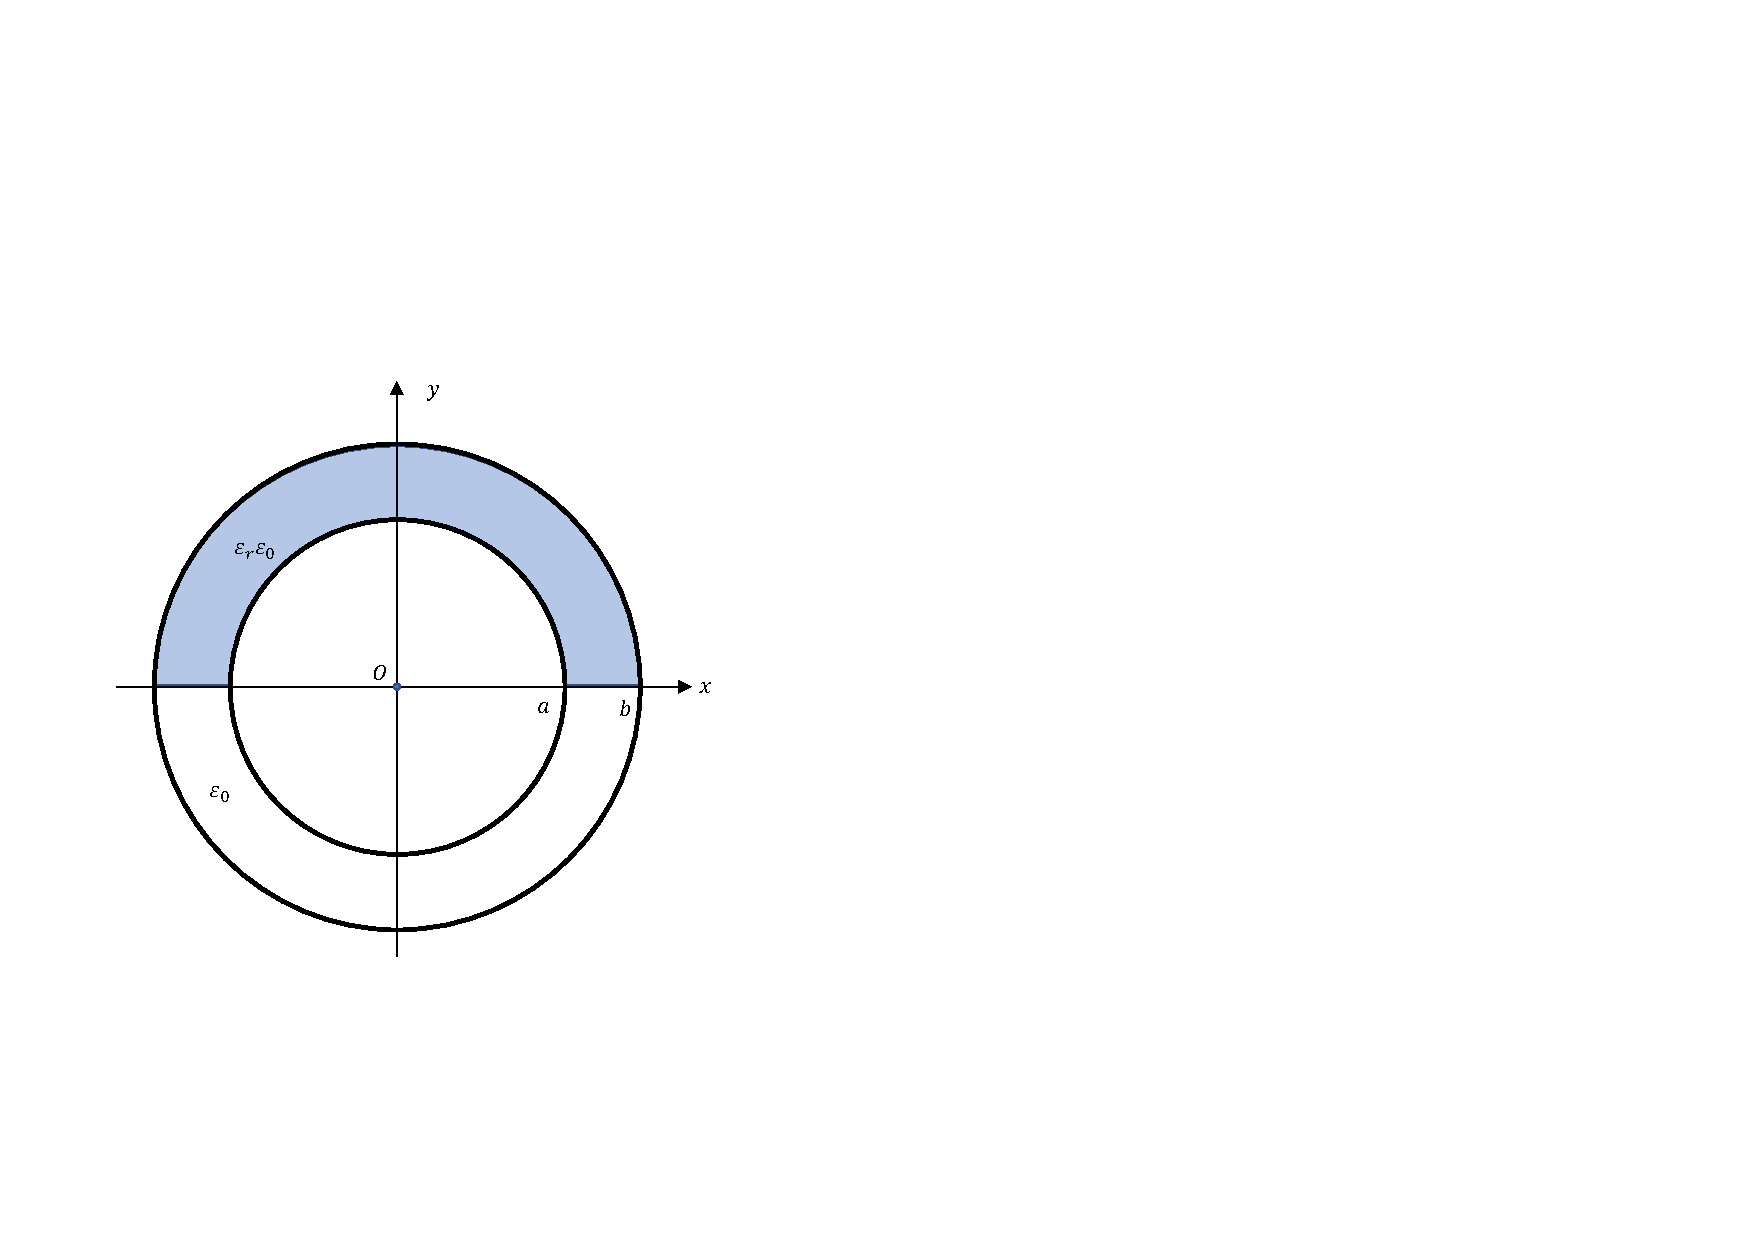
\includegraphics[width=6cm]{figure/appendix/2-7(3).pdf}
        \caption{\kaishu 2-7第三题图:半填充圆同轴线}\label{Fig: 2-7(3)}
    \end{figure}
    {\bfseries 解:}\\
    (1)



    \paragraph{4}有两种不同的圆同轴线$\dfrac{a_1}{b_1}=\dfrac{a_2}{b_2}$,$a_1>a_2$。
    \begin{figure}[htp]
        \centering
        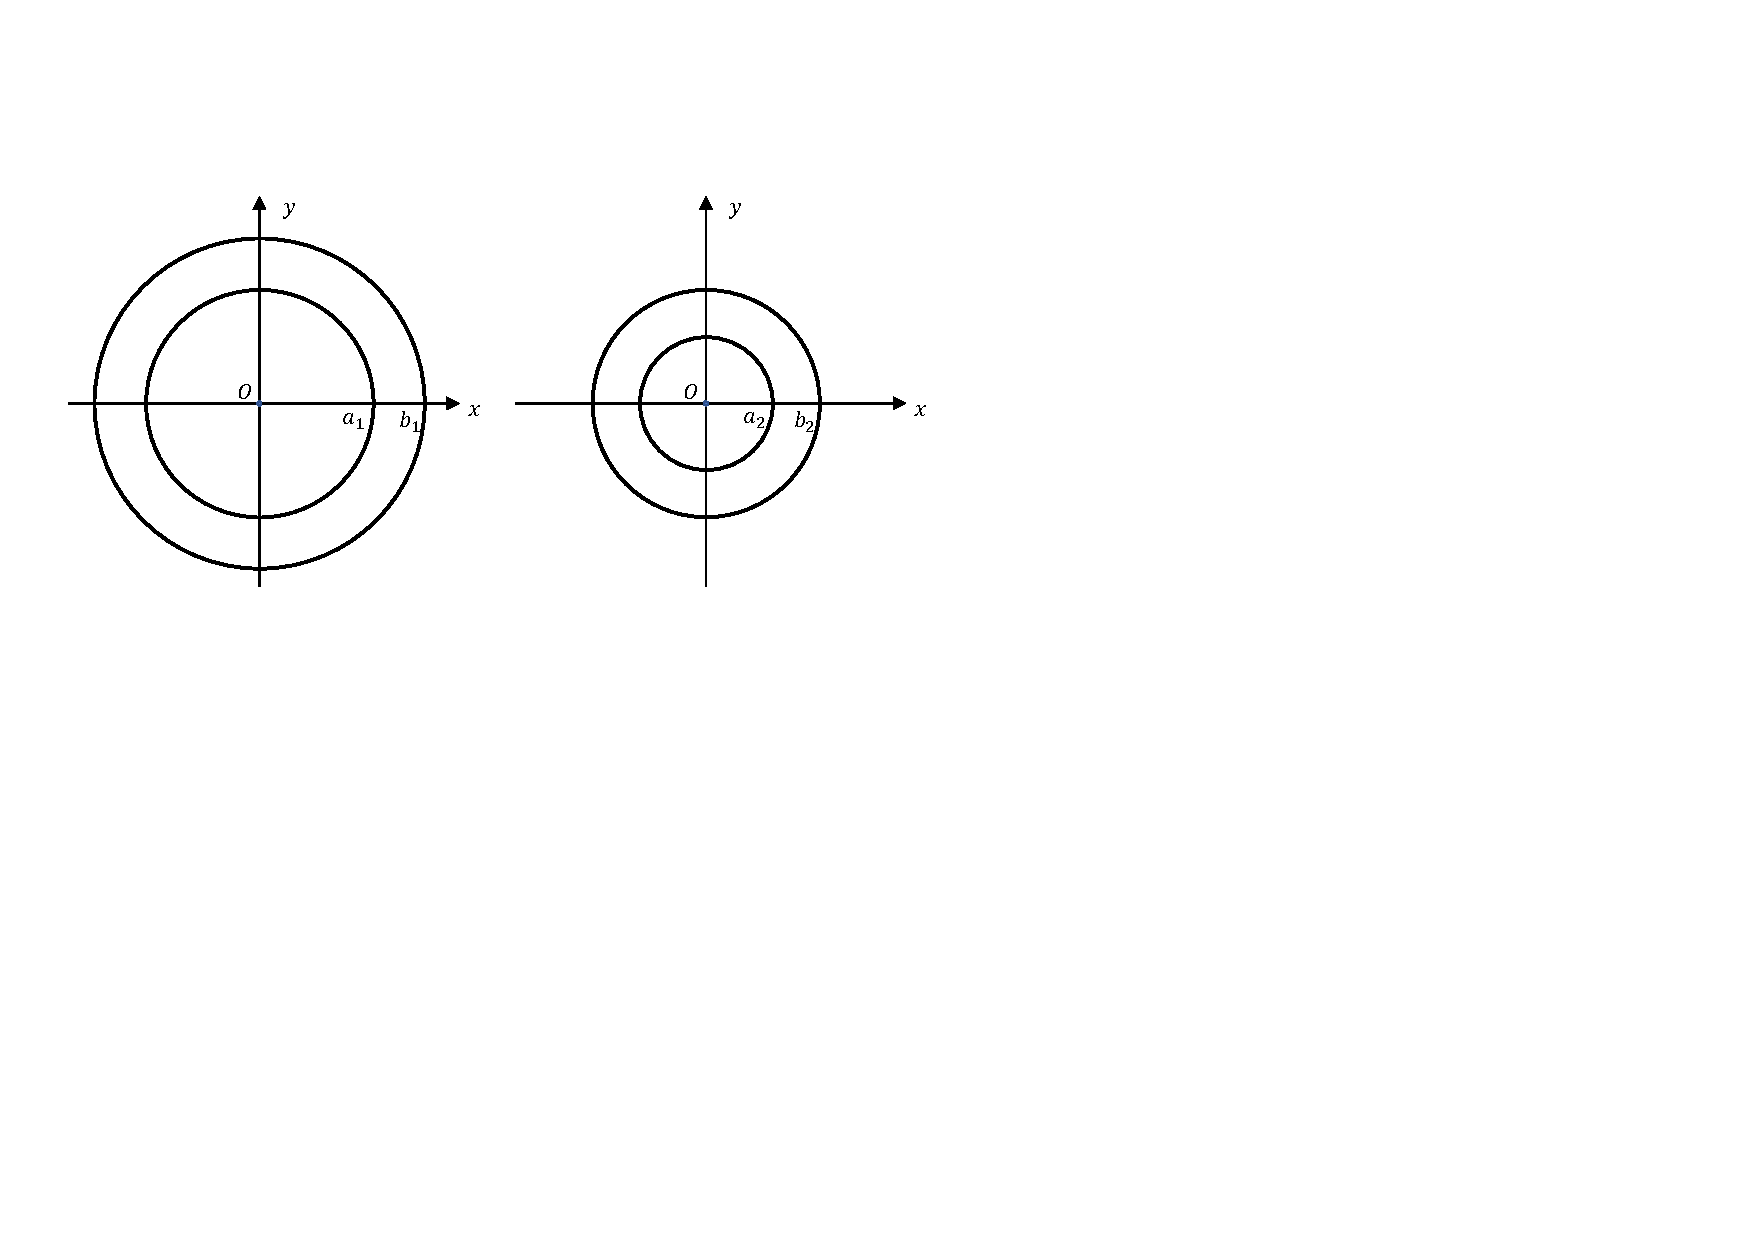
\includegraphics[width=12cm]{figure/appendix/2-7(4).pdf}
        \caption{\kaishu 2-7第四题图:两种圆同轴线}\label{Fig: 2-7(4)}
    \end{figure}
    \begin{enumerate}
        \renewcommand*\labelenumi{(\theenumi)}
        \item 哪种圆同轴线的特性阻抗$Z_0$大?
        \item 哪种圆同轴线的波长$\lambda$大?
        \item 哪种圆同轴线的功率容量$P_\mathrm{max}$大?
        \item 哪种圆同轴线的TEM模频带宽?
    \end{enumerate}
    {\bfseries 解:}\\
    (1)


    \paragraph{5}圆同轴线如下图。采用$\nabla_t^2 \vec{E}=0$和$\nabla_t^2 \vec{H}=0$求其TEM主模。已知圆对称,即$\frac{\partial }{\partial \varphi}=0$,且$\vec{E}=\hat{r}E$,$\vec{H}=\hat{\varphi}H$。

    \begin{figure}[htp]
        \centering
        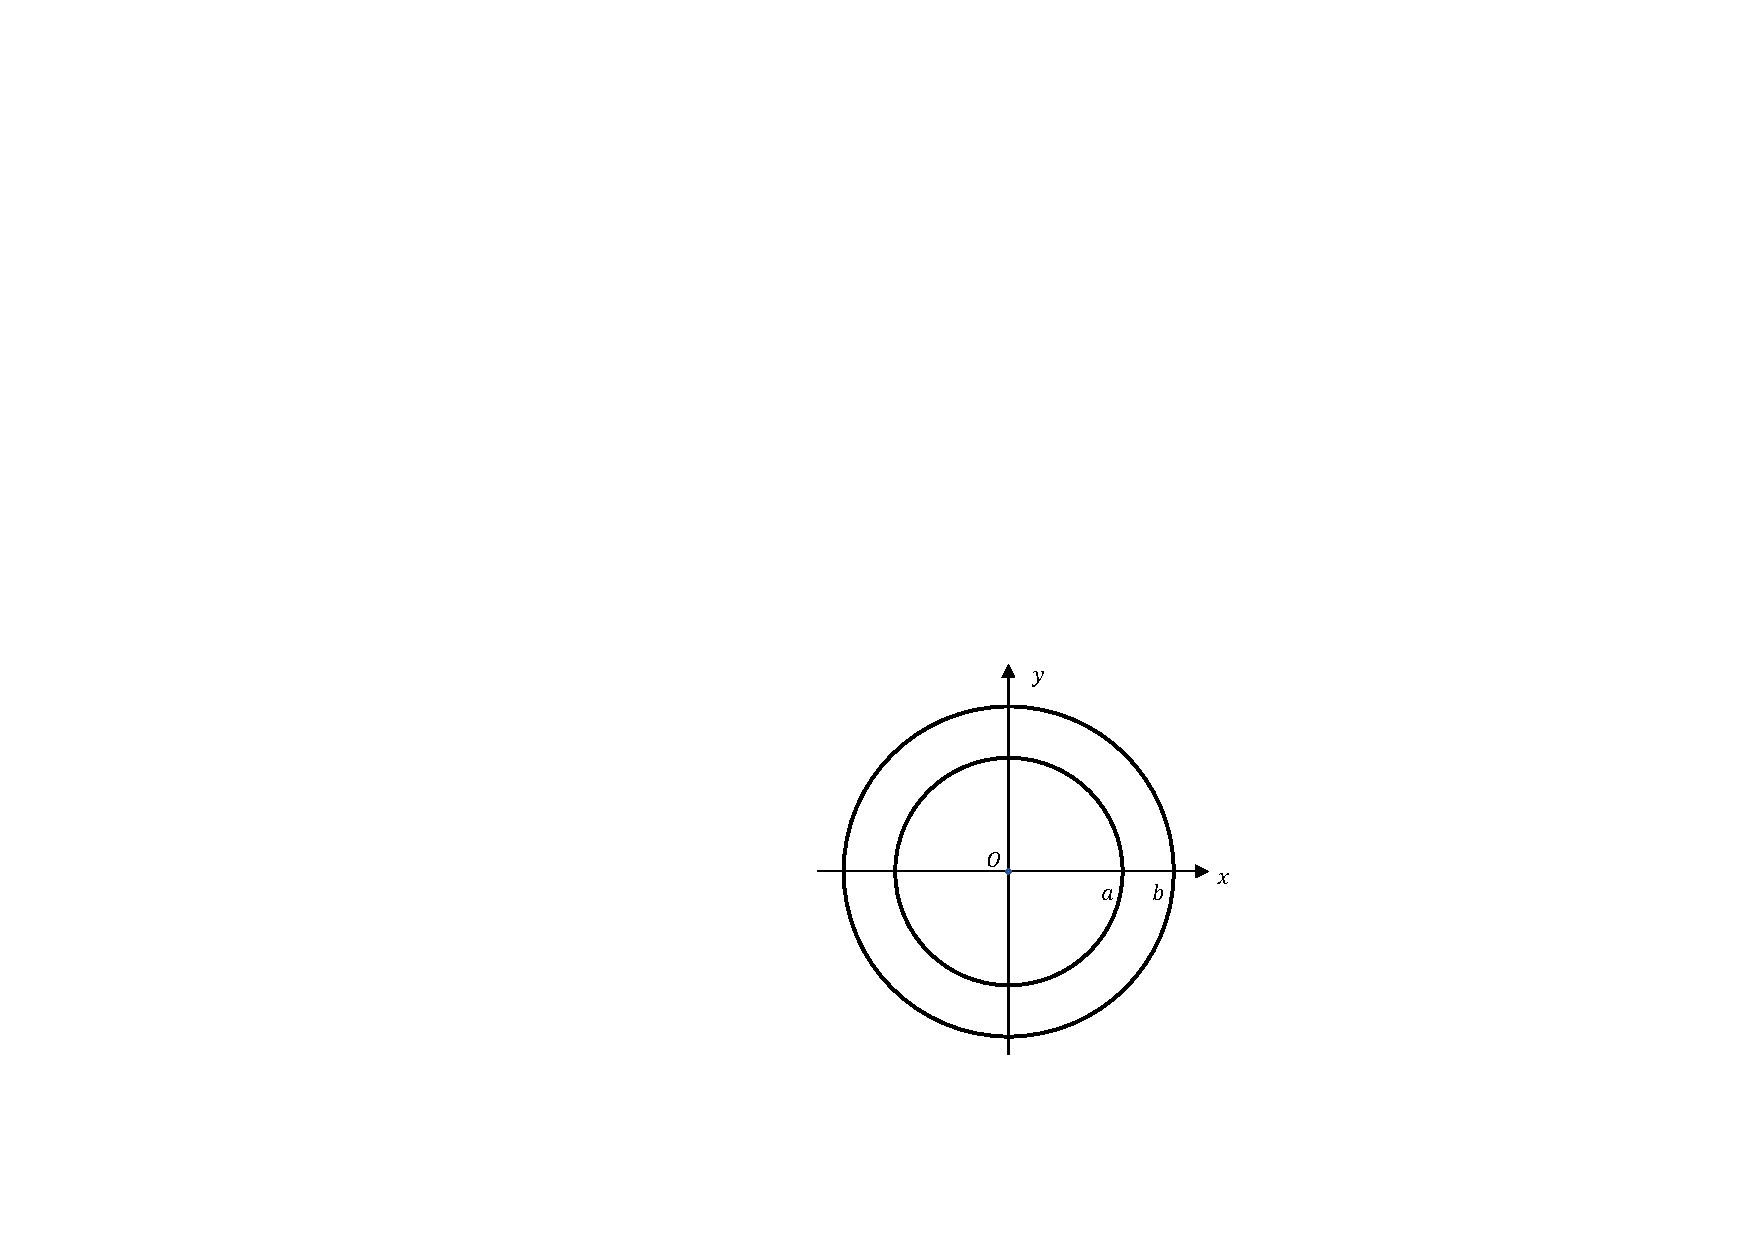
\includegraphics[width=6cm]{figure/appendix/2-7(5).pdf}
        \caption{\kaishu 2-7第五题图:圆同轴线}\label{Fig: 2-7(5)}
    \end{figure}

    {\bfseries 解:}\\

\end{appendices}

\end{document}